\documentclass[11pt]{article}
\usepackage{amsthm}
\usepackage{amsmath}
\usepackage{amssymb}
\usepackage[spanish,es-tabla]{babel}
\usepackage[style=numeric,sorting=none]{biblatex}
\usepackage{bm}
\usepackage{booktabs}
\usepackage{enumitem}a
\usepackage{fancyhdr}
\usepackage{float}
\usepackage[utf8]{inputenc}
\usepackage{listingsutf8}
\usepackage[top=2.5cm,bottom=2.5cm,left=2.5cm,right=2.5cm]{geometry}
\usepackage{graphicx}
\usepackage{longtable}
\usepackage{subcaption}
\usepackage{verbatim}
\usepackage{xcolor}

\definecolor{codegreen}{rgb}{0,0.6,0}
\definecolor{codegray}{rgb}{0.5,0.5,0.5}
\definecolor{codepurple}{rgb}{0.58,0,0.82}
\definecolor{backcolour}{rgb}{0.99,0.995,0.99}

\lstdefinestyle{mystyle}{
    backgroundcolor=\color{backcolour},   
    commentstyle=\color{codegreen},
    keywordstyle=\color{magenta},
    numberstyle=\tiny\color{codegray},
    stringstyle=\color{codepurple},
    basicstyle=\ttfamily\small,
    breakatwhitespace=false,         
    breaklines=true,                 
    captionpos=b,                    
    keepspaces=true,                 
    numbers=left,                    
    numbersep=5pt,                  
    showspaces=false,                
    showstringspaces=false,
    showtabs=false,                  
    tabsize=2
}

\lstset{style=mystyle}
\decimalpoint
% adding references
\addbibresource{../../referencias.bib}
%auxiliar commands
\newcommand{\work}{Tarea-Examen 3: Aprendizaje Supervisado}
%changes space between lines of equations
\setlength{\jot}{10pt}
%changes space between text and equations
\setlength{\abovedisplayskip}{100pt}
\setlength{\belowdisplayskip}{100pt}
\setlength{\abovedisplayshortskip}{100pt}
\setlength{\belowdisplayshortskip}{100pt}
% theorem environment in case I need it
\newtheorem{theorem}{Teorema}
%make header
\pagestyle{fancy}
\fancyhf{}
\vspace{1cm}
\rhead{}
\lhead{\work}
\cfoot{\thepage}
% Text info
\title{\textbf{\work}}
\author{Curso Avanzado de Estadística. Profa. Guillermina Eslava Gómez.\\ \\ Aldo Sayeg Pasos Trejo. César Cossio Guerrero. \\ \\ Posgrado en Ciencias Matemáticas. Universidad Nacional Autónoma de México. }
\date{\today}
\begin{document}
\maketitle
\section{Problema 1}
Buscamos realizar un estudio de clasificación sobre la base de datos \texttt{Pima}, que consiste en 532 observaciones de 7 variables usadas para describir el estado de salud de las mujeres de la tribu Pima, cuya tasa de enfermedad de Diabetes Mellitus es inusualmente alda. La descripción \cite{3-1} de las variables se muestra en la tabla \ref{1-desc}.
\begin{table}[H]
    \centering
    \begin{tabular}{c|p{8cm}}
        Variable & Descripción \\
        \hline
        ``npreg'' & número de embarazos \\
        & \\
        ``glu'' & Concentración de glucosa en el plasma para una prueba oral \\
        & \\
        ``bp'' &  Presión arterial diastólica (mmHg)\\
        & \\
        ``skin'' & grueso de la piel del triceps (mm) \\
        & \\
        ``bmi'' & Índice de masa corporal (kg/$m^2$) \\
        & \\
        ``ped'' & Función pedigree para diabetes \\
        & \\
        ``age'' & Edad (años) \\
        & \\
        ``type'' & Indicador de diabetes (``yes'' o ``no'') \\
    \end{tabular}
    \caption{Descripción de las variables}
    \label{1-desc}
\end{table}
Antes de realizar cualquier estudio sobre el sistema, analizamos la relación entre sus variables analizando su correlación en la figura \ref{1-correlation}, su separación por clase en una gráfica a pares como en la figura \ref{1-classes}, por componentes principales como en \ref{1-pca} y sus distribuciones individuales en las figuras \ref{1-npreg-dist},\ref{1-glu-dist},\ref{1-bp-dist},\ref{1-skin-dist},\ref{1-bmi-dist},\ref{1-ped-dist} y \ref{1-age-dist}.
\\
\\De ese análisis, podemos concluir rápidamente que ``bmi'' presenta una alta correlación con ``skin''. Esto se puede entender claramente ya que el índice de masa corporal debe de tener un efecto claro sobre la piel en el tríceps. De igual manera, la correlación entre ``age'' y ``npreg'' es totalmente obvia debido a que el número de embarazos se relaciona directamente con la edad.
\\
\\En cuanto a las diferencias entre clases, nuevamente no se pueden observar muchas diferencias sustanciales y las que se muestran como la de la figura \ref{1-age-dist} se entiende nuevamente de manera intuitiva ya que la incidencia de Diabetes debe de ser poca en mujeres jóvenes. La diferencia entre la distribución de ``glu'' en la figura \ref{1-glu-dist} también se puede explicar de manera trivial al igual que la de la figura \ref{1-bmi-dist} al ser la obesidad un factor de riesgo para la diabetes.
\\
\\Esta análisis nos permite especular que las variables con mayor significancia estadística pueden ser ``bmi'',``glu'',``age'' y que podemos usar una sola variable pare representar variables altamente correlacionadas.En principio, nos interesa usar 4 modelos para clasificar
\begin{enumerate}[label = \alph*)]
    \item Análisis de discriminante lineal
    \item Naive Bayes
    \item Regresión logística
    \item Suppor Vector Machines (SVM)
\end{enumerate}
Yendo un poco más lejos, consideramos realizar un análsis incluyento también el Análisis de discriminante cuadrático y K-Neighbors. La figura \ref{1-gen-sizeDependence} muestra las tasas de clasificación global y local para esos modelos para distintos tamaños del conjunto de entrenamiento de los datos. La separación de los datos se realizó sin tomar en cuenta el mantener la proporcionalidad entre las clases. Notemos que la tasa aparente corresponde a la fracción $s=1.0$. Por limitaciones del poder de cómputo disponible, se realizaron $n=10$ iteraciones para las tasas no aparentes.
\\
\\ Podemos observar que, en cuanto a la tasa de error global aparente, el modelo K-Neighbors presenta el menor valor. 
\\
\\Sin embargo, pareciera intutivo pensar que las tasas no aparentes deben de mejorar si ahora forzamos a que la separación entre conjunto de entrenamiento y de prueba mantenga la proporcionalidad existen en las clases. La tabla \ref{1-gen-eq-tab} y la gráfica \ref{1-gen-eq-sizeDependence} muestran dichos resultados.
\\
\\En efecto, se muestra que las tasas no aparentes mejoran aunque no significativamente. Si pensamos en la capacidad predictiva del modelo y en el contexto del diagnóstico médico, es claro que la tasa de aceptación que más nos interesa son los falsos negativos pues nos interesa diagnosticar con mayor precisión. En ese sentido, los modelos entrenados manteniendo la proporcionalidad presentan tasas muy elevadas de error para fracciones pequeñas.
\\
\\Antes de proceder modelo por modelo, buscamos para cada variable numérica y positiva del modelo, cual es el valor $\lambda$ que maximiza la verosimilitud de una transformación Box-Cox para esa variable. Dichos valores, junto con sus intervalos de confianza, se pueden consultar en la tabla \ref{1-bxparam-tab}
\\
\\Habiendo realizado primero este análisis, ahora nos disponemos a presentar los 4 modelos relevantes.
\subsection{Análisis de discriminante lineal}
Para discriminante lineal, no hay muchso parámetros que podamos ajustar para posibles modelos. Nos enfocamos más bien en buscar transformaciones o interacciones entre las variables.
\\
\\Despues de mostrar que las transformaciones Box-Cox no presentan una mejoría sustancial para ninguno de los modelos, y que esta es considerada la mejor clase de transformaciones dado que las figuras \ref{1-correlation}, \ref{1-classes} no nos muestra que otra tranfromación podría mejorar la separación con una variable, nos limitamos a no realizar transformaciones sobre las variables.
\\
\\Así, solo añadimos posibles interacciones. Entre interacciones a pares, encontramos que la interacción que presentaba menor tasa global aparente de error era la interacción entre ``ped''  y  ``age''.
\\
\\Añadiendo esta interacción al modelo, despues consideramos interacciones terciarias que lo hagan óptimo. Sin embargo, todas las tasas de interacciones muestran tasas similares (mayores 1 0.20), por lo que no consideramos que representen una mejoría sobre nuestro modelo y, así, nos quedamos con este modelo en interacción a pares como el mejor clasificador.
\subsection{Naive Bayes}
Nuevamente, no existen muchos parámetros modificables en el método de Naive Bayes y, por los argumentos anteriormente mostrados, recurrimos a otra interacción binaria, la interacción entre ``ped'' e ``bp''.
\subsection{Regresión Logística}
Existen mejores estimadores para determinar los valores de la regresión logística. La tabla de los $p$-values para una regresión con todas las variables la podemos presentar en la tabla \ref{1-log-p}.
\\
\\
Despues de revisar la sigfinicancia estadística de la regresión, nos podemos quedar solamente con las variables ``glu'',``bmi'',``ped'' y ``age''. Ademas, considerando que la edad presenta una gran influencia, podemos incluir un término cuadrático para la edad ``age$^2$''. Así, este modelo es el que consideramos óptimo y representativo de este método.
\subsection{Support Vector Machines}
Por ser el método que presenta más parámetros para el clasificador, primero realizamos una corrida para kernels lineales, de funciones de base radial de grado 1,3 y 5 y polinomiales de los mismos grados. Los resultados se pueden consultar en la figura \ref{1-svm-eq-sizeDependence}. Aunque existen también los Kernels sigmoides \cite{sklearn-svc}, al probar con estos encontramos tasas de clasificación muy bajas, por lo que los excluimos del análisis.
\\
\\El kernel lineal se desempeña muy bien también al ser comparado por los otros. Tanto clasificadores de base radial como los polinomiales muestran muy buen desempeño aun para grados bajos. Sin embargo, el clasificador que consideramos como el óptimo es el que minimiza la tasa global aparante, es decir, \textbf{el de kernel polinomial y grado 5}.
\\
\\Por las limitaciones del poder computacional, resultó imposible analizar distintos valores del parámetro $\gamma$. Aunque ahora podríamos analizar interacciones, por la estructura de los parámetros del sistema, sabemos que estas ya se están contemplando al aumentar el grado del kernel. Así, dejamos este modelo como el definitivo para este clasificador y presentamos sus tasas de error de manera gráfica individual como tabular en la figura \ref{1-svm-fin-eq-sizeDependence}.
\subsection{Conclusiones}
Para resumir, en la tabla \ref{1-var} mostramos las variables utilizadas por el modelo correspondiente a cada método:
\begin{table}
    \centering
    \begin{tabular}{p{3cm}|p{5cm} | c}
        Método & Variables en el modelo & Notas extra\\
        \hline
        Análisis de Discriminante Lineal & ``npreg'', ``glu'', ``bp'', ``skin'', ``bmi'', ``ped'', ``age'', ``type'', ``ped*age'' & -\\
        & & \\
        Naive Bayes & ``npreg'', ``glu'', ``bp'', ``skin'', ``bmi'', ``ped'', ``age'', ``type'', ``ped*bp'' & -\\
        & & \\
        Regresión logística & ```glu'', ``bmi'', ``ped'',  ``age'',  ``age$^2$'' & - \\
        & & \\
        Support Vector Machines & ``npreg'', ``glu'', ``bp'', ``skin'', ``bmi'', ``ped'', ``age'', ``type'' & Kernel Polynomial de grado 5 \\
    \end{tabular}
    \caption{Variables de los modelos}
    \label{1-var}
\end{table}
Comparamos los cuatro modelos seleccionados para cada método. La tabla \ref{1-final-tab} y  la figura \ref{1-final-sizeDependence} muestran dicha comparación. De Inmediatamente podemos concluir que ningún método alcanza una tasa de error global menor al 20 \% . Todos los modelos logran mantener a la tasa de error global, tanto aparente como no aparente, en valores menores a 25 \%. Sintetizamos dichos resultados en las tablas \ref{1-final-correg-aparent-tab} y \ref{1-final-correg-nonaparent-tab}.
\begin{longtable}{p{4cm}|p{1.5cm}|p{1.5cm}|p{1.5cm}|p{1.5cm}}
\toprule
{} &   LDA &  Naive Bayes &  Logistic &  SVM, kernel = poly, deg = 5 \\
\midrule
\endhead
\midrule
\multicolumn{5}{r}{{Continued on next page}} \\
\midrule
\endfoot

\bottomrule
\endlastfoot
Mean global error, entrenamiento: 1.0 & 0.205 &        0.205 &     0.207 &                        0.205 \\
Mean Yes error, entrenamiento: 1.0    & 0.412 &        0.412 &     0.390 &                        0.475 \\
Mean No error, entrenamiento: 1.0     & 0.101 &        0.101 &     0.115 &                        0.070 \\
\end{longtable}

\begin{table}[H]
    \caption{Tasas de error aparente locales y globales para los cuatro métodos con conjuntos divididos manteniendo proporcionalidad}
    \label{1-final-correg-aparent-tab}
\end{table}
\pagebreak
\begin{longtable}{p{4cm}|p{1.5cm}|p{1.5cm}|p{1.5cm}|p{1.5cm}}
\toprule
{} &   LDA &  Naive Bayes &  Logistic &  SVM, kernel = poly, deg = 5 \\
\midrule
\endhead
\midrule
\multicolumn{5}{r}{{Continued on next page}} \\
\midrule
\endfoot

\bottomrule
\endlastfoot
Mean global error, entrenamiento: 0.7 & 0.216 &        0.210 &     0.207 &                        0.223 \\
Mean Yes error, entrenamiento: 0.7    & 0.412 &        0.413 &     0.381 &                        0.496 \\
Mean No error, entrenamiento: 0.7     & 0.106 &        0.104 &     0.117 &                        0.071 \\
\end{longtable}

\begin{table}[H]
    \caption{Tasas de error aparente locales y globales para los cuatro métodos con conjuntos divididos manteniendo proporcionalidad}
    \label{1-final-correg-nonaparent-tab}
\end{table}
En general, el modelo que menos falsos negativos da es la SVM. Sin embargo, su tasa de falsos positivos siempre es muy alta. En general, consideramos que el mejor método resulta ser el modelo de regresión logística pues sus tasas de error locales son bastante estables independientemente del tamaño de la muestra y, aunque la global no aparente no tiene tanta estabilidad, la global aparente presente un valor bajo y no distinto a los otros valores.
\pagebreak
\section{Problema 2}
Tenemos una base de datos, consistente en 236 observaciones que representa a pacientes de una clínica danesa de cardiología \cite{3-2}, con 14 variables categóricas cuya descripción muestra la tabla \ref{2-desc}
\begin{table}[H]
    \centering
    \begin{tabular}{c|p{8cm}}
        Variable & Descripción \\
        \hline
        ``Sex'' & Sexo (``male'' or ``female'')\\
        & \\
        ``AngPec'' & Indicador de si padece angina de pecho (``Atypical'', ``None'' or ``Typical'') \\
        & \\
        ``AMI'' &  Indicador de problemas cardiacos (``yes'' or ``no'')  \\
        & \\
        ``QWave'' & Indicador de presencia de una onda en el electrocardiograma (ECG) (``yes'' or ``no'')  \\
        & \\
        ``QWavecode'' & Indicador de is es representativo la presencia de la onda Q (``Usable'' or ``Nonusable'')  \\
        & \\
        ``STcode'' & Indicador de si es representativa la presencia de una onda T en el ECG (``Usable'' or ``Nonusable'') \\
        & \\
        ``STchange'' & Indicador de la presencia de una onda T en el ECG (``yes'' or ``no'') \\
        & \\
        ``SuffHeartF'' & Indicador de si ha presentado infartos cardiacos (``yes'' o ``no'') \\
        & \\
        ``Hyptertrophi'' & Indicador de si ha habido hipertrofia arterial (``yes'' o ``no'') \\
        & \\
        ``Hyperchol'' & Indicador de si hay colesterol alto (``yes'' o ``no'') \\
        & \\
        ``Smoker'' & Indicador de si es fumador (``yes'' o ``no'') \\
        & \\
        ``Inherit'' & Indicador de si hay predisposiciones hereditarias (``yes'' o ``no'') \\
        & \\
        ``Heartfail'' & Indicador de si ha tenido paros cardiacos (``yes'' o ``no'') \\
        & \\
        ``CAD'' & Indicador de presencia de la enfermedad de las arterias coronarias (``yes'' o ``no'') \\
    \end{tabular}
    \caption{Descripción de las variables}
    \label{2-desc}
\end{table}
Nos interesa clasificar los valores de ``CAD'' correctamente. Para visualizar las variables no podemos graficar ni realizar un cambio a componentes principales de estas variables al ser categóricas, podemos ver un histograma de sus distintos valores entre las clases que las componen, como muestran las figuras \ref{2-Sex-dist},\ref{2-AngPec-dist},\ref{2-AMI-dist},\ref{2-QWave-dist},\ref{2-QWavecode-dist},\ref{2-STcode-dist},\ref{2-STchange-dist},\ref{2-SuffHeartF-dist},\ref{2-Hypertrophi-dist},\ref{2-Hyperchol-dist},\ref{2-Smoker-dist},\ref{2-Inherit-dist} y\ref{2-Heartfail-dist}.
\\
\\De la valoración cualitativa, vemos que las variables que muestran una mayor diferencia en sus frecuencias para cada categoría entre sus dos grupos son ``AngPec'', ``AMI'', ``QWave'' y  ``Hyperchol''. Es intuitivo pensar que el alto colesterol, la angina de pecho y la presencia de malestares cardiacos en general puede contribuir a la enfermedad CAD, por lo que las diferencias entre los grupos nos parecen razonables. Sin embargo, sin mayor conocimiento sobre las variables, no podemos realizar más a severaciones.
\\
\\Procedemos a construir modelos de clasificación sobre con los siguientes métodos
\begin{enumerate}[label=\alph*)]
    \item Naive Bayes
    \item Regresión logística
    \item Support Vector machines
\end{enumerate}
Nuevamente, de manera previa, realizamos un barrido con muchos métodos de clasificación para obtener un panorama general de su utilidad. La tabla \ref{2-gen-eq-sizeDependence-tab} y la figura \ref{2-gen-eq-sizeDependence} muestran los resultados de dichas cosas. La tasa global de error aparente es menor al 20 \% para todos, lo que indica alta precisión en todos los métodos. También observamos que las tasas locales para cada clase tienen valores cercanos a la local, lo que indica la estabilidad entre clases de los métodos. Procedemos a analizar método tras método.
\subsection{Naive Bayes}
Nuevamente, no nos es posible refinar este método de muchas maneras, por lo que buscamos la interacción binaria que minimiza el error global aparente. Encontramos que es de la variable ``Sex'' con ``AMI''. Mantenemos nuestro modelo con ese clasificador.
\subsection{Regresión logística}
Realizando de manera inmediata una regresión logística sobre los datos, podemos obtener los $p$-values para estimar la significancia estadística de cada variable. La tabla \ref{2-log-p} muestra dichos resultados. Como podemos observar, las únicas que presentan un $p$-value que podríamos considerar como significativo son las variables ``AngPec'',``AMI'', ``STcode'',``STchange'' y ``Hyperchol'', por lo que son las únicas que consideraremos para el clasificador.
\subsection{Support Vector machines}
Realizamos el mismo análisis que en el ejercicio anterior, primero realizamos una corrida para kernels lineales, de funciones de base radial de grado 1,3 y 5 y polinomiales de los mismos grados. Los resultados se pueden consultar en la figura \label{2-svm-eq-sizeDependence}. Notamos que el clasificador polinomial de grado 5 es el que presenta la menor tasa de error global aparente, por lo que la consideramos la más adecuada para nuestros datos.
\\
\\Las limitaciones computacionales nos impiden explorar valores de la variable $\gamma$ distintos.
\subsection{Conclusiones}
En la tabla \ref{2-var} mostramos las variables utilizadas por el modelo correspondiente a cada método:
\begin{table}
    \centering
    \begin{tabular}{p{3cm}|p{5cm} | c}
        Método & Variables en el modelo & Notas extra\\
        \hline
        Naive Bayes & ``Sex'', ``AngPec'', ``AMI'', ``QWave'', ``QWavecode'', ``STcode'', ``STchange'', ``SuffHeartF'', ``Hyptertrophi'', ``Hyperchol'', ``Smoker'', ``Inherit'', ``Heartfail'', ``CAD'', ``Sex*AMI'' & -\\
        & & \\
        Regresión logística & ``AngPec'',``AMI'', ``STcode'',``STchange'', ``Hyperchol''' & - \\
        & & \\
        Support Vector Machines & ``Sex'', ``AngPec'', ``AMI'', ``QWave'', ``QWavecode'', ``STcode'', ``STchange'', ``SuffHeartF'', ``Hyptertrophi'', ``Hyperchol'', ``Smoker'', ``Inherit'', ``Heartfail'', ``CAD'' & Kernel Polynomial de grado 5 \\
    \end{tabular}
    \caption{Variables de los modelos}
    \label{2-var}
\end{table}
La gráfica \ref{2-final-sizeDependence} y la tabla \ref{2-final-tab} muestran los resultados para los tres modelos presentados. Sin ninguna duda, el modelo de la SVM presenta la menor tasa global de error aparente, así como estabilidad directa sobre la diferencia entre las tasas de errores locales no aparentes. En general, sus tasas locales y globales no aparentes también son las menores entre todos los valores presentes. Presentamos un resumen de dichas tablas en las tablas \ref{2-final-correg-aparent-tab} y \ref{2-final-correg-nonaparent-tab}
\begin{longtable}{p{4cm}|p{1.5cm}|p{1.5cm}|p{1.5cm}}
\toprule
{} &  Naive Bayes &  Logistic &  SVM, kernel = poly, deg = 5 \\
\midrule
\endhead
\midrule
\multicolumn{4}{r}{{Continued on next page}} \\
\midrule
\endfoot

\bottomrule
\endlastfoot
Mean global error, entrenamiento: 1.0 &        0.144 &     0.169 &                        0.038 \\
Mean Yes error, entrenamiento: 1.0    &        0.150 &     0.243 &                        0.037 \\
Mean No error, entrenamiento: 1.0     &        0.140 &     0.109 &                        0.039 \\
\end{longtable}

\begin{table}[H]
    \caption{Tasas de error aparente locales y globales para los cuatro métodos con conjuntos divididos mantieniendo proporcionalidad}
    \label{2-final-correg-aparent-tab}
\end{table}
\pagebreak
\begin{longtable}{p{4cm}|p{1.5cm}|p{1.5cm}|p{1.5cm}}
\toprule
{} &  Naive Bayes &  Logistic &  SVM, kernel = poly, deg = 5 \\
\midrule
\endhead
\midrule
\multicolumn{4}{r}{{Continued on next page}} \\
\midrule
\endfoot

\bottomrule
\endlastfoot
Mean global error, entrenamiento: 0.7 &        0.170 &     0.201 &                        0.200 \\
Mean Yes error, entrenamiento: 0.7    &        0.171 &     0.196 &                        0.104 \\
Mean No error, entrenamiento: 0.7     &        0.154 &     0.153 &                        0.060 \\
\end{longtable}

\begin{table}[H]
    \caption{Tasas de error aparente locales y globales para los cuatro métodos con conjuntos divididos mantieniendo proporcionalidad}
    \label{2-final-correg-nonaparent-tab}
\end{table}
Cabe destacar que dicho modelo, el de SVM, no utiliza ninguna interacción ni ninguna transformación de variables, por lo que lo consideramos óptimo en el sentido de que maneja los datos de manera directa
\section{Problema 3}
Se nos presenta una base de datos de 145 observaciones de 5 variables numéricas y una variable categórica, las cuales describimos a continuación
\begin{table}[H]
    \centering
    \begin{tabular}{c|p{8cm}}
        Variable & Descripción \\
        \hline
        ``Weight'' & Peso Kg() \\
        & \\
        ``Fglucose'' & Concentración de glucosa en el plasma en ayunoas \\
        & \\
        ``Glucoseint'' &  Area bajo una curva de glucosa para una medición constante en 3 horas\\
        & \\
        ``InsulineResist'' & Area bajo una curva de insulina para una medición constante en 3 horas \\
        & \\
        ``InsulinResp'' & Respuesta de insulina a la glucosa \\
        ``Class'' & Clase de paciente (``Overt'',``Chemical'' y  ``Normal'')\\
    \end{tabular}
    \caption{Descripción de las variables}
    \label{1-desc}
\end{table}
Nuevamente, primero analizamos la relación entre sus variables analizando su correlación en la figura \ref{3-correlation}, su separación por clase en una gráfica a pares como en la figura \ref{3-classes}  y sobre las componentes principales en la figura \ref{3-pca}.
\\
\\El análisis exploratorio nos muestra que existe una alta correlación entre ``Glucoseint'' y ``Fglucose'', lo cual se puede explicar de manera inmediata. Si realizamos un ajuste con un clasificador multinomial tomando como referencia la clase 3 y un clasificador que compara cada clase con las demás (one vs others), se obtienen las tasas mostradas en la figura \ref{3-eq-sizeDependence} y en la tabla \ref{3-eq-tab}. Usaremos el clasificador multinomial para el análisis.
\\
\\Para seleccionar modelos predictivos y descriptivos, primero se revisó el artículo en cuestión \cite{3-3} que trabajó con los datos. El modelo de referencia es el que el artículo propone y consta de las siguientes tres varaibles  ``GlucoseInt'', ``InsulinResp'' y  ``InsulineResist''. Cabe mencionar que los nombres utilizados en el artículo original para denotar a las variables son distintos de los presentados en la base de datos. 
\\
\\Por otra parte, seleccionamos la categoría de ``Chemical'' como referencia, esto debido a que en el artículo parecen estar interesados en diferenciar esta con la categoría Over. Esta elección, desde luego, obedece más a qué pregunta queramos contestar. Sin embargo, en nuestro caso lo utilizamos porque parece que nos ayudaría a identificar con mayor facilidad los grupos. 
\subsection{Modelo descriptivo}
Se realizaron diversas funciones para encontrar la combinación óptima dentro de un conjunto de modelos que consideraba términos simples, interacciones y términos cuadráticos. Para lograr esto se implemento una rutina que utiliza una búsqueda tabú con una función de optimización el AIC, BIC y Deviance de cada modelo. En dichas rutinas se consideró la que todas las variables involucradas fueran significativas respecto de la estadística $F$. El resultado de dicho análisis arrojó los modelos presentados en la tabla \ref{3-moddescrip}
\begin{table}[htbp]
    \begin{center}
        \begin{tabular}{p{5cm}|c|c|c}
        \hline
        Variables en el modelo & AIC & BIC & Deviance\\
        \hline 
        ``Fglucose'' , ``Fglucose$^2$'' , ``GlucoseInt$^{2}$''   & 34.9 & 58.7 & 18.9 \\ 
        & \\
        ``Fglucose'' , ``GlucoseInt'' , ``Fglucose$^{2}$'' & 30.7 & 54.5 & 14.7 \\ 
        & \\
        ``Weight'' , ``Weight*InsulinResp'' , ``InsulinResp$^{2}$'' & 230.2 & 254.0 & 214.2 \\ 
        & \\
        \end{tabular}
        \caption{Resumen de los posibles modelos descriptivos con los parámetros de su ajuste}
        \label{3-moddescrip}
    \end{center}
\end{table}
En la tabla se muestran modelos solo de tres términos, y esto se debe principalmente a dos motivos: por una parte, como indíca el análisis del artículo, el número debería ser próximo a 3 términos; y por el otro lado, casi todos los modelos que optimizaron cada medida tenían ese número de términos (como se puede apreciar en la tabla \ref{3-moddescrip} El mejor modelo, en términos descriptivos es el segundo, que tomaremos como el modelo descriptivo. 
\subsection{Modelo predictivo}
Para calcular un modelo predictivo, para lo cual se utilizó la búsqueda tabú pero ahora la función objetivo que se buscó minimizar fue el mínimo del máximo de las tasas de error por grupos en errores no aparentes para una fracción de entrenamiento de $0.7$. La tabla \ref{3-modpredict} resume tres posibles modelos, mientras que la tabla \ref{3-modpredict-err} muestra sus tasas de error no aparentes.
\begin{table}[htbp]
    \begin{center}
        \begin{tabular}{c|p{7cm}}
            \hline
            Nombre del modelo & Variables en el modelo \\
            \hline 
            Modelo 1 &``Fglucose'' , ``GlucoseInt*GlucoseInt''  \\
            & \\
            Modelo 2 & ``InsulinResp'', ``Fglucose*InsulinResp'' , ``GlucoseInt*InsulinResp''  \\
            & \\
            Modelo 3 &``Fglucose'' , ``Weight*InsulineResist'' , ``Fglucose*GlucoseInt'' , ``GlucoseInt*GlucoseInt''  \\
            \hline
            \end{tabular}
        \caption{Resumen de los posibles modelos predictivos con sus respectivas tasas de error no aparente utilizando K fold cross-validation}
        \label{3-modpredict}
    \end{center}
\end{table}
\begin{longtable}{p{4cm}|p{2cm}|p{2cm}|p{2cm}}
\toprule
{} &  Modelo 1 &  Modelo 2 &  Modelo 3 \\
\midrule
\endhead
\midrule
\multicolumn{4}{r}{{Continued on next page}} \\
\midrule
\endfoot

\bottomrule
\endlastfoot
Mean global error, entrenamiento: 0.7 &     0.140 &     0.030 &     0.230 \\
Mean 1 error, entrenamiento: 0.7      &     0.121 &     0.009 &     0.002 \\
Mean 2 error, entrenamiento: 0.7      &     0.474 &     0.062 &     0.894 \\
Mean 3 error, entrenamiento: 0.7      &     0.005 &     0.010 &     0.009 \\
\end{longtable}

\begin{table}[H]
    \caption{Tasas de error no aparente locales y globales para los tres modelos con conjuntos divididos manteniendo proporcionalidad}
    \label{3-modpredict-err}
\end{table}
El modelo que minimiza dichos valores, muy por encima de todos los otros contrincantes, es el modelo 2, por lo que lo seleccionamos como el modelo predictivo.
\subsection{Conclusiones}
La tabla \ref{3-models} muestra las variables de los dos modelos trabajados
\begin{table}[H]
    \centering
    \begin{tabular}{c|p{4cm}|c}
        Modelo & Variables & Notas \\
        \hline
        Descriptivo &``Fglucose'' , ``GlucoseInt'' , ``Fglucose$^{2}$'' & - \\ 
          & & \\
        Predictivo & ``InsulinResp'', ``Fglucose*InsulinResp'' , ``GlucoseInt*InsulinResp'' & - \\
    \end{tabular}
    \caption{Modelos descriptivo y predictivo}
    \label{3-models}
\end{table}
A continuación, mostramos las tasas de error aparente y no aparente para el modelo predictivo y descriptivo en la tablas
\begin{longtable}{p{4cm}|p{1.5cm}|p{1.5cm}}
\toprule
{} &  Descriptivo &  Predictivo \\
\midrule
\endhead
\midrule
\multicolumn{3}{r}{{Continued on next page}} \\
\midrule
\endfoot

\bottomrule
\endlastfoot
Mean global error, entrenamiento: 1.0 &        0.021 &       0.021 \\
Mean 1 error, entrenamiento: 1.0      &        0.000 &       0.000 \\
Mean 2 error, entrenamiento: 1.0      &        0.056 &       0.056 \\
Mean 3 error, entrenamiento: 1.0      &        0.013 &       0.013 \\
\end{longtable}

\begin{table}[H]
    \caption{Tasas de error aparente locales y globales para el modelo descriptivo y predictivo}
    \label{3-final-aparent-err}
\end{table}
\begin{longtable}{p{4cm}|p{2cm}|p{2cm}}
\toprule
{} &  Descriptivo &  Predictivo \\
\midrule
\endhead
\midrule
\multicolumn{3}{r}{{Continued on next page}} \\
\midrule
\endfoot

\bottomrule
\endlastfoot
Mean global error, entrenamiento: 0.7 &        0.023 &       0.023 \\
Mean 1 error, entrenamiento: 0.7      &        0.000 &       0.002 \\
Mean 2 error, entrenamiento: 0.7      &        0.056 &       0.057 \\
Mean 3 error, entrenamiento: 0.7      &        0.022 &       0.011 \\
\end{longtable}

\begin{table}[H]
    \caption{Tasas de error no aparente locales y globales para el modelo descriptivo y predictivo con conjuntos divididos mantieniendo proporcionalidad}
    \label{3-final-nonaparent-err}
\end{table}
Es claro que el modelo descriptivo y el modelo predictivo difieren. También, en el último no aparecen los términos individuales de las interacciones; no obstante, al agregar dichos términos individuales al modelo no eran significativos según la estadística $F$. Ambos modelos tienen un alto poder predictivo, mientras que la interpretación del descriptivo es mucho más sencilla.
\pagebreak
\section*{Anexo 1: Tablas relevantes}
\subsection*{Problema 1}
\begin{longtable}{p{4cm}|p{1.5cm}|p{1.5cm}|p{1.5cm}|p{1.5cm}|p{1.5cm}|p{1.5cm}}
\toprule
{} &   LDA &   QDA &  Naive Bayes &  Logistic &  KNC, k=5 &   SVM \\
\midrule
\endhead
\midrule
\multicolumn{7}{r}{{Continued on next page}} \\
\midrule
\endfoot

\bottomrule
\endlastfoot
Mean global error, entrenamiento: 0.1 & 0.241 & 0.278 &        0.250 &     0.241 &     0.258 & 0.243 \\
std, entrenamiento: 0.1               & 0.017 & 0.027 &        0.020 &     0.017 &     0.027 & 0.036 \\
Mean Yes error, entrenamiento: 0.1    & 0.406 & 0.475 &        0.352 &     0.426 &     0.515 & 0.537 \\
std, entrenamiento: 0.1               & 0.089 & 0.089 &        0.088 &     0.098 &     0.127 & 0.180 \\
Mean No error, entrenamiento: 0.1     & 0.144 & 0.157 &        0.190 &     0.139 &     0.118 & 0.094 \\
std, entrenamiento: 0.1               & 0.042 & 0.054 &        0.057 &     0.038 &     0.046 & 0.049 \\
Mean global error, entrenamiento: 0.2 & 0.229 & 0.266 &        0.247 &     0.234 &     0.250 & 0.240 \\
std, entrenamiento: 0.2               & 0.014 & 0.017 &        0.021 &     0.014 &     0.015 & 0.034 \\
Mean Yes error, entrenamiento: 0.2    & 0.390 & 0.423 &        0.342 &     0.405 &     0.429 & 0.584 \\
std, entrenamiento: 0.2               & 0.044 & 0.099 &        0.038 &     0.049 &     0.048 & 0.151 \\
Mean No error, entrenamiento: 0.2     & 0.136 & 0.158 &        0.187 &     0.135 &     0.143 & 0.070 \\
std, entrenamiento: 0.2               & 0.021 & 0.044 &        0.038 &     0.024 &     0.028 & 0.038 \\
Mean global error, entrenamiento: 0.3 & 0.219 & 0.251 &        0.234 &     0.228 &     0.251 & 0.232 \\
std, entrenamiento: 0.3               & 0.014 & 0.014 &        0.014 &     0.013 &     0.014 & 0.019 \\
Mean Yes error, entrenamiento: 0.3    & 0.429 & 0.394 &        0.357 &     0.412 &     0.408 & 0.523 \\
std, entrenamiento: 0.3               & 0.041 & 0.034 &        0.034 &     0.049 &     0.040 & 0.074 \\
Mean No error, entrenamiento: 0.3     & 0.110 & 0.145 &        0.164 &     0.123 &     0.143 & 0.077 \\
std, entrenamiento: 0.3               & 0.019 & 0.014 &        0.025 &     0.019 &     0.022 & 0.033 \\
Mean global error, entrenamiento: 0.4 & 0.233 & 0.242 &        0.241 &     0.227 &     0.265 & 0.224 \\
std, entrenamiento: 0.4               & 0.020 & 0.014 &        0.013 &     0.018 &     0.014 & 0.019 \\
Mean Yes error, entrenamiento: 0.4    & 0.412 & 0.394 &        0.347 &     0.406 &     0.459 & 0.521 \\
std, entrenamiento: 0.4               & 0.032 & 0.047 &        0.026 &     0.022 &     0.054 & 0.046 \\
Mean No error, entrenamiento: 0.4     & 0.125 & 0.140 &        0.175 &     0.122 &     0.119 & 0.075 \\
std, entrenamiento: 0.4               & 0.015 & 0.024 &        0.017 &     0.014 &     0.019 & 0.018 \\
Mean global error, entrenamiento: 0.5 & 0.215 & 0.240 &        0.247 &     0.227 &     0.250 & 0.220 \\
std, entrenamiento: 0.5               & 0.016 & 0.020 &        0.018 &     0.015 &     0.018 & 0.017 \\
Mean Yes error, entrenamiento: 0.5    & 0.407 & 0.406 &        0.351 &     0.420 &     0.396 & 0.493 \\
std, entrenamiento: 0.5               & 0.028 & 0.029 &        0.025 &     0.024 &     0.034 & 0.017 \\
Mean No error, entrenamiento: 0.5     & 0.117 & 0.133 &        0.174 &     0.112 &     0.128 & 0.084 \\
std, entrenamiento: 0.5               & 0.013 & 0.015 &        0.015 &     0.013 &     0.016 & 0.010 \\
Mean global error, entrenamiento: 0.6 & 0.217 & 0.248 &        0.234 &     0.228 &     0.263 & 0.236 \\
std, entrenamiento: 0.6               & 0.020 & 0.031 &        0.016 &     0.019 &     0.020 & 0.036 \\
Mean Yes error, entrenamiento: 0.6    & 0.425 & 0.408 &        0.346 &     0.414 &     0.398 & 0.482 \\
std, entrenamiento: 0.6               & 0.021 & 0.016 &        0.020 &     0.023 &     0.037 & 0.033 \\
Mean No error, entrenamiento: 0.6     & 0.108 & 0.134 &        0.174 &     0.119 &     0.123 & 0.093 \\
std, entrenamiento: 0.6               & 0.012 & 0.008 &        0.015 &     0.013 &     0.017 & 0.021 \\
Mean global error, entrenamiento: 0.7 & 0.204 & 0.252 &        0.228 &     0.230 &     0.250 & 0.221 \\
std, entrenamiento: 0.7               & 0.021 & 0.029 &        0.030 &     0.034 &     0.032 & 0.028 \\
Mean Yes error, entrenamiento: 0.7    & 0.414 & 0.384 &        0.339 &     0.422 &     0.337 & 0.477 \\
std, entrenamiento: 0.7               & 0.016 & 0.019 &        0.009 &     0.030 &     0.032 & 0.023 \\
Mean No error, entrenamiento: 0.7     & 0.116 & 0.139 &        0.181 &     0.111 &     0.140 & 0.094 \\
std, entrenamiento: 0.7               & 0.011 & 0.011 &        0.007 &     0.011 &     0.008 & 0.015 \\
Mean global error, entrenamiento: 0.8 & 0.213 & 0.246 &        0.238 &     0.254 &     0.266 & 0.221 \\
std, entrenamiento: 0.8               & 0.036 & 0.033 &        0.053 &     0.035 &     0.044 & 0.038 \\
Mean Yes error, entrenamiento: 0.8    & 0.423 & 0.390 &        0.337 &     0.421 &     0.329 & 0.496 \\
std, entrenamiento: 0.8               & 0.018 & 0.012 &        0.016 &     0.021 &     0.022 & 0.021 \\
Mean No error, entrenamiento: 0.8     & 0.109 & 0.139 &        0.180 &     0.109 &     0.121 & 0.082 \\
std, entrenamiento: 0.8               & 0.009 & 0.005 &        0.006 &     0.007 &     0.012 & 0.014 \\
Mean global error, entrenamiento: 0.9 & 0.209 & 0.263 &        0.259 &     0.217 &     0.252 & 0.231 \\
std, entrenamiento: 0.9               & 0.046 & 0.062 &        0.048 &     0.031 &     0.054 & 0.048 \\
Mean Yes error, entrenamiento: 0.9    & 0.417 & 0.397 &        0.348 &     0.426 &     0.317 & 0.482 \\
std, entrenamiento: 0.9               & 0.011 & 0.009 &        0.006 &     0.013 &     0.011 & 0.009 \\
Mean No error, entrenamiento: 0.9     & 0.114 & 0.141 &        0.179 &     0.111 &     0.114 & 0.090 \\
std, entrenamiento: 0.9               & 0.006 & 0.005 &        0.004 &     0.006 &     0.015 & 0.009 \\
Mean global error, entrenamiento: 1.0 & 0.212 & 0.224 &        0.239 &     0.212 &     0.171 & 0.216 \\
std, entrenamiento: 1.0               & 0.000 & 0.000 &        0.000 &     0.000 &     0.000 & 0.000 \\
Mean Yes error, entrenamiento: 1.0    & 0.424 & 0.390 &        0.345 &     0.424 &     0.294 & 0.480 \\
std, entrenamiento: 1.0               & 0.000 & 0.000 &        0.000 &     0.000 &     0.000 & 0.000 \\
Mean No error, entrenamiento: 1.0     & 0.107 & 0.141 &        0.186 &     0.107 &     0.110 & 0.085 \\
std, entrenamiento: 1.0               & 0.000 & 0.000 &        0.000 &     0.000 &     0.000 & 0.000 \\
\end{longtable}

\begin{table}[H]
    \caption{Tasas de error locales y globales para varios clasificadores con conjuntos de entrenamiento divididos sin mantener proporcionalidad}
    \label{1-gen-ab}
\end{table}
\begin{longtable}{p{4cm}|p{1.5cm}|p{1.5cm}|p{1.5cm}|p{1.5cm}|p{1.5cm}|p{1.5cm}}
\toprule
{} &   LDA &   QDA &  Naive Bayes &  Logistic &  KNC, k=5 &   SVM \\
\midrule
\endhead
\midrule
\multicolumn{7}{r}{{Continued on next page}} \\
\midrule
\endfoot

\bottomrule
\endlastfoot
Mean global error, entrenamiento: 0.1 & 0.247 & 0.287 &        0.252 &     0.235 &     0.258 & 0.247 \\
std, entrenamiento: 0.1               & 0.025 & 0.024 &        0.014 &     0.015 &     0.020 & 0.032 \\
Mean Yes error, entrenamiento: 0.1    & 0.455 & 0.461 &        0.377 &     0.429 &     0.449 & 0.600 \\
std, entrenamiento: 0.1               & 0.055 & 0.104 &        0.046 &     0.082 &     0.058 & 0.164 \\
Mean No error, entrenamiento: 0.1     & 0.130 & 0.175 &        0.183 &     0.130 &     0.149 & 0.067 \\
std, entrenamiento: 0.1               & 0.033 & 0.051 &        0.032 &     0.041 &     0.029 & 0.037 \\
Mean global error, entrenamiento: 0.2 & 0.229 & 0.266 &        0.251 &     0.233 &     0.252 & 0.230 \\
std, entrenamiento: 0.2               & 0.011 & 0.021 &        0.017 &     0.013 &     0.018 & 0.007 \\
Mean Yes error, entrenamiento: 0.2    & 0.428 & 0.437 &        0.363 &     0.426 &     0.425 & 0.521 \\
std, entrenamiento: 0.2               & 0.028 & 0.073 &        0.045 &     0.047 &     0.044 & 0.065 \\
Mean No error, entrenamiento: 0.2     & 0.120 & 0.147 &        0.175 &     0.126 &     0.148 & 0.081 \\
std, entrenamiento: 0.2               & 0.015 & 0.031 &        0.032 &     0.025 &     0.030 & 0.026 \\
Mean global error, entrenamiento: 0.3 & 0.227 & 0.242 &        0.241 &     0.231 &     0.265 & 0.229 \\
std, entrenamiento: 0.3               & 0.020 & 0.010 &        0.013 &     0.012 &     0.014 & 0.011 \\
Mean Yes error, entrenamiento: 0.3    & 0.382 & 0.407 &        0.350 &     0.410 &     0.420 & 0.528 \\
std, entrenamiento: 0.3               & 0.025 & 0.042 &        0.026 &     0.038 &     0.033 & 0.036 \\
Mean No error, entrenamiento: 0.3     & 0.135 & 0.138 &        0.175 &     0.123 &     0.154 & 0.073 \\
std, entrenamiento: 0.3               & 0.020 & 0.014 &        0.019 &     0.015 &     0.022 & 0.013 \\
Mean global error, entrenamiento: 0.4 & 0.226 & 0.251 &        0.237 &     0.221 &     0.258 & 0.227 \\
std, entrenamiento: 0.4               & 0.016 & 0.011 &        0.013 &     0.014 &     0.019 & 0.012 \\
Mean Yes error, entrenamiento: 0.4    & 0.413 & 0.408 &        0.346 &     0.408 &     0.402 & 0.511 \\
std, entrenamiento: 0.4               & 0.030 & 0.035 &        0.024 &     0.028 &     0.037 & 0.052 \\
Mean No error, entrenamiento: 0.4     & 0.115 & 0.140 &        0.175 &     0.120 &     0.145 & 0.078 \\
std, entrenamiento: 0.4               & 0.011 & 0.014 &        0.022 &     0.021 &     0.021 & 0.022 \\
Mean global error, entrenamiento: 0.5 & 0.212 & 0.238 &        0.241 &     0.225 &     0.253 & 0.223 \\
std, entrenamiento: 0.5               & 0.013 & 0.017 &        0.020 &     0.012 &     0.015 & 0.012 \\
Mean Yes error, entrenamiento: 0.5    & 0.410 & 0.402 &        0.338 &     0.405 &     0.383 & 0.510 \\
std, entrenamiento: 0.5               & 0.022 & 0.025 &        0.010 &     0.016 &     0.036 & 0.026 \\
Mean No error, entrenamiento: 0.5     & 0.114 & 0.136 &        0.171 &     0.121 &     0.134 & 0.078 \\
std, entrenamiento: 0.5               & 0.013 & 0.012 &        0.011 &     0.009 &     0.018 & 0.015 \\
Mean global error, entrenamiento: 0.6 & 0.225 & 0.246 &        0.230 &     0.220 &     0.251 & 0.225 \\
std, entrenamiento: 0.6               & 0.025 & 0.023 &        0.022 &     0.024 &     0.024 & 0.024 \\
Mean Yes error, entrenamiento: 0.6    & 0.412 & 0.382 &        0.354 &     0.412 &     0.379 & 0.481 \\
std, entrenamiento: 0.6               & 0.021 & 0.024 &        0.019 &     0.017 &     0.026 & 0.033 \\
Mean No error, entrenamiento: 0.6     & 0.116 & 0.142 &        0.167 &     0.118 &     0.122 & 0.093 \\
std, entrenamiento: 0.6               & 0.009 & 0.010 &        0.012 &     0.010 &     0.011 & 0.019 \\
Mean global error, entrenamiento: 0.7 & 0.222 & 0.244 &        0.236 &     0.237 &     0.238 & 0.225 \\
std, entrenamiento: 0.7               & 0.034 & 0.028 &        0.023 &     0.020 &     0.020 & 0.026 \\
Mean Yes error, entrenamiento: 0.7    & 0.420 & 0.385 &        0.341 &     0.406 &     0.351 & 0.477 \\
std, entrenamiento: 0.7               & 0.016 & 0.014 &        0.015 &     0.015 &     0.022 & 0.018 \\
Mean No error, entrenamiento: 0.7     & 0.113 & 0.143 &        0.182 &     0.120 &     0.121 & 0.095 \\
std, entrenamiento: 0.7               & 0.009 & 0.006 &        0.009 &     0.009 &     0.017 & 0.013 \\
Mean global error, entrenamiento: 0.8 & 0.232 & 0.234 &        0.245 &     0.219 &     0.250 & 0.233 \\
std, entrenamiento: 0.8               & 0.031 & 0.034 &        0.034 &     0.022 &     0.032 & 0.031 \\
Mean Yes error, entrenamiento: 0.8    & 0.415 & 0.393 &        0.339 &     0.431 &     0.356 & 0.485 \\
std, entrenamiento: 0.8               & 0.008 & 0.022 &        0.007 &     0.010 &     0.033 & 0.005 \\
Mean No error, entrenamiento: 0.8     & 0.116 & 0.136 &        0.179 &     0.110 &     0.116 & 0.089 \\
std, entrenamiento: 0.8               & 0.008 & 0.005 &        0.009 &     0.008 &     0.014 & 0.006 \\
Mean global error, entrenamiento: 0.9 & 0.215 & 0.239 &        0.228 &     0.237 &     0.259 & 0.198 \\
std, entrenamiento: 0.9               & 0.051 & 0.046 &        0.054 &     0.053 &     0.057 & 0.039 \\
Mean Yes error, entrenamiento: 0.9    & 0.419 & 0.390 &        0.339 &     0.422 &     0.315 & 0.488 \\
std, entrenamiento: 0.9               & 0.008 & 0.009 &        0.007 &     0.011 &     0.013 & 0.008 \\
Mean No error, entrenamiento: 0.9     & 0.110 & 0.139 &        0.181 &     0.114 &     0.110 & 0.083 \\
std, entrenamiento: 0.9               & 0.006 & 0.003 &        0.004 &     0.006 &     0.006 & 0.005 \\
Mean global error, entrenamiento: 1.0 & 0.212 & 0.224 &        0.239 &     0.212 &     0.171 & 0.216 \\
std, entrenamiento: 1.0               & 0.000 & 0.000 &        0.000 &     0.000 &     0.000 & 0.000 \\
Mean Yes error, entrenamiento: 1.0    & 0.424 & 0.390 &        0.345 &     0.424 &     0.294 & 0.480 \\
std, entrenamiento: 1.0               & 0.000 & 0.000 &        0.000 &     0.000 &     0.000 & 0.000 \\
Mean No error, entrenamiento: 1.0     & 0.107 & 0.141 &        0.186 &     0.107 &     0.110 & 0.085 \\
std, entrenamiento: 1.0               & 0.000 & 0.000 &        0.000 &     0.000 &     0.000 & 0.000 \\
\end{longtable}

\begin{table}[H]
    \caption{Tasas de error locales y globales para varios clasificadores con conjuntos de entrenamiento divididos sin mantener proporcionalidad}
    \label{1-gen-eq-tab}
\end{table}
\begin{table}[H]
    \centering
    \begin{tabular}{p{4cm}|p{3cm}|p{3cm}|p{3cm}}
\toprule
{} &  lambda &  Lower confidence interval, alpha = 0.05 &  Upper confidence interval, alpha = 0.05 \\
\midrule
glu  & -0.1487 &                                  -0.4522 &                                   0.1580 \\
bp   &  1.0763 &                                   0.7520 &                                   1.4125 \\
skin &  0.5490 &                                   0.3709 &                                   0.7263 \\
bmi  &  0.1249 &                                  -0.2044 &                                   0.4510 \\
ped  & -0.0090 &                                  -0.1269 &                                   0.1084 \\
age  & -1.4435 &                                  -1.7747 &                                  -1.1202 \\
\bottomrule
\end{tabular}

    \caption{Valores de $\lambda$ que maximizan la verosimilitud de una transformación Box-Cox}
    \label{1-bxparam-tab}
\end{table}
\begin{table}[H]
    \centering-
    \begin{tabular}{p{2cm}p{2cm}p{2cm}p{2cm}p{2cm}}
        Coefficient & Estimate & Std. Error  & z value & Pr($p>|z|$) \\    
        \hline
        (Intercept)& -0.97191 & 0.12103  & -8.030 & 9.72e-16  \\
        glu &  1.06690 & 0.13040  &  8.182 & 2.80e-16  \\
        bp &   -0.10413 & 0.12553  & -0.830 & 0.406802    \\
        skin &  0.09456 & 0.15746  &  0.601 & 0.548172    \\
        bmi &  0.53147 & 0.15900  &  3.342 & 0.000830  \\
        ped &  0.42914 & 0.12360  &  3.472 & 0.000516  \\
        age &  0.54557 & 0.12267  &  4.448 & 8.68e-06  \\
    \end{tabular}
    \caption{Coeficientes y $p$-values para la regresión logística del modelo completo}
    \label{1-log-p}
\end{table}
\begin{longtable}{p{4cm}|p{1.5cm}|p{1.5cm}|p{1.5cm}|p{1.5cm}}
\toprule
{} &   LDA &  Naive Bayes &  Logistic &  SVM, kernel = poly, deg = 5 \\
\midrule
\endhead
\midrule
\multicolumn{5}{r}{{Continued on next page}} \\
\midrule
\endfoot

\bottomrule
\endlastfoot
Mean global error, entrenamiento: 0.1 & 0.231 &        0.249 &     0.219 &                        0.253 \\
std, entrenamiento: 0.1               & 0.018 &        0.031 &     0.015 &                        0.023 \\
Mean Yes error, entrenamiento: 0.1    & 0.389 &        0.434 &     0.392 &                        0.529 \\
std, entrenamiento: 0.1               & 0.071 &        0.047 &     0.075 &                        0.123 \\
Mean No error, entrenamiento: 0.1     & 0.143 &        0.145 &     0.128 &                        0.098 \\
std, entrenamiento: 0.1               & 0.029 &        0.052 &     0.035 &                        0.039 \\
Mean global error, entrenamiento: 0.2 & 0.224 &        0.236 &     0.216 &                        0.245 \\
std, entrenamiento: 0.2               & 0.010 &        0.015 &     0.011 &                        0.012 \\
Mean Yes error, entrenamiento: 0.2    & 0.392 &        0.423 &     0.392 &                        0.533 \\
std, entrenamiento: 0.2               & 0.028 &        0.042 &     0.044 &                        0.083 \\
Mean No error, entrenamiento: 0.2     & 0.128 &        0.128 &     0.121 &                        0.085 \\
std, entrenamiento: 0.2               & 0.027 &        0.021 &     0.021 &                        0.029 \\
Mean global error, entrenamiento: 0.3 & 0.213 &        0.232 &     0.207 &                        0.237 \\
std, entrenamiento: 0.3               & 0.008 &        0.010 &     0.010 &                        0.018 \\
Mean Yes error, entrenamiento: 0.3    & 0.410 &        0.407 &     0.395 &                        0.519 \\
std, entrenamiento: 0.3               & 0.028 &        0.023 &     0.027 &                        0.042 \\
Mean No error, entrenamiento: 0.3     & 0.110 &        0.121 &     0.111 &                        0.077 \\
std, entrenamiento: 0.3               & 0.014 &        0.018 &     0.019 &                        0.018 \\
Mean global error, entrenamiento: 0.4 & 0.216 &        0.219 &     0.211 &                        0.243 \\
std, entrenamiento: 0.4               & 0.009 &        0.012 &     0.021 &                        0.014 \\
Mean Yes error, entrenamiento: 0.4    & 0.404 &        0.401 &     0.387 &                        0.472 \\
std, entrenamiento: 0.4               & 0.025 &        0.018 &     0.021 &                        0.031 \\
Mean No error, entrenamiento: 0.4     & 0.115 &        0.119 &     0.113 &                        0.087 \\
std, entrenamiento: 0.4               & 0.016 &        0.011 &     0.012 &                        0.013 \\
Mean global error, entrenamiento: 0.5 & 0.215 &        0.202 &     0.213 &                        0.229 \\
std, entrenamiento: 0.5               & 0.020 &        0.020 &     0.014 &                        0.010 \\
Mean Yes error, entrenamiento: 0.5    & 0.413 &        0.406 &     0.393 &                        0.490 \\
std, entrenamiento: 0.5               & 0.023 &        0.019 &     0.022 &                        0.024 \\
Mean No error, entrenamiento: 0.5     & 0.103 &        0.110 &     0.113 &                        0.075 \\
std, entrenamiento: 0.5               & 0.012 &        0.012 &     0.011 &                        0.009 \\
Mean global error, entrenamiento: 0.6 & 0.214 &        0.223 &     0.196 &                        0.224 \\
std, entrenamiento: 0.6               & 0.023 &        0.032 &     0.024 &                        0.019 \\
Mean Yes error, entrenamiento: 0.6    & 0.407 &        0.415 &     0.385 &                        0.484 \\
std, entrenamiento: 0.6               & 0.015 &        0.016 &     0.015 &                        0.020 \\
Mean No error, entrenamiento: 0.6     & 0.111 &        0.109 &     0.111 &                        0.077 \\
std, entrenamiento: 0.6               & 0.008 &        0.016 &     0.006 &                        0.010 \\
Mean global error, entrenamiento: 0.7 & 0.216 &        0.210 &     0.207 &                        0.223 \\
std, entrenamiento: 0.7               & 0.018 &        0.021 &     0.023 &                        0.032 \\
Mean Yes error, entrenamiento: 0.7    & 0.412 &        0.413 &     0.381 &                        0.496 \\
std, entrenamiento: 0.7               & 0.018 &        0.015 &     0.009 &                        0.024 \\
Mean No error, entrenamiento: 0.7     & 0.106 &        0.104 &     0.117 &                        0.071 \\
std, entrenamiento: 0.7               & 0.014 &        0.010 &     0.008 &                        0.009 \\
Mean global error, entrenamiento: 0.8 & 0.190 &        0.218 &     0.207 &                        0.228 \\
std, entrenamiento: 0.8               & 0.034 &        0.025 &     0.035 &                        0.043 \\
Mean Yes error, entrenamiento: 0.8    & 0.410 &        0.415 &     0.388 &                        0.484 \\
std, entrenamiento: 0.8               & 0.013 &        0.014 &     0.010 &                        0.016 \\
Mean No error, entrenamiento: 0.8     & 0.100 &        0.107 &     0.114 &                        0.072 \\
std, entrenamiento: 0.8               & 0.008 &        0.006 &     0.008 &                        0.004 \\
Mean global error, entrenamiento: 0.9 & 0.224 &        0.226 &     0.209 &                        0.222 \\
std, entrenamiento: 0.9               & 0.044 &        0.055 &     0.036 &                        0.043 \\
Mean Yes error, entrenamiento: 0.9    & 0.418 &        0.406 &     0.383 &                        0.481 \\
std, entrenamiento: 0.9               & 0.007 &        0.011 &     0.009 &                        0.009 \\
Mean No error, entrenamiento: 0.9     & 0.104 &        0.106 &     0.114 &                        0.071 \\
std, entrenamiento: 0.9               & 0.008 &        0.006 &     0.005 &                        0.004 \\
Mean global error, entrenamiento: 1.0 & 0.205 &        0.205 &     0.207 &                        0.205 \\
std, entrenamiento: 1.0               & 0.000 &        0.000 &     0.000 &                        0.000 \\
Mean Yes error, entrenamiento: 1.0    & 0.412 &        0.412 &     0.390 &                        0.475 \\
std, entrenamiento: 1.0               & 0.000 &        0.000 &     0.000 &                        0.000 \\
Mean No error, entrenamiento: 1.0     & 0.101 &        0.101 &     0.115 &                        0.070 \\
std, entrenamiento: 1.0               & 0.000 &        0.000 &     0.000 &                        0.000 \\
\end{longtable}

\begin{table}[H]
    \caption{Tasas de error locales y globales para varios clasificadores con conjuntos de entrenamiento divididos sin mantener proporcionalidad}
    \label{1-final-tab}
\end{table}
\subsection*{Problema 2}
\begin{longtable}{p{4cm}|p{1.5cm}|p{1.5cm}|p{1.5cm}|p{1.5cm}|p{1.5cm}|p{1.5cm}}
\toprule
{} &   LDA &   QDA &  Naive Bayes &  Logistic &  KNC, k=5 &   SVM \\
\midrule
\endhead
\midrule
\multicolumn{7}{r}{{Continued on next page}} \\
\midrule
\endfoot

\bottomrule
\endlastfoot
Mean global error, entrenamiento: 0.1 & 0.258 & 0.378 &        0.295 &     0.214 &     0.187 & 0.215 \\
std, entrenamiento: 0.1               & 0.054 & 0.079 &        0.081 &     0.033 &     0.032 & 0.040 \\
Mean Yes error, entrenamiento: 0.1    & 0.293 & 0.307 &        0.207 &     0.262 &     0.214 & 0.246 \\
std, entrenamiento: 0.1               & 0.045 & 0.273 &        0.080 &     0.062 &     0.049 & 0.092 \\
Mean No error, entrenamiento: 0.1     & 0.193 & 0.381 &        0.360 &     0.149 &     0.150 & 0.155 \\
std, entrenamiento: 0.1               & 0.081 & 0.232 &        0.193 &     0.053 &     0.050 & 0.068 \\
Mean global error, entrenamiento: 0.2 & 0.207 & 0.320 &        0.252 &     0.176 &     0.171 & 0.180 \\
std, entrenamiento: 0.2               & 0.028 & 0.111 &        0.103 &     0.033 &     0.016 & 0.029 \\
Mean Yes error, entrenamiento: 0.2    & 0.229 & 0.252 &        0.172 &     0.193 &     0.174 & 0.177 \\
std, entrenamiento: 0.2               & 0.068 & 0.250 &        0.047 &     0.041 &     0.037 & 0.051 \\
Mean No error, entrenamiento: 0.2     & 0.150 & 0.335 &        0.294 &     0.126 &     0.154 & 0.136 \\
std, entrenamiento: 0.2               & 0.035 & 0.276 &        0.187 &     0.038 &     0.026 & 0.062 \\
Mean global error, entrenamiento: 0.3 & 0.165 & 0.245 &        0.260 &     0.169 &     0.181 & 0.149 \\
std, entrenamiento: 0.3               & 0.030 & 0.090 &        0.122 &     0.020 &     0.022 & 0.011 \\
Mean Yes error, entrenamiento: 0.3    & 0.182 & 0.179 &        0.199 &     0.187 &     0.192 & 0.134 \\
std, entrenamiento: 0.3               & 0.027 & 0.087 &        0.120 &     0.029 &     0.047 & 0.028 \\
Mean No error, entrenamiento: 0.3     & 0.113 & 0.211 &        0.284 &     0.117 &     0.130 & 0.116 \\
std, entrenamiento: 0.3               & 0.024 & 0.224 &        0.245 &     0.036 &     0.023 & 0.028 \\
Mean global error, entrenamiento: 0.4 & 0.168 & 0.224 &        0.263 &     0.162 &     0.159 & 0.150 \\
std, entrenamiento: 0.4               & 0.033 & 0.086 &        0.117 &     0.025 &     0.019 & 0.015 \\
Mean Yes error, entrenamiento: 0.4    & 0.189 & 0.139 &        0.179 &     0.177 &     0.167 & 0.121 \\
std, entrenamiento: 0.4               & 0.034 & 0.028 &        0.070 &     0.033 &     0.029 & 0.023 \\
Mean No error, entrenamiento: 0.4     & 0.108 & 0.218 &        0.291 &     0.105 &     0.120 & 0.116 \\
std, entrenamiento: 0.4               & 0.028 & 0.179 &        0.260 &     0.037 &     0.037 & 0.022 \\
Mean global error, entrenamiento: 0.5 & 0.160 & 0.214 &        0.196 &     0.167 &     0.152 & 0.138 \\
std, entrenamiento: 0.5               & 0.017 & 0.053 &        0.036 &     0.028 &     0.026 & 0.035 \\
Mean Yes error, entrenamiento: 0.5    & 0.153 & 0.166 &        0.195 &     0.178 &     0.158 & 0.134 \\
std, entrenamiento: 0.5               & 0.030 & 0.028 &        0.037 &     0.034 &     0.032 & 0.035 \\
Mean No error, entrenamiento: 0.5     & 0.116 & 0.146 &        0.167 &     0.109 &     0.110 & 0.090 \\
std, entrenamiento: 0.5               & 0.031 & 0.111 &        0.017 &     0.026 &     0.029 & 0.022 \\
Mean global error, entrenamiento: 0.6 & 0.158 & 0.173 &        0.182 &     0.162 &     0.155 & 0.156 \\
std, entrenamiento: 0.6               & 0.032 & 0.034 &        0.029 &     0.039 &     0.019 & 0.033 \\
Mean Yes error, entrenamiento: 0.6    & 0.175 & 0.118 &        0.164 &     0.164 &     0.166 & 0.130 \\
std, entrenamiento: 0.6               & 0.016 & 0.032 &        0.017 &     0.024 &     0.027 & 0.032 \\
Mean No error, entrenamiento: 0.6     & 0.101 & 0.125 &        0.169 &     0.109 &     0.091 & 0.093 \\
std, entrenamiento: 0.6               & 0.027 & 0.021 &        0.020 &     0.023 &     0.025 & 0.025 \\
Mean global error, entrenamiento: 0.7 & 0.155 & 0.158 &        0.168 &     0.168 &     0.149 & 0.151 \\
std, entrenamiento: 0.7               & 0.027 & 0.040 &        0.040 &     0.033 &     0.042 & 0.028 \\
Mean Yes error, entrenamiento: 0.7    & 0.159 & 0.094 &        0.166 &     0.154 &     0.166 & 0.106 \\
std, entrenamiento: 0.7               & 0.017 & 0.025 &        0.017 &     0.018 &     0.039 & 0.020 \\
Mean No error, entrenamiento: 0.7     & 0.095 & 0.121 &        0.164 &     0.116 &     0.086 & 0.100 \\
std, entrenamiento: 0.7               & 0.021 & 0.017 &        0.016 &     0.022 &     0.020 & 0.021 \\
Mean global error, entrenamiento: 0.8 & 0.127 & 0.196 &        0.204 &     0.144 &     0.173 & 0.156 \\
std, entrenamiento: 0.8               & 0.040 & 0.045 &        0.053 &     0.064 &     0.032 & 0.038 \\
Mean Yes error, entrenamiento: 0.8    & 0.152 & 0.114 &        0.165 &     0.160 &     0.174 & 0.129 \\
std, entrenamiento: 0.8               & 0.009 & 0.016 &        0.015 &     0.018 &     0.019 & 0.025 \\
Mean No error, entrenamiento: 0.8     & 0.096 & 0.120 &        0.163 &     0.091 &     0.089 & 0.074 \\
std, entrenamiento: 0.8               & 0.013 & 0.014 &        0.021 &     0.016 &     0.007 & 0.016 \\
Mean global error, entrenamiento: 0.9 & 0.158 & 0.204 &        0.196 &     0.171 &     0.113 & 0.125 \\
std, entrenamiento: 0.9               & 0.069 & 0.057 &        0.046 &     0.088 &     0.079 & 0.059 \\
Mean Yes error, entrenamiento: 0.9    & 0.150 & 0.114 &        0.167 &     0.150 &     0.161 & 0.111 \\
std, entrenamiento: 0.9               & 0.012 & 0.013 &        0.011 &     0.014 &     0.020 & 0.023 \\
Mean No error, entrenamiento: 0.9     & 0.098 & 0.119 &        0.155 &     0.119 &     0.078 & 0.078 \\
std, entrenamiento: 0.9               & 0.014 & 0.016 &        0.011 &     0.013 &     0.014 & 0.020 \\
Mean global error, entrenamiento: 1.0 & 0.114 & 0.097 &        0.153 &     0.127 &     0.123 & 0.089 \\
std, entrenamiento: 1.0               & 0.000 & 0.000 &        0.000 &     0.000 &     0.000 & 0.000 \\
Mean Yes error, entrenamiento: 1.0    & 0.140 & 0.093 &        0.150 &     0.150 &     0.178 & 0.112 \\
std, entrenamiento: 1.0               & 0.000 & 0.000 &        0.000 &     0.000 &     0.000 & 0.000 \\
Mean No error, entrenamiento: 1.0     & 0.093 & 0.101 &        0.155 &     0.109 &     0.078 & 0.070 \\
std, entrenamiento: 1.0               & 0.000 & 0.000 &        0.000 &     0.000 &     0.000 & 0.000 \\
\end{longtable}

\begin{table}[H]
    \caption{Tasas de error locales y globales para varios clasificadores con conjuntos de entrenamiento divididos sin mantener proporcionalidad}
    \label{2-gen-eq-sizeDependence-tab}
\end{table}
\begin{table}
    \centering
    \begin{tabular}{p{3cm}p{2cm}p{2cm}p{2cm}p{2cm}}
        Coefficient  &  Estimate   & Std. Error &  z value & Pr(>|z|)    \\
        \hline
        (Intercept) &     -1.9907  &    1.3717 & -1.451 & 0.146690    \\
        SexMale  &         0.4269  &    0.5242 &  0.814 & 0.415394    \\
        AngPecNone  &     -0.9167  &    0.7861 & -1.166 & 0.243542    \\
        AngPecTypical  &   2.0258  &    0.6704 &  3.022 & 0.002514  \\
        AMINotCertain  &  -1.8638  &    0.5475 & -3.404 & 0.000663 \\
        QWaveYes  &        1.7011  &    0.5516 &  3.084 & 0.002043  \\
        QWavecodeUsable  & 0.8020  &    1.0821 &  0.741 & 0.458595    \\
        STcodeUsable  &   -1.9136  &    0.7652 & -2.501 & 0.012394   \\
        STchangeYes  &     2.4963  &    0.6071 &  4.112 & 3.92e-05 \\
        SuffHeartFYes  &   0.3750  &    0.5581 &  0.672 & 0.501609    \\
        HypertrophiYes  & -0.7961  &    0.5992 & -1.329 & 0.183919    \\
        HypercholYes  &    1.2769  &    0.4521 &  2.825 & 0.004733  \\
        SmokerYes  &       0.3492  &    0.5504 &  0.634 & 0.525844    \\
        InheritYes  &      0.5909  &    0.4846 &  1.219 & 0.222732    \\
        HeartfailYes  &   -0.8047  &    0.6662 & -1.208 & 0.227045 \\
    \end{tabular}
    \caption{Coeficientes y $p$-values para la regresión logística del modelo completo}
    \label{2-log-p}
\end{table}
\begin{longtable}{p{4cm}|p{1.5cm}|p{1.5cm}|p{1.5cm}}
\toprule
{} &  Naive Bayes &  Logistic &  SVM, kernel = poly, deg = 5 \\
\midrule
\endhead
\midrule
\multicolumn{4}{r}{{Continued on next page}} \\
\midrule
\endfoot

\bottomrule
\endlastfoot
Mean global error, entrenamiento: 0.1 &        0.281 &     0.204 &                        0.200 \\
std, entrenamiento: 0.1               &        0.095 &     0.041 &                        0.028 \\
Mean Yes error, entrenamiento: 0.1    &        0.285 &     0.277 &                        0.272 \\
std, entrenamiento: 0.1               &        0.173 &     0.125 &                        0.062 \\
Mean No error, entrenamiento: 0.1     &        0.253 &     0.135 &                        0.105 \\
std, entrenamiento: 0.1               &        0.217 &     0.047 &                        0.037 \\
Mean global error, entrenamiento: 0.2 &        0.332 &     0.192 &                        0.201 \\
std, entrenamiento: 0.2               &        0.104 &     0.032 &                        0.031 \\
Mean Yes error, entrenamiento: 0.2    &        0.179 &     0.201 &                        0.254 \\
std, entrenamiento: 0.2               &        0.123 &     0.050 &                        0.052 \\
Mean No error, entrenamiento: 0.2     &        0.429 &     0.160 &                        0.086 \\
std, entrenamiento: 0.2               &        0.255 &     0.048 &                        0.026 \\
Mean global error, entrenamiento: 0.3 &        0.211 &     0.192 &                        0.195 \\
std, entrenamiento: 0.3               &        0.078 &     0.033 &                        0.027 \\
Mean Yes error, entrenamiento: 0.3    &        0.246 &     0.229 &                        0.198 \\
std, entrenamiento: 0.3               &        0.199 &     0.061 &                        0.061 \\
Mean No error, entrenamiento: 0.3     &        0.153 &     0.159 &                        0.093 \\
std, entrenamiento: 0.3               &        0.035 &     0.042 &                        0.037 \\
Mean global error, entrenamiento: 0.4 &        0.292 &     0.182 &                        0.189 \\
std, entrenamiento: 0.4               &        0.131 &     0.039 &                        0.025 \\
Mean Yes error, entrenamiento: 0.4    &        0.137 &     0.164 &                        0.173 \\
std, entrenamiento: 0.4               &        0.078 &     0.044 &                        0.040 \\
Mean No error, entrenamiento: 0.4     &        0.378 &     0.179 &                        0.083 \\
std, entrenamiento: 0.4               &        0.291 &     0.019 &                        0.021 \\
Mean global error, entrenamiento: 0.5 &        0.217 &     0.190 &                        0.171 \\
std, entrenamiento: 0.5               &        0.078 &     0.033 &                        0.039 \\
Mean Yes error, entrenamiento: 0.5    &        0.174 &     0.176 &                        0.121 \\
std, entrenamiento: 0.5               &        0.051 &     0.038 &                        0.030 \\
Mean No error, entrenamiento: 0.5     &        0.210 &     0.158 &                        0.078 \\
std, entrenamiento: 0.5               &        0.185 &     0.030 &                        0.024 \\
Mean global error, entrenamiento: 0.6 &        0.165 &     0.169 &                        0.183 \\
std, entrenamiento: 0.6               &        0.035 &     0.039 &                        0.029 \\
Mean Yes error, entrenamiento: 0.6    &        0.153 &     0.199 &                        0.116 \\
std, entrenamiento: 0.6               &        0.017 &     0.045 &                        0.031 \\
Mean No error, entrenamiento: 0.6     &        0.156 &     0.157 &                        0.070 \\
std, entrenamiento: 0.6               &        0.021 &     0.025 &                        0.013 \\
Mean global error, entrenamiento: 0.7 &        0.170 &     0.201 &                        0.200 \\
std, entrenamiento: 0.7               &        0.042 &     0.037 &                        0.039 \\
Mean Yes error, entrenamiento: 0.7    &        0.171 &     0.196 &                        0.104 \\
std, entrenamiento: 0.7               &        0.016 &     0.030 &                        0.031 \\
Mean No error, entrenamiento: 0.7     &        0.154 &     0.153 &                        0.060 \\
std, entrenamiento: 0.7               &        0.022 &     0.031 &                        0.027 \\
Mean global error, entrenamiento: 0.8 &        0.169 &     0.188 &                        0.204 \\
std, entrenamiento: 0.8               &        0.065 &     0.055 &                        0.057 \\
Mean Yes error, entrenamiento: 0.8    &        0.169 &     0.168 &                        0.082 \\
std, entrenamiento: 0.8               &        0.015 &     0.044 &                        0.026 \\
Mean No error, entrenamiento: 0.8     &        0.145 &     0.155 &                        0.054 \\
std, entrenamiento: 0.8               &        0.018 &     0.024 &                        0.010 \\
Mean global error, entrenamiento: 0.9 &        0.142 &     0.175 &                        0.162 \\
std, entrenamiento: 0.9               &        0.068 &     0.064 &                        0.044 \\
Mean Yes error, entrenamiento: 0.9    &        0.160 &     0.197 &                        0.058 \\
std, entrenamiento: 0.9               &        0.012 &     0.045 &                        0.017 \\
Mean No error, entrenamiento: 0.9     &        0.142 &     0.136 &                        0.039 \\
std, entrenamiento: 0.9               &        0.005 &     0.029 &                        0.010 \\
Mean global error, entrenamiento: 1.0 &        0.144 &     0.169 &                        0.038 \\
std, entrenamiento: 1.0               &        0.000 &     0.000 &                        0.000 \\
Mean Yes error, entrenamiento: 1.0    &        0.150 &     0.243 &                        0.037 \\
std, entrenamiento: 1.0               &        0.000 &     0.000 &                        0.000 \\
Mean No error, entrenamiento: 1.0     &        0.140 &     0.109 &                        0.039 \\
std, entrenamiento: 1.0               &        0.000 &     0.000 &                        0.000 \\
\end{longtable}

\begin{table}[H]
    \caption{Tasas de error locales y globales para varios clasificadores con conjuntos de entrenamiento divididos sin mantener proporcionalidad}
    \label{2-final-tab}
\end{table}
\subsection*{Problema 3}
\begin{longtable}{p{4cm}|p{1.5cm}|p{1.5cm}}
\toprule
{} &  One-versus-others &  multinomial \\
\midrule
\endhead
\midrule
\multicolumn{3}{r}{{Continued on next page}} \\
\midrule
\endfoot

\bottomrule
\endlastfoot
Mean global error, entrenamiento: 0.1 &              0.160 &        0.112 \\
std, entrenamiento: 0.1               &              0.019 &        0.029 \\
Mean 1 error, entrenamiento: 0.1      &              0.141 &        0.212 \\
std, entrenamiento: 0.1               &              0.052 &        0.065 \\
Mean 2 error, entrenamiento: 0.1      &              0.370 &        0.093 \\
std, entrenamiento: 0.1               &              0.092 &        0.112 \\
Mean 3 error, entrenamiento: 0.1      &              0.039 &        0.057 \\
std, entrenamiento: 0.1               &              0.032 &        0.022 \\
Mean global error, entrenamiento: 0.2 &              0.135 &        0.129 \\
std, entrenamiento: 0.2               &              0.011 &        0.012 \\
Mean 1 error, entrenamiento: 0.2      &              0.071 &        0.101 \\
std, entrenamiento: 0.2               &              0.038 &        0.062 \\
Mean 2 error, entrenamiento: 0.2      &              0.287 &        0.278 \\
std, entrenamiento: 0.2               &              0.047 &        0.079 \\
Mean 3 error, entrenamiento: 0.2      &              0.039 &        0.022 \\
std, entrenamiento: 0.2               &              0.019 &        0.006 \\
Mean global error, entrenamiento: 0.3 &              0.046 &        0.056 \\
std, entrenamiento: 0.3               &              0.009 &        0.024 \\
Mean 1 error, entrenamiento: 0.3      &              0.071 &        0.071 \\
std, entrenamiento: 0.3               &              0.038 &        0.014 \\
Mean 2 error, entrenamiento: 0.3      &              0.037 &        0.056 \\
std, entrenamiento: 0.3               &              0.026 &        0.039 \\
Mean 3 error, entrenamiento: 0.3      &              0.013 &        0.018 \\
std, entrenamiento: 0.3               &              0.011 &        0.016 \\
Mean global error, entrenamiento: 0.4 &              0.065 &        0.042 \\
std, entrenamiento: 0.4               &              0.005 &        0.024 \\
Mean 1 error, entrenamiento: 0.4      &              0.071 &        0.030 \\
std, entrenamiento: 0.4               &              0.029 &        0.043 \\
Mean 2 error, entrenamiento: 0.4      &              0.028 &        0.028 \\
std, entrenamiento: 0.4               &              0.023 &        0.023 \\
Mean 3 error, entrenamiento: 0.4      &              0.031 &        0.022 \\
std, entrenamiento: 0.4               &              0.012 &        0.022 \\
Mean global error, entrenamiento: 0.5 &              0.055 &        0.050 \\
std, entrenamiento: 0.5               &              0.019 &        0.036 \\
Mean 1 error, entrenamiento: 0.5      &              0.081 &        0.061 \\
std, entrenamiento: 0.5               &              0.029 &        0.049 \\
Mean 2 error, entrenamiento: 0.5      &              0.019 &        0.019 \\
std, entrenamiento: 0.5               &              0.013 &        0.026 \\
Mean 3 error, entrenamiento: 0.5      &              0.009 &        0.013 \\
std, entrenamiento: 0.5               &              0.012 &        0.011 \\
Mean global error, entrenamiento: 0.6 &              0.092 &        0.057 \\
std, entrenamiento: 0.6               &              0.043 &        0.035 \\
Mean 1 error, entrenamiento: 0.6      &              0.061 &        0.040 \\
std, entrenamiento: 0.6               &              0.049 &        0.014 \\
Mean 2 error, entrenamiento: 0.6      &              0.056 &        0.009 \\
std, entrenamiento: 0.6               &              0.060 &        0.013 \\
Mean 3 error, entrenamiento: 0.6      &              0.018 &        0.022 \\
std, entrenamiento: 0.6               &              0.016 &        0.016 \\
Mean global error, entrenamiento: 0.7 &              0.076 &        0.008 \\
std, entrenamiento: 0.7               &              0.060 &        0.011 \\
Mean 1 error, entrenamiento: 0.7      &              0.020 &        0.000 \\
std, entrenamiento: 0.7               &              0.014 &        0.000 \\
Mean 2 error, entrenamiento: 0.7      &              0.065 &        0.000 \\
std, entrenamiento: 0.7               &              0.035 &        0.000 \\
Mean 3 error, entrenamiento: 0.7      &              0.022 &        0.004 \\
std, entrenamiento: 0.7               &              0.022 &        0.006 \\
Mean global error, entrenamiento: 0.8 &              0.057 &        0.046 \\
std, entrenamiento: 0.8               &              0.016 &        0.016 \\
Mean 1 error, entrenamiento: 0.8      &              0.020 &        0.000 \\
std, entrenamiento: 0.8               &              0.029 &        0.000 \\
Mean 2 error, entrenamiento: 0.8      &              0.046 &        0.000 \\
std, entrenamiento: 0.8               &              0.035 &        0.000 \\
Mean 3 error, entrenamiento: 0.8      &              0.018 &        0.018 \\
std, entrenamiento: 0.8               &              0.012 &        0.006 \\
Mean global error, entrenamiento: 0.9 &              0.089 &        0.022 \\
std, entrenamiento: 0.9               &              0.031 &        0.031 \\
Mean 1 error, entrenamiento: 0.9      &              0.010 &        0.000 \\
std, entrenamiento: 0.9               &              0.014 &        0.000 \\
Mean 2 error, entrenamiento: 0.9      &              0.102 &        0.000 \\
std, entrenamiento: 0.9               &              0.073 &        0.000 \\
Mean 3 error, entrenamiento: 0.9      &              0.018 &        0.004 \\
std, entrenamiento: 0.9               &              0.012 &        0.006 \\
Mean global error, entrenamiento: 1.0 &              0.034 &        0.000 \\
std, entrenamiento: 1.0               &              0.000 &        0.000 \\
Mean 1 error, entrenamiento: 1.0      &              0.000 &        0.000 \\
std, entrenamiento: 1.0               &              0.000 &        0.000 \\
Mean 2 error, entrenamiento: 1.0      &              0.083 &        0.000 \\
std, entrenamiento: 1.0               &              0.000 &        0.000 \\
Mean 3 error, entrenamiento: 1.0      &              0.026 &        0.000 \\
std, entrenamiento: 1.0               &              0.000 &        0.000 \\
\end{longtable}

\begin{table}[H]
    \caption{Tasas de error locales y globales para varios clasificadores con conjuntos de entrenamiento divididos sin mantener proporcionalidad}
    \label{3-eq-tab}
\end{table}
\section*{Anexo 2: Figuras relevantes}
\subsection*{Problema 1}
\begin{figure}[H]
    \centering
    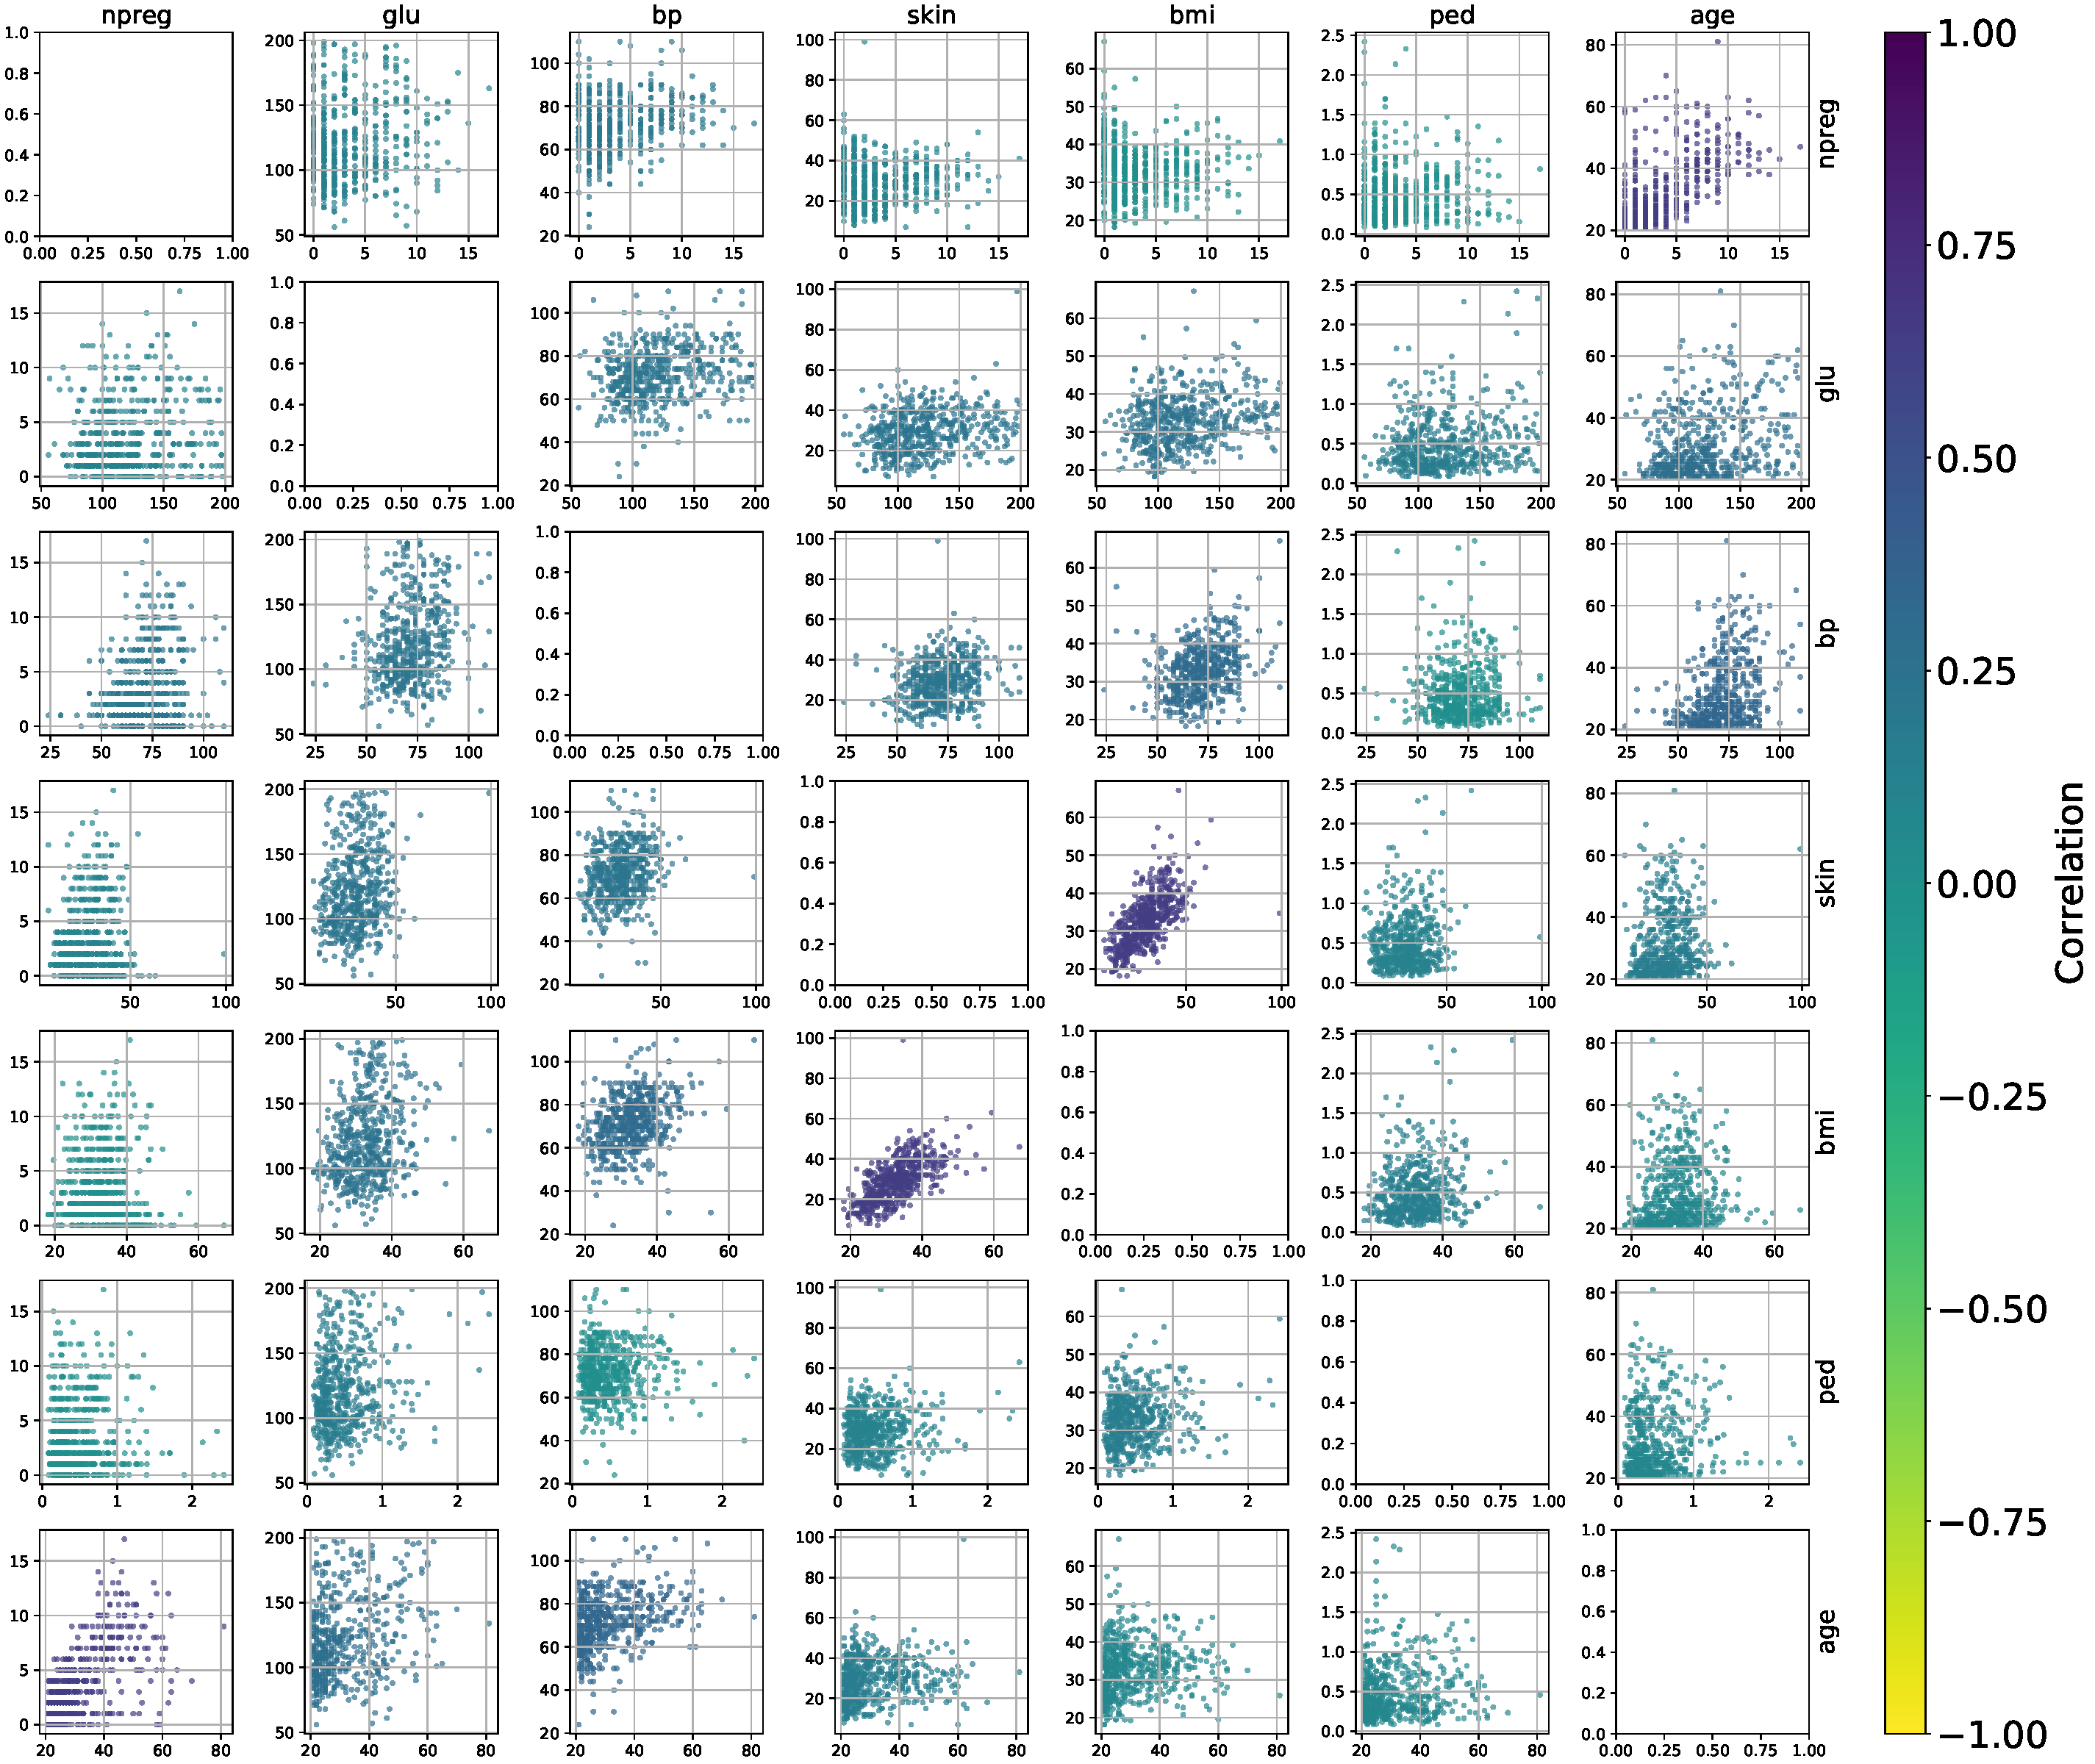
\includegraphics[width = 1.0\textwidth]{1-correlation.pdf}
    \caption{Gráfica de correlación para las variables numericas del problema 1}
    \label{1-correlation}
\end{figure}
\begin{figure}[H]
    \centering
    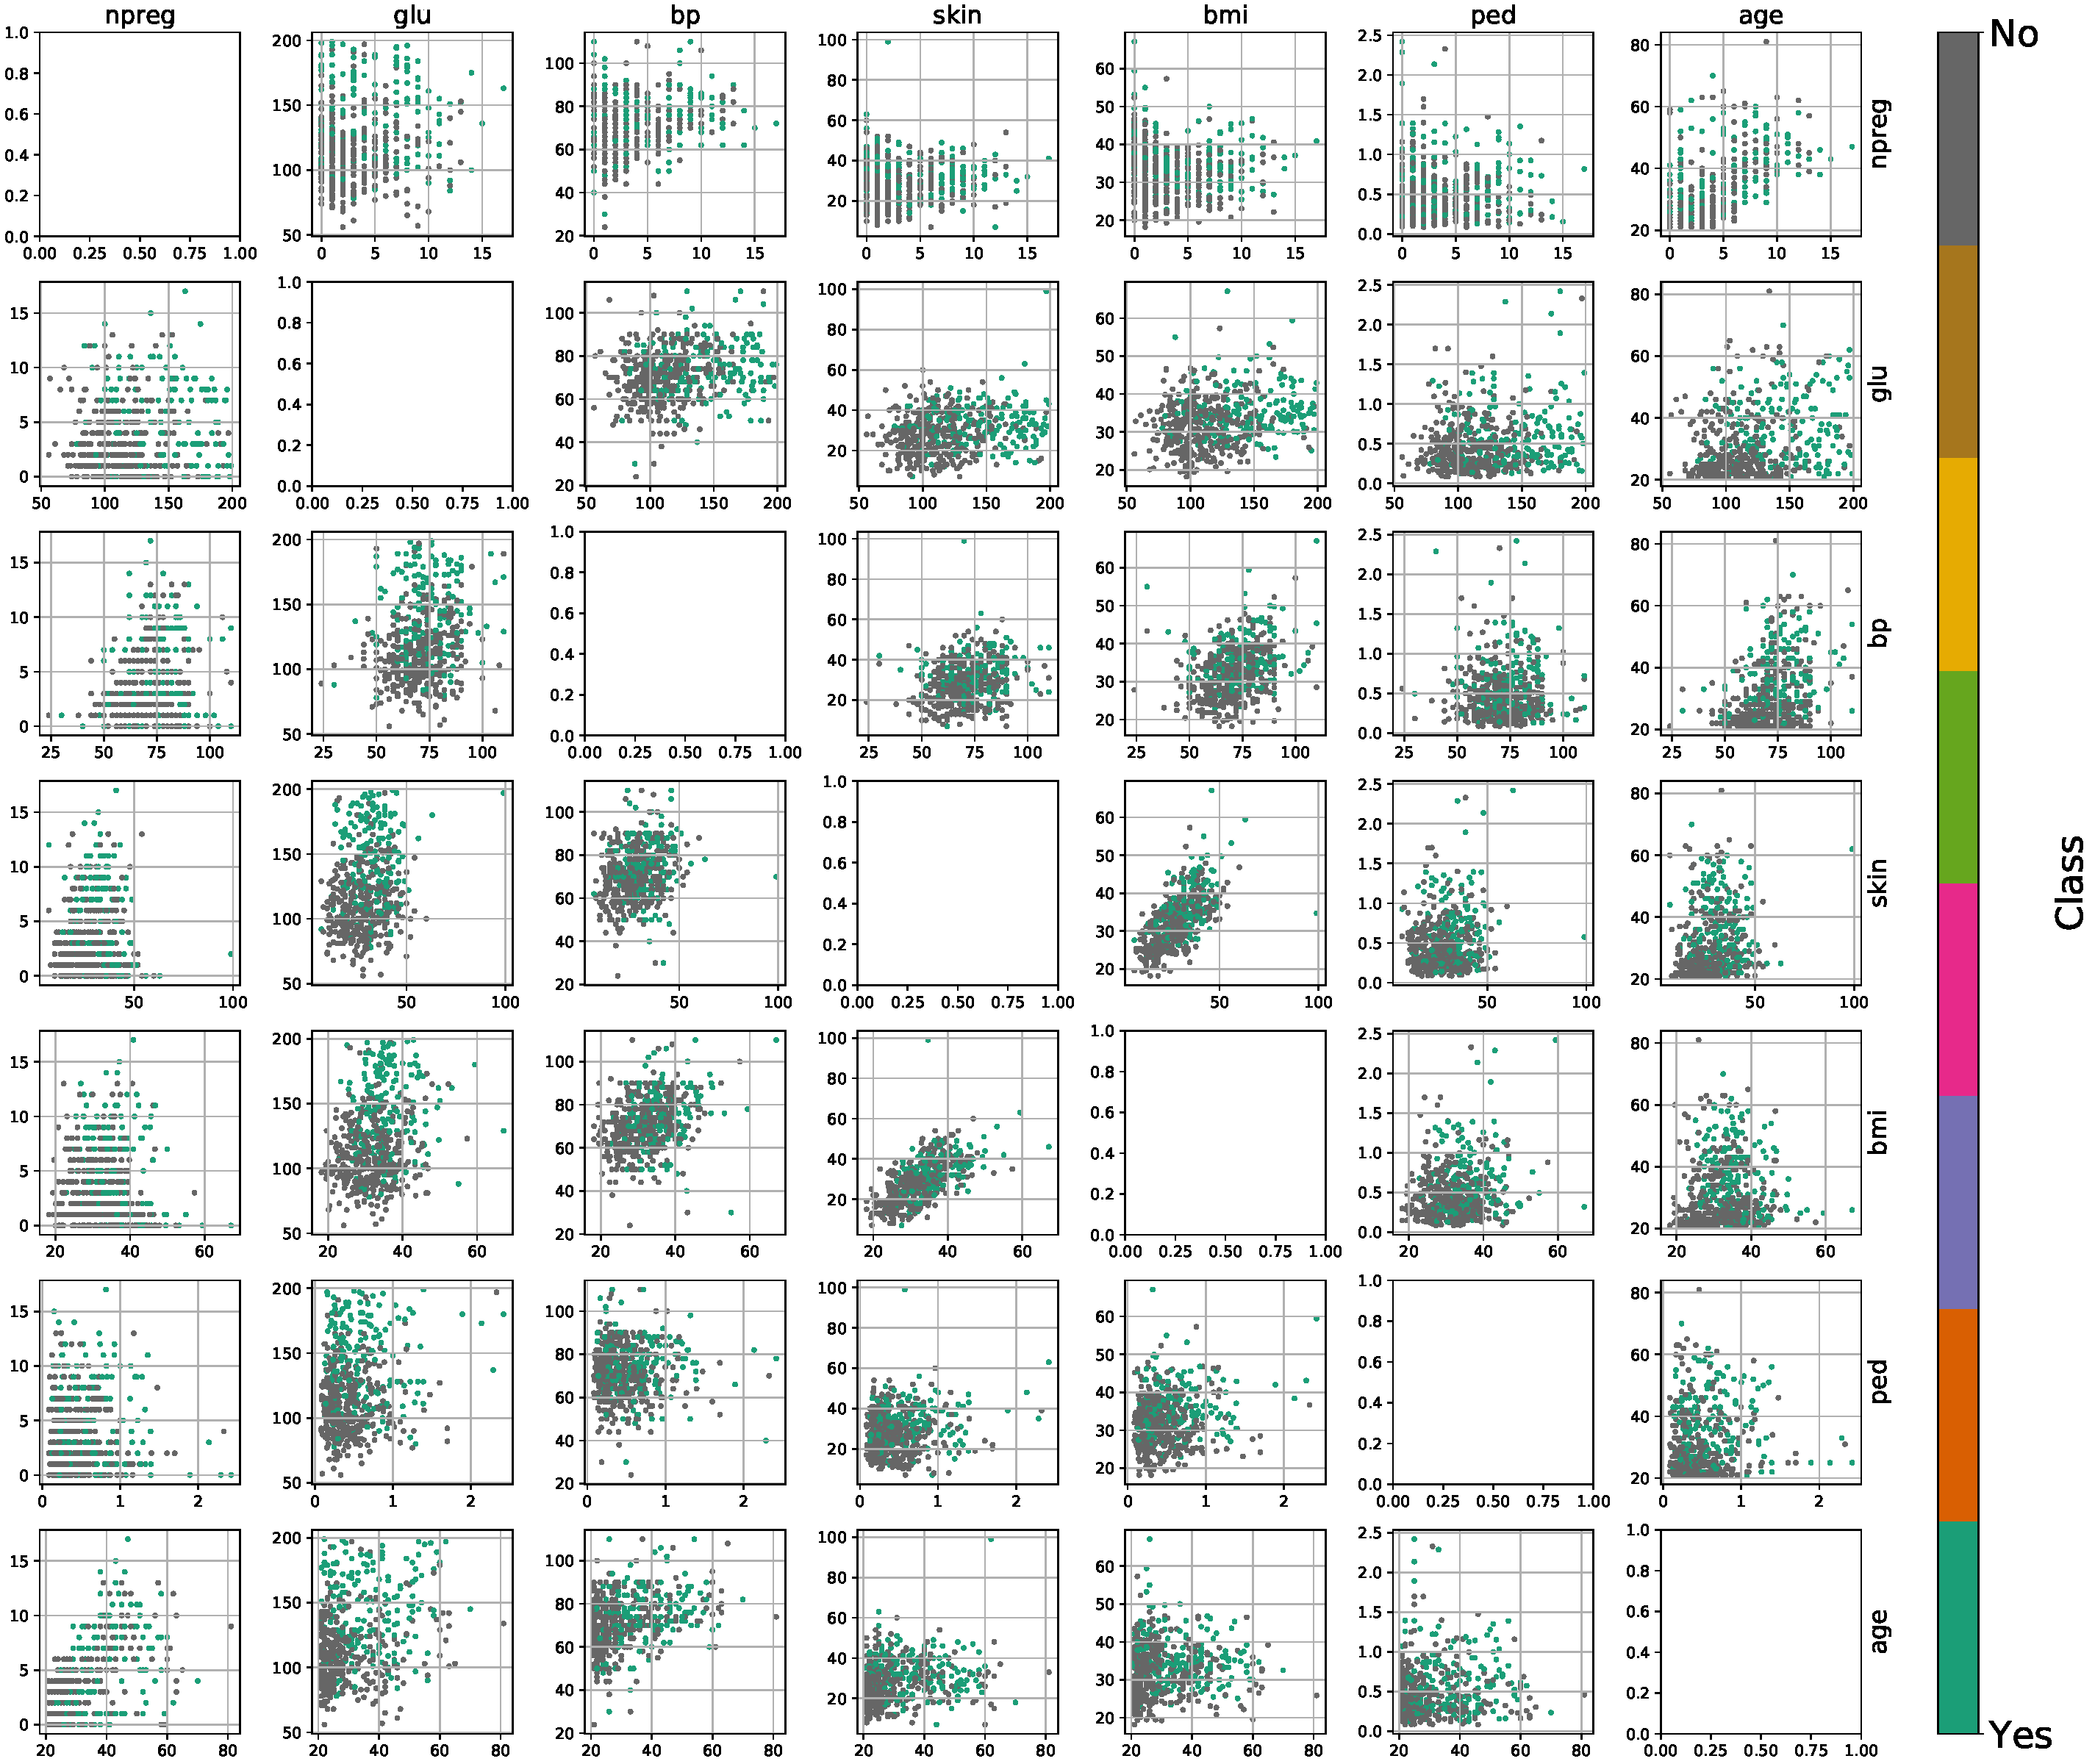
\includegraphics[width = 1.0\textwidth]{1-classes.pdf}
    \caption{Gráficas de una variable contra otra divididas en clases para las variables numéricas del problema 1}
    \label{1-classes}
\end{figure}
\begin{figure}[H]
    \centering
    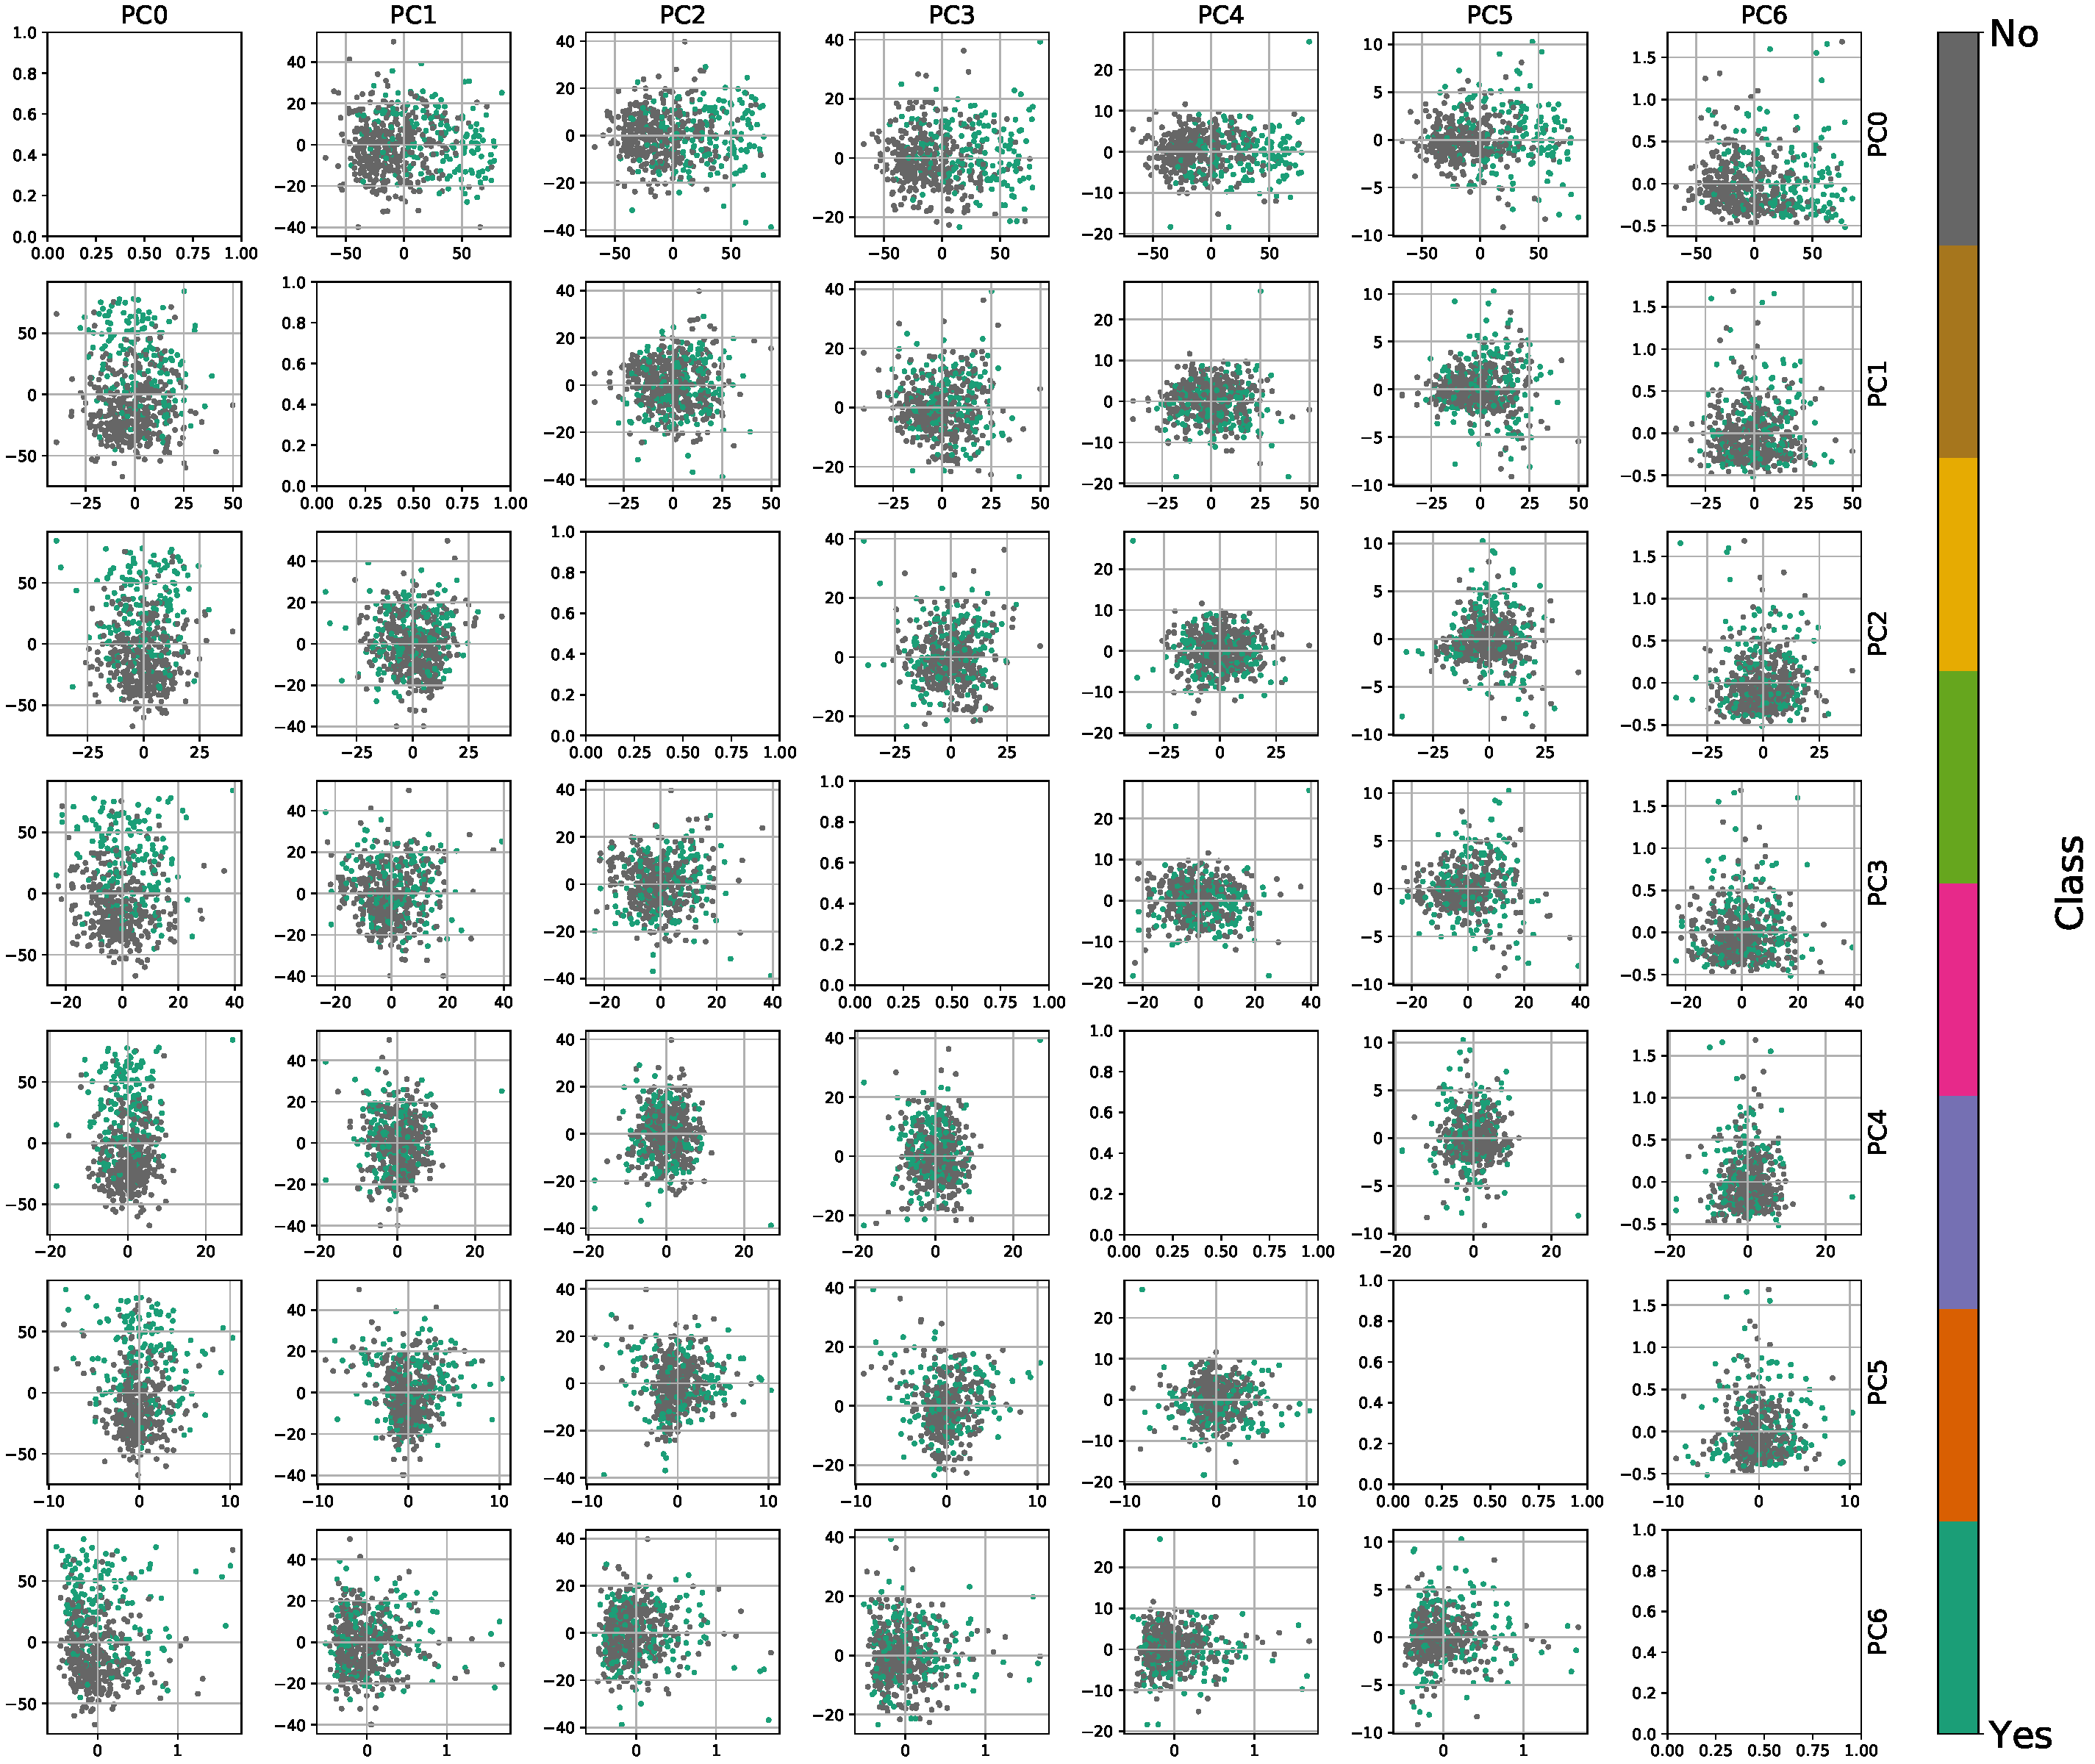
\includegraphics[width = 1.0\textwidth]{1-pca.pdf}
    \caption{Gráficas de una variable contra otra divididas en clases para las componentes principales del problema 1}
    \label{1-pca}
\end{figure}
\begin{figure}[H]
    \centering
    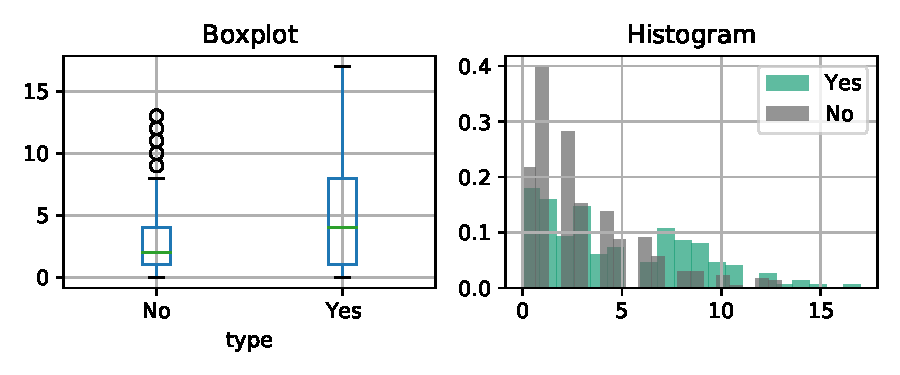
\includegraphics[width = 0.65\textwidth]{1-npreg-dist.pdf}
    \caption{Distribución de la variable ``npreg''}
    \label{1-npreg-dist}
\end{figure}
\begin{figure}[H]
    \centering
    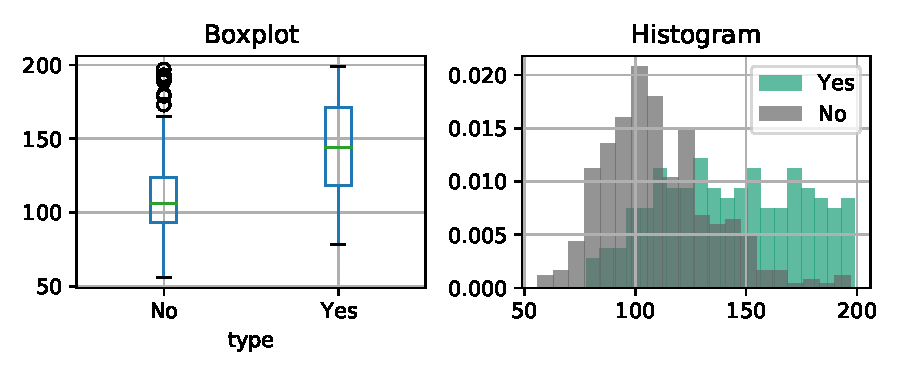
\includegraphics[width = 0.65\textwidth]{1-glu-dist.pdf}
    \caption{Distribución de la variable ``glu''}
    \label{1-glu-dist}
\end{figure}
\begin{figure}[H]
    \centering
    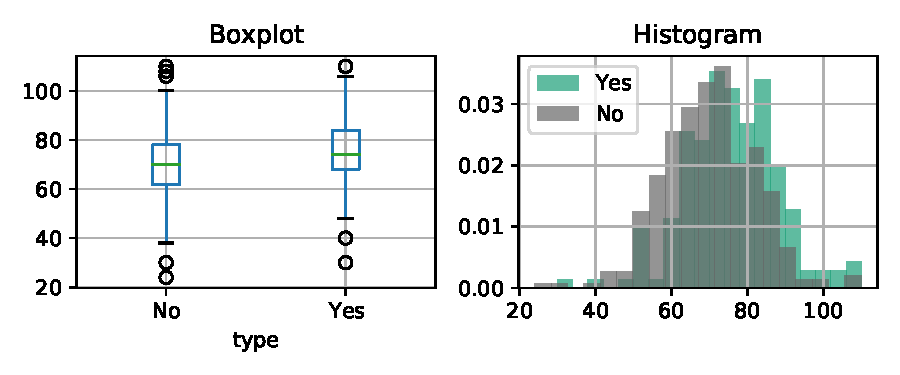
\includegraphics[width = 0.65\textwidth]{1-bp-dist.pdf}
    \caption{Distribución de la variable ``bp''}
    \label{1-bp-dist}
\end{figure}
\begin{figure}[H]
    \centering
    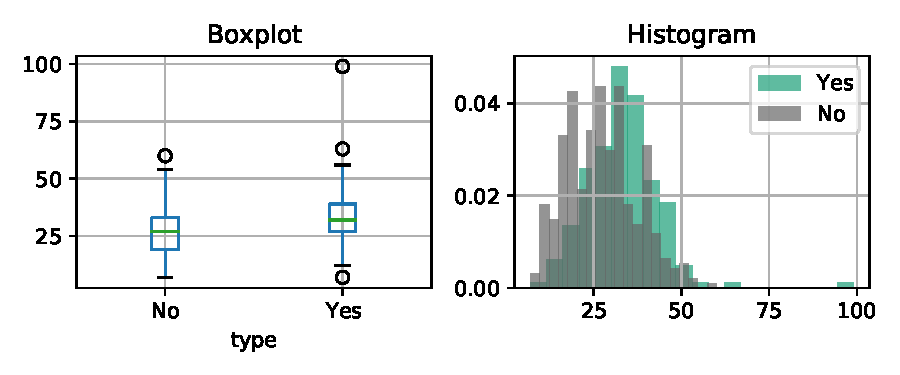
\includegraphics[width = 0.65\textwidth]{1-skin-dist.pdf}
    \caption{Distribución de la variable ``skin''}
    \label{1-skin-dist}
\end{figure}
\begin{figure}[H]
    \centering
    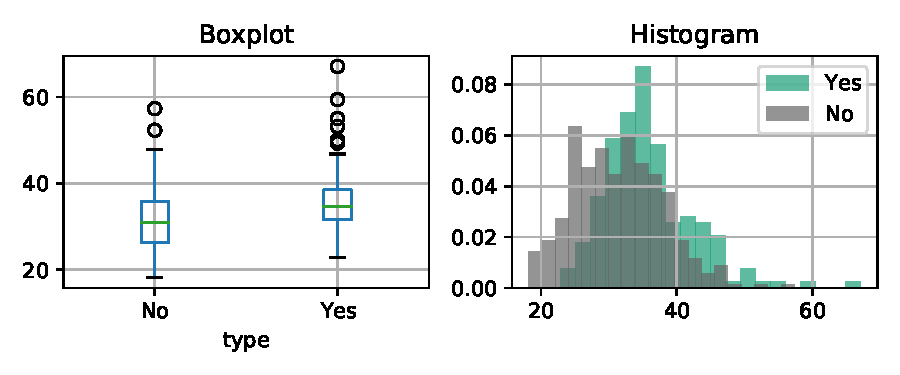
\includegraphics[width = 0.65\textwidth]{1-bmi-dist.pdf}
    \caption{Distribución de la variable ``bmi''}
    \label{1-bmi-dist}
\end{figure}
\begin{figure}[H]
    \centering
    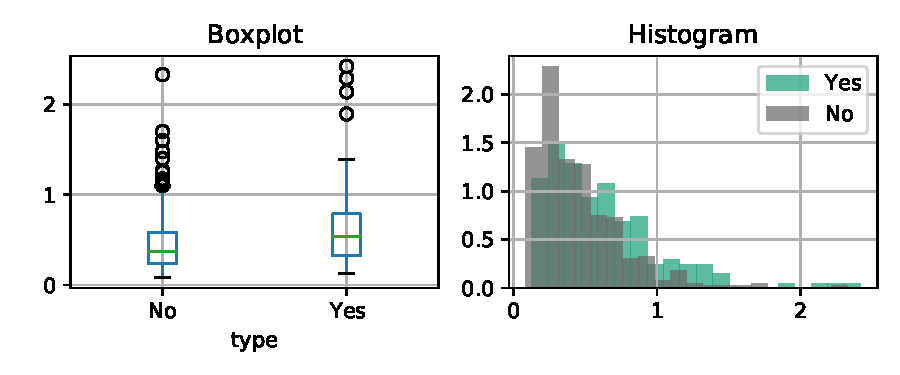
\includegraphics[width = 0.65\textwidth]{1-ped-dist.pdf}
    \caption{Distribución de la variable ``ped''}
    \label{1-ped-dist}
\end{figure}
\begin{figure}[H]
    \centering
    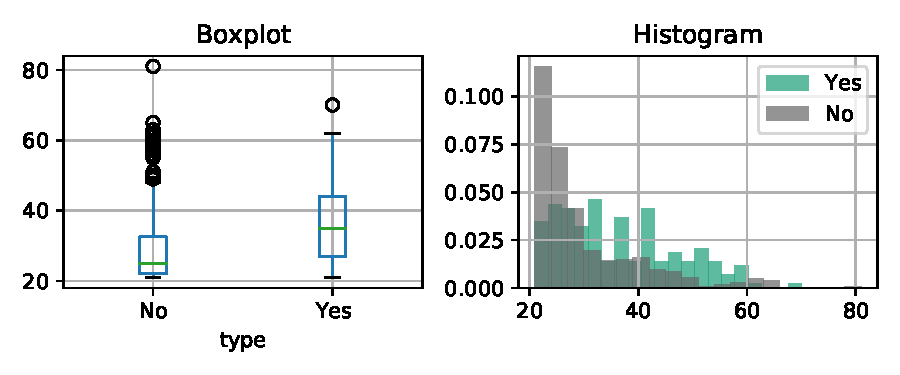
\includegraphics[width = 0.65\textwidth]{1-age-dist.pdf}
    \caption{Distribución de la variable ``age''}
    \label{1-age-dist}
\end{figure}
\begin{figure}[H]
    \centering
    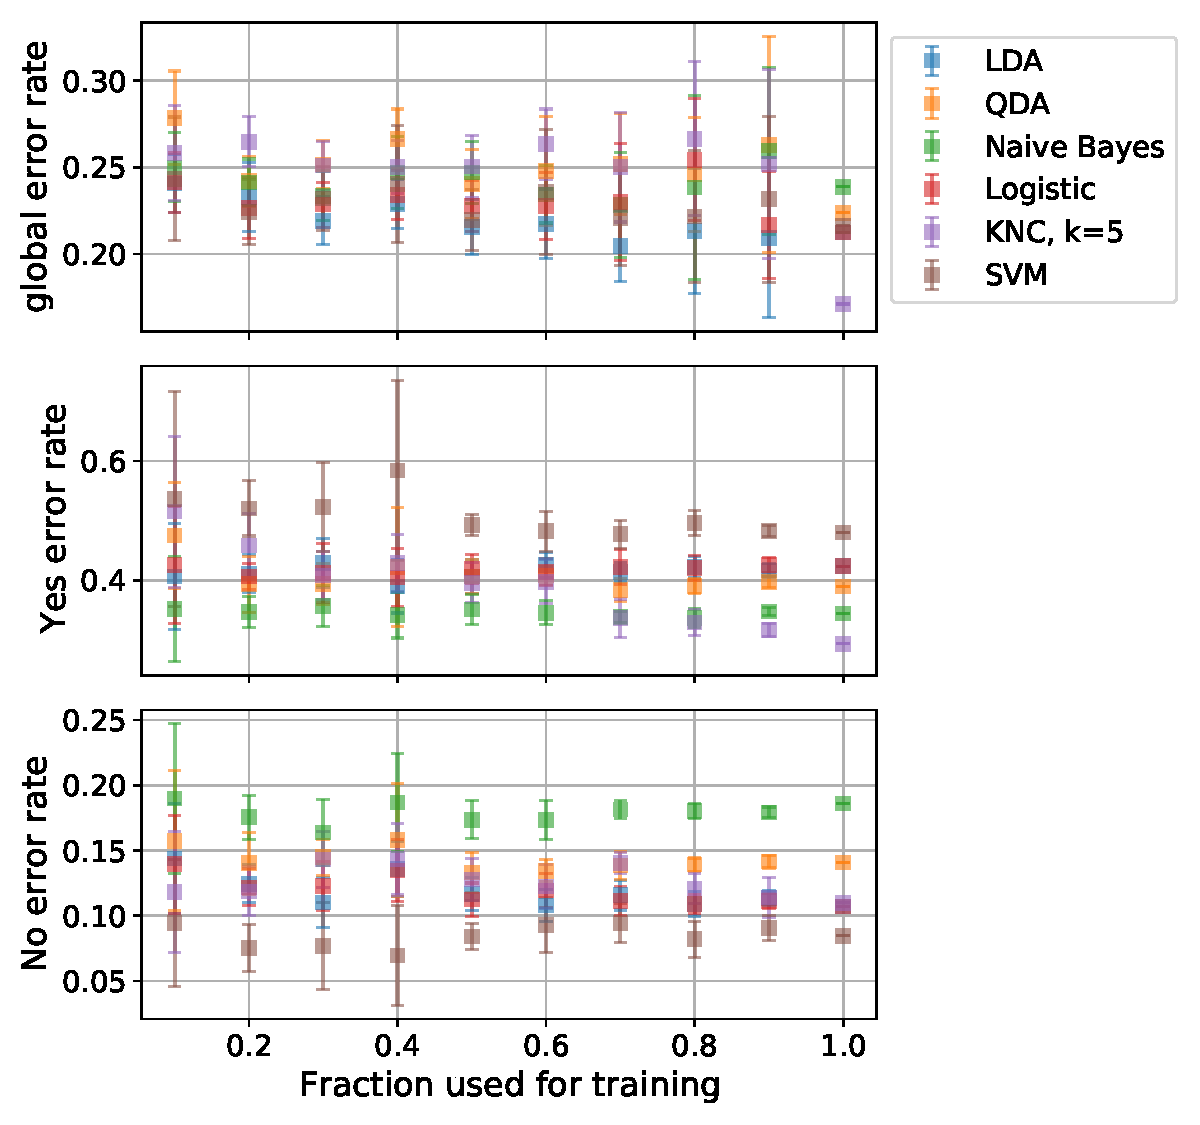
\includegraphics[width = 0.8\textwidth]{1-gen-sizeDependence.pdf}
    \caption{Tasas globales y locales para varios modelos, con conjuntos de entrenamiento divididos sin mantener proporcionalidad}
    \label{1-gen-sizeDependence}
\end{figure}
\begin{figure}[H]
    \centering
    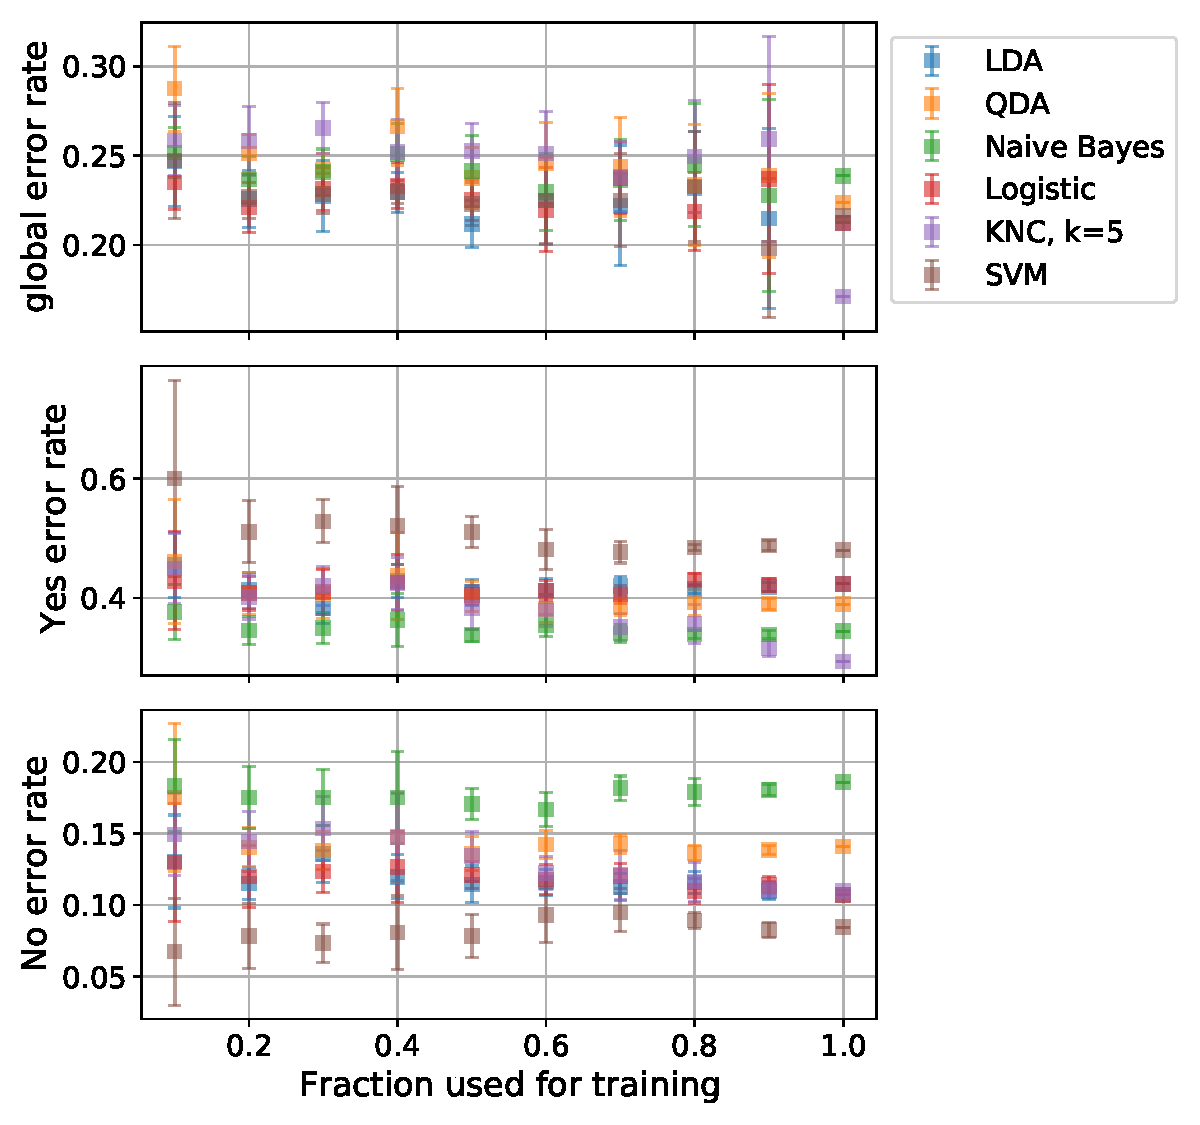
\includegraphics[width = 0.8\textwidth]{1-gen-eq-sizeDependence.pdf}
    \caption{Tasas globales y locales para varios modelos, con conjuntos de entrenamiento divididos manteniendo proporcionalidad}
    \label{1-gen-eq-sizeDependence}
\end{figure}
\begin{figure}[H]
    \centering
    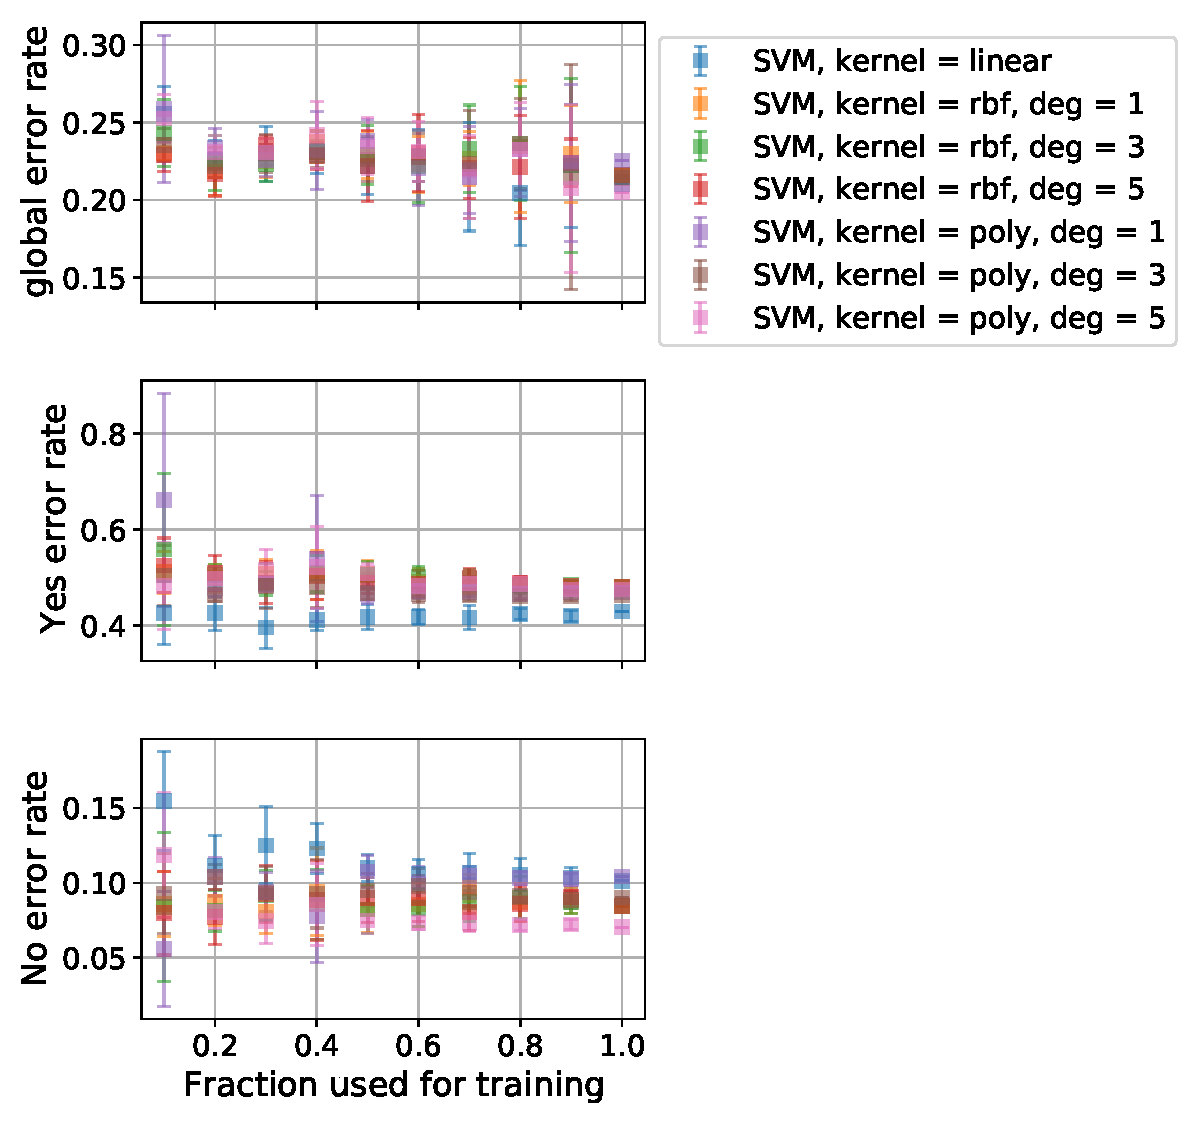
\includegraphics[width = 0.8\textwidth]{1-svm-eq-sizeDependence.pdf}
    \caption{Tasas globales y locales para modelos SVM, con conjuntos de entrenamiento divididos manteniendo proporcionalidad}
    \label{1-svm-eq-sizeDependence}
\end{figure}
\begin{figure}[H]
    \centering
    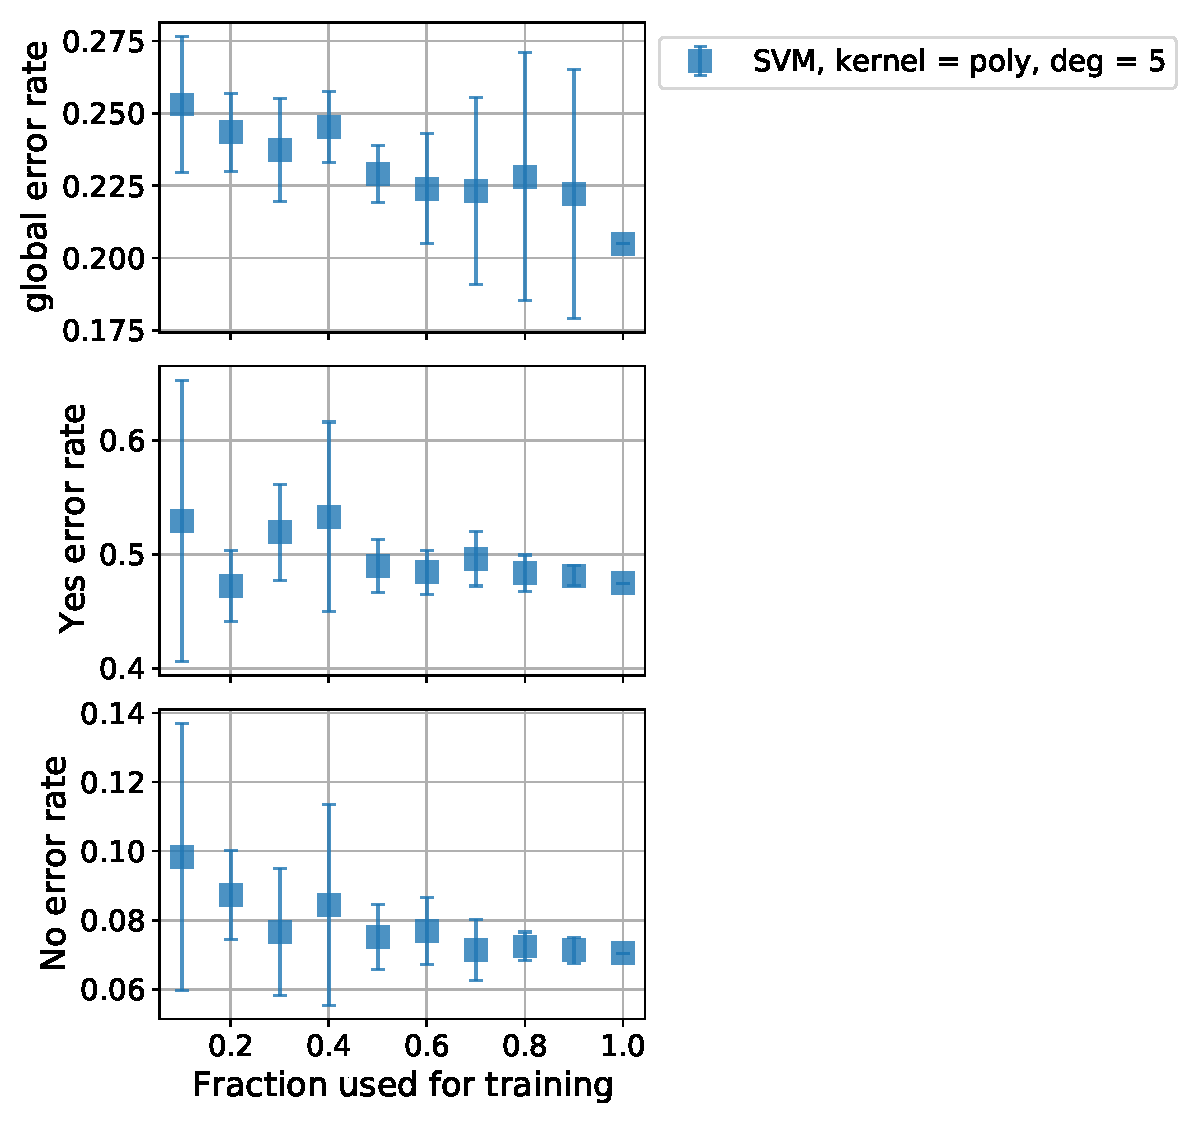
\includegraphics[width = 0.8\textwidth]{1-svm-fin-eq-sizeDependence.pdf}
    \caption{Tasas globales y locales para modelos SVM, con conjuntos de entrenamiento divididos manteniendo proporcionalidad}
    \label{1-svm-fin-eq-sizeDependence}
\end{figure}
\begin{figure}[H]
    \centering
    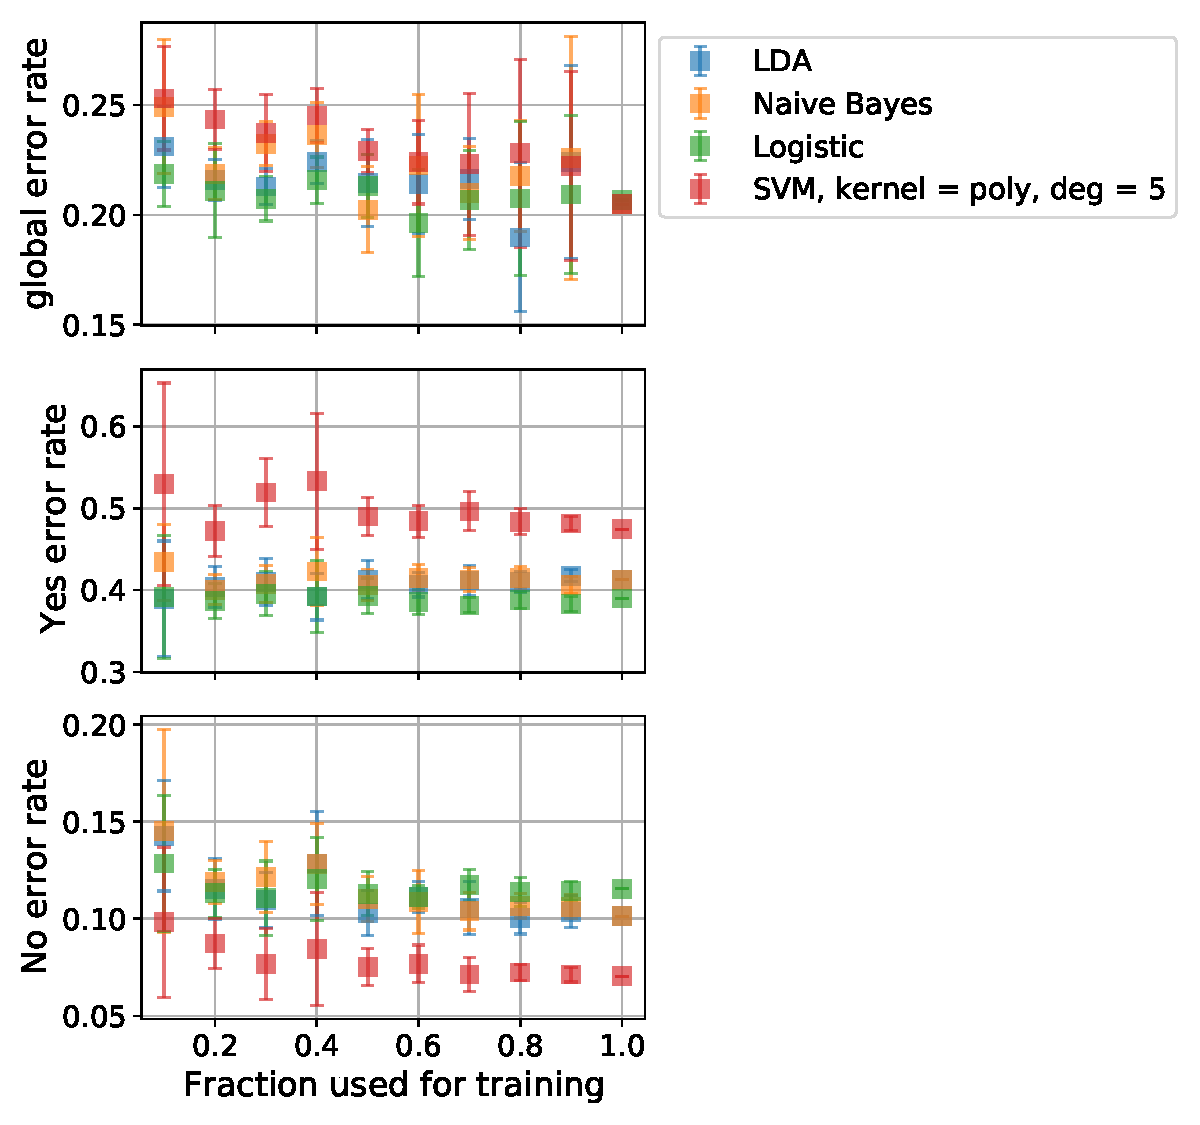
\includegraphics[width = 0.8\textwidth]{1-final-sizeDependence.pdf}
    \caption{Tasas globales y locales para modelos SVM, con conjuntos de entrenamiento divididos manteniendo proporcionalidad}
    \label{1-final-sizeDependence}
\end{figure}
\subsection*{Problema 2}
\begin{figure}[H]
    \centering
    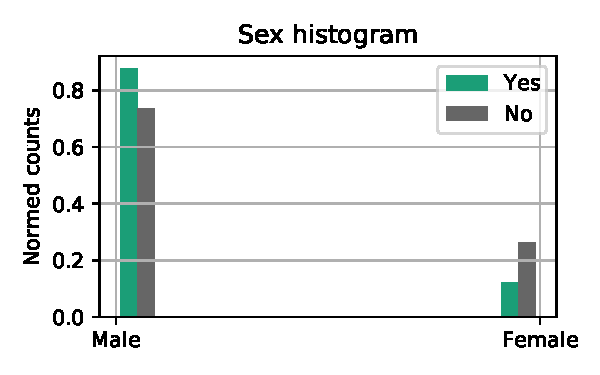
\includegraphics[width = 0.65\textwidth]{2-Sex-dist.pdf}
    \caption{Distribución de la variable ``Sex''}
    \label{2-Sex-dist}
\end{figure}
\begin{figure}[H]
    \centering
    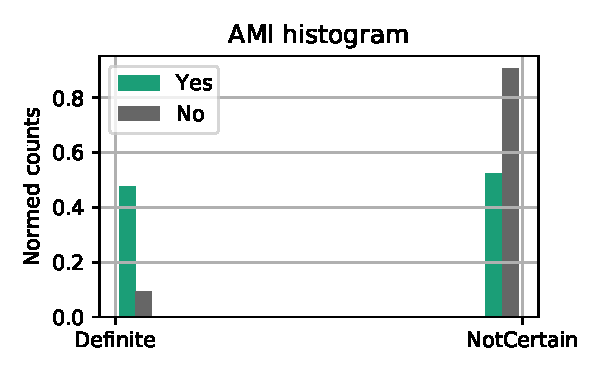
\includegraphics[width = 0.65\textwidth]{2-AMI-dist.pdf}
    \caption{Distribución de la variable ``AngPec''}
    \label{2-AMI-dist}
\end{figure}
\begin{figure}[H]
    \centering
    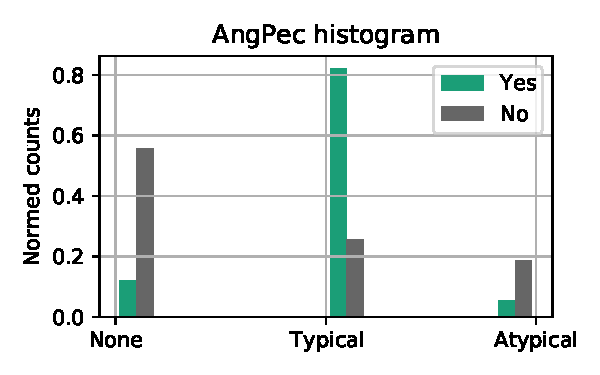
\includegraphics[width = 0.65\textwidth]{2-AngPec-dist.pdf}
    \caption{Distribución de la variable ``AngPec''}
    \label{2-AngPec-dist}
\end{figure}
\begin{figure}[H]
    \centering
    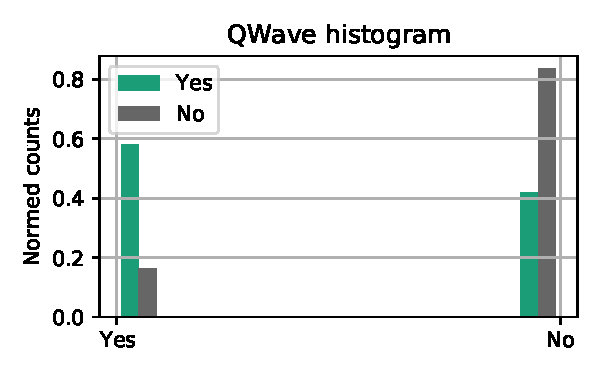
\includegraphics[width = 0.65\textwidth]{2-QWave-dist.pdf}
    \caption{Distribución de la variable ``QWave''}
    \label{2-QWave-dist}
\end{figure}
\begin{figure}[H]
    \centering
    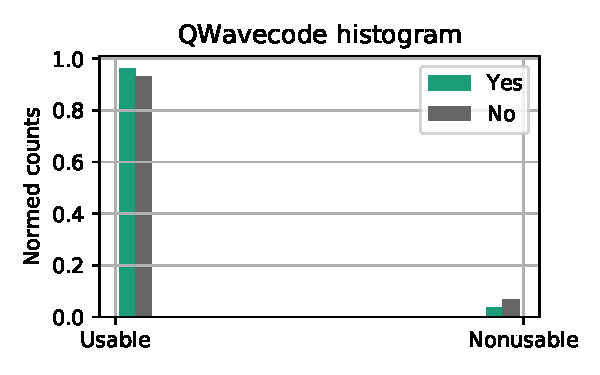
\includegraphics[width = 0.65\textwidth]{2-QWavecode-dist.pdf}
    \caption{Distribución de la variable ``QWavecode''}
    \label{2-QWavecode-dist}
\end{figure}
\begin{figure}[H]
    \centering
    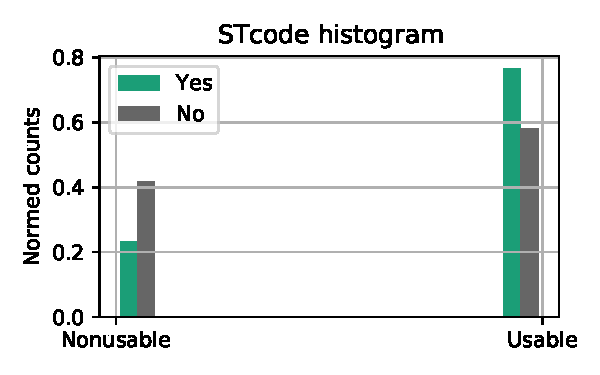
\includegraphics[width = 0.65\textwidth]{2-STcode-dist.pdf}
    \caption{Distribución de la variable ``STcode''}
    \label{2-STcode-dist}
\end{figure}
\begin{figure}[H]
    \centering
    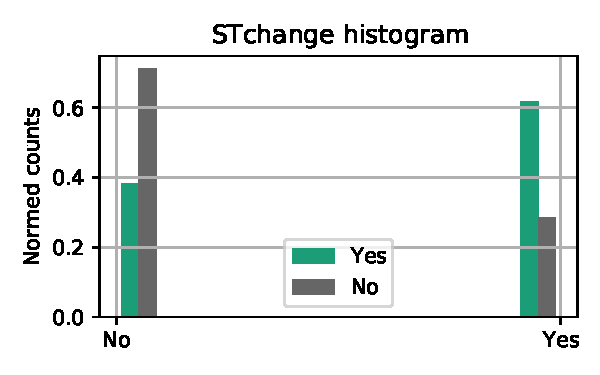
\includegraphics[width = 0.65\textwidth]{2-STchange-dist.pdf}
    \caption{Distribución de la variable ``STchange''}
    \label{2-STchange-dist}
\end{figure}
\begin{figure}[H]
    \centering
    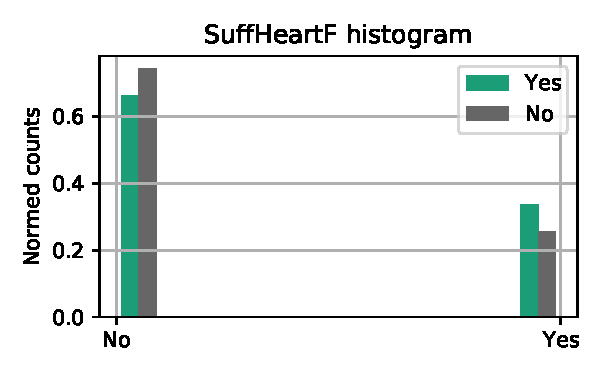
\includegraphics[width = 0.65\textwidth]{2-SuffHeartF-dist.pdf}
    \caption{Distribución de la variable ``SuffHeartF''}
    \label{2-SuffHeartF-dist}
\end{figure}
\begin{figure}[H]
    \centering
    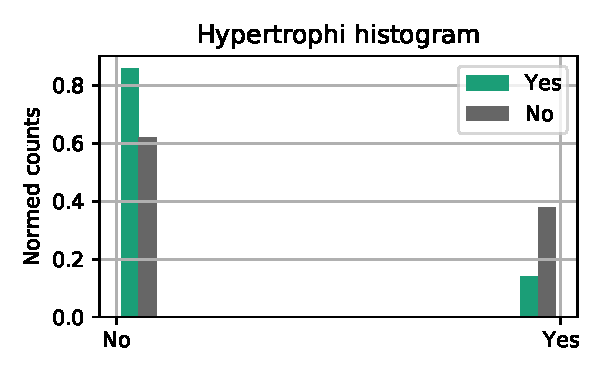
\includegraphics[width = 0.65\textwidth]{2-Hypertrophi-dist.pdf}
    \caption{Distribución de la variable ``Hypertrophi''}
    \label{2-Hypertrophi-dist}
\end{figure}
\begin{figure}[H]
    \centering
    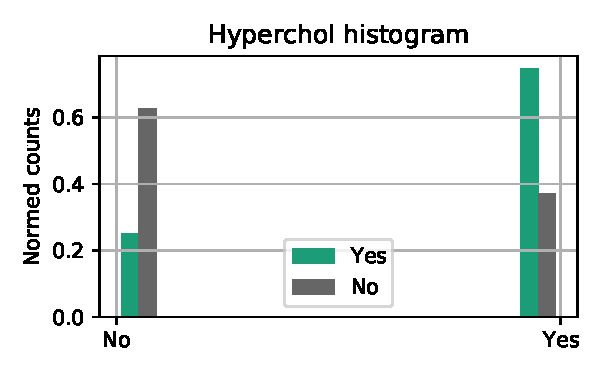
\includegraphics[width = 0.65\textwidth]{2-Hyperchol-dist.pdf}
    \caption{Distribución de la variable ``Hyperchol''}
    \label{2-Hyperchol-dist}
\end{figure}
\begin{figure}[H]
    \centering
    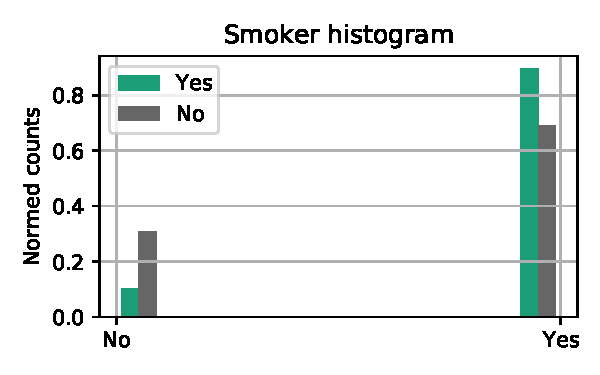
\includegraphics[width = 0.65\textwidth]{2-Smoker-dist.pdf}
    \caption{Distribución de la variable ``Smoker''}
    \label{2-Smoker-dist}
\end{figure}
\begin{figure}[H]
    \centering
    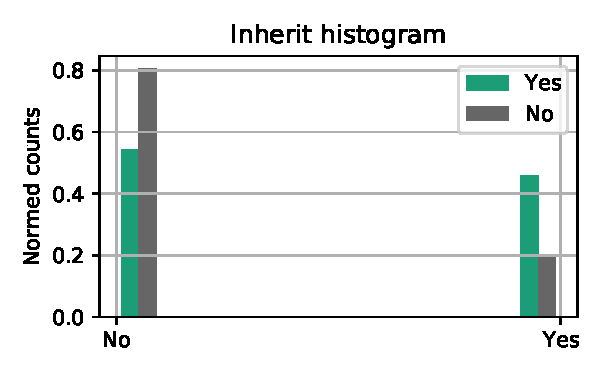
\includegraphics[width = 0.65\textwidth]{2-Inherit-dist.pdf}
    \caption{Distribución de la variable ``Inherit''}
    \label{2-Inherit-dist}
\end{figure}
\begin{figure}[H]
    \centering
    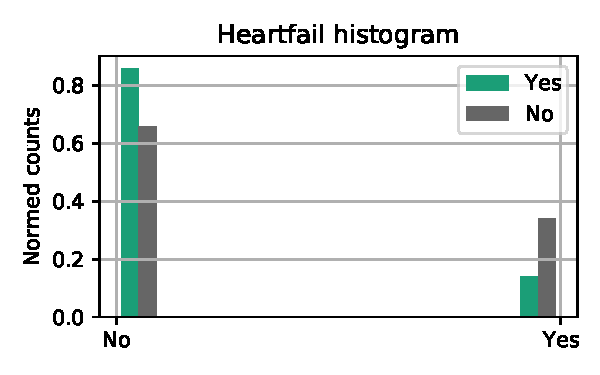
\includegraphics[width = 0.65\textwidth]{2-Heartfail-dist.pdf}
    \caption{Distribución de la variable ``Heartfail''}
    \label{2-Heartfail-dist}
\end{figure}
\begin{figure}[H]
    \centering
    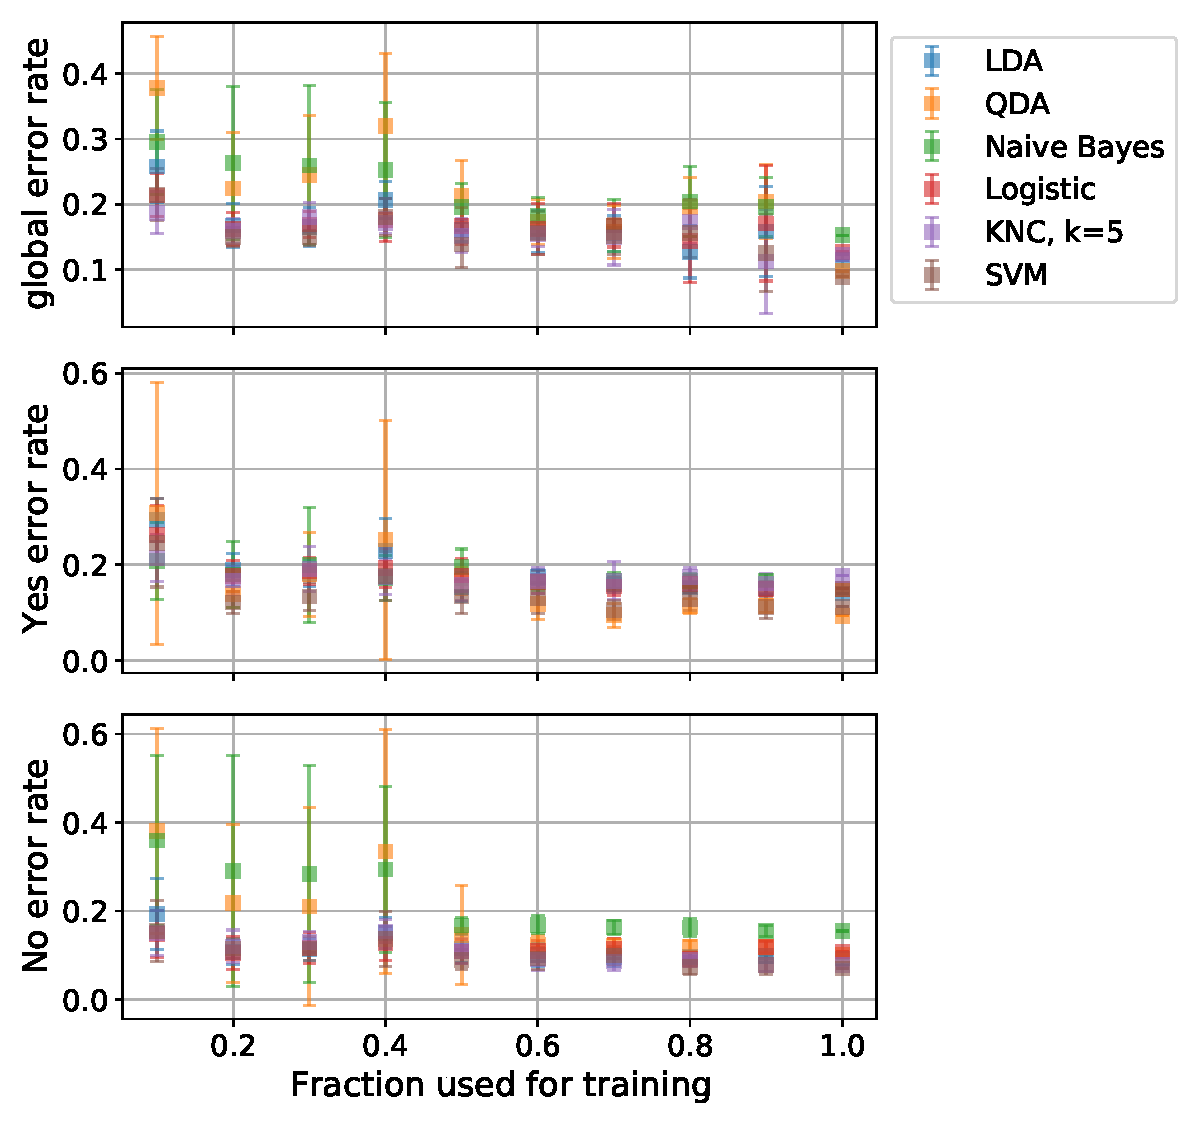
\includegraphics[width = 0.8\textwidth]{2-gen-eq-sizeDependence.pdf}
    \caption{Tasas globales y locales para varios modelos, con conjuntos de entrenamiento divididos manteniendo proporcionalidad}
    \label{2-gen-eq-sizeDependence}
\end{figure}
\begin{figure}[H]
    \centering
    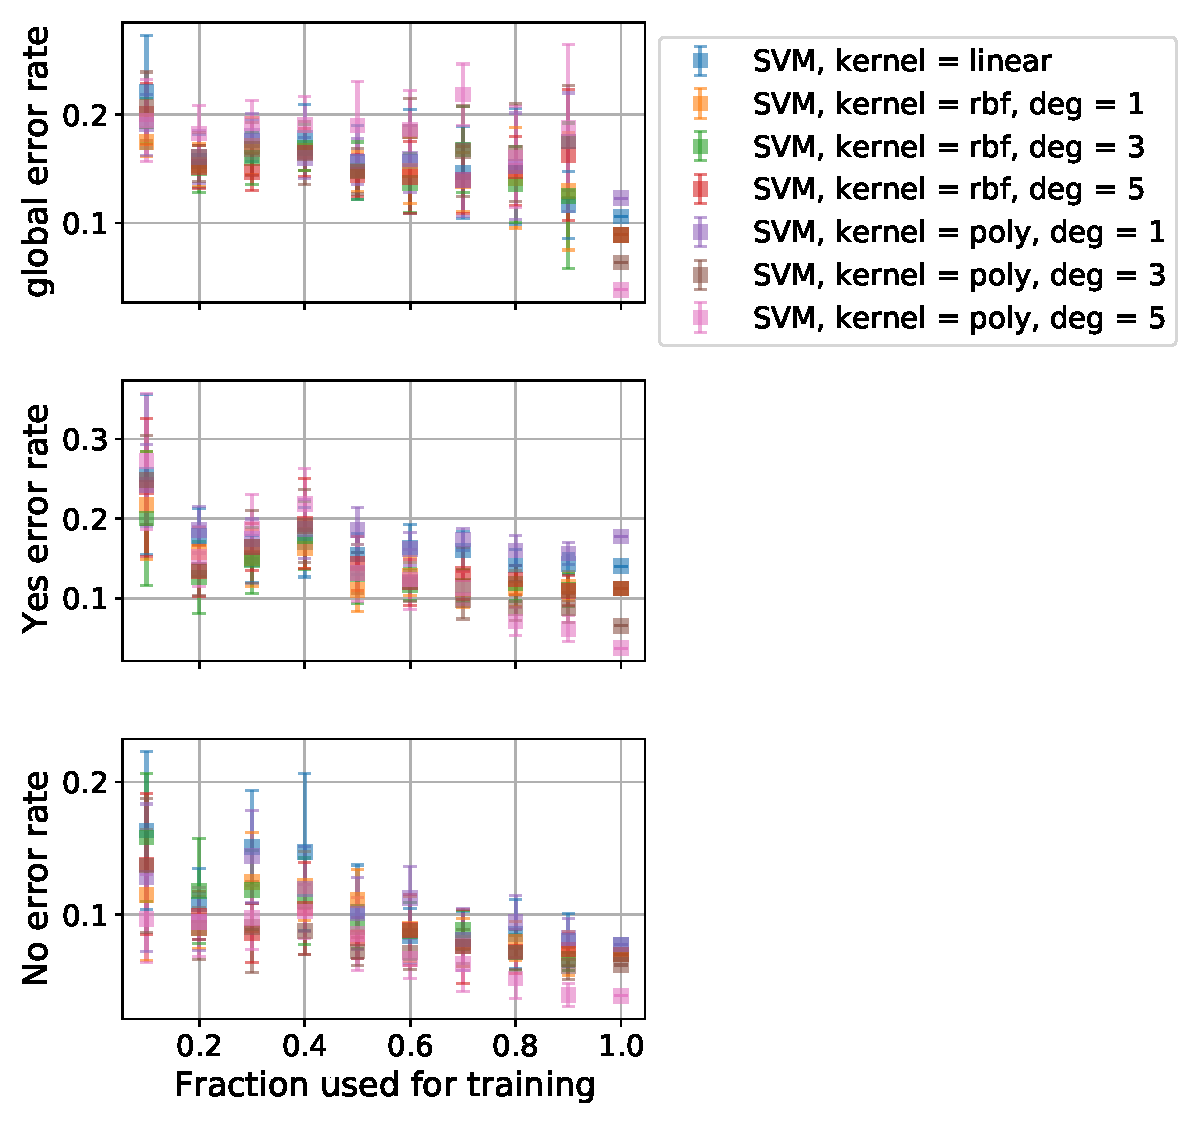
\includegraphics[width = 0.8\textwidth]{2-svm-eq-sizeDependence.pdf}
    \caption{Tasas globales y locales para modelos SVM, con conjuntos de entrenamiento divididos manteniendo proporcionalidad}
    \label{2-svm-eq-sizeDependence}
\end{figure}
\begin{figure}[H]
    \centering
    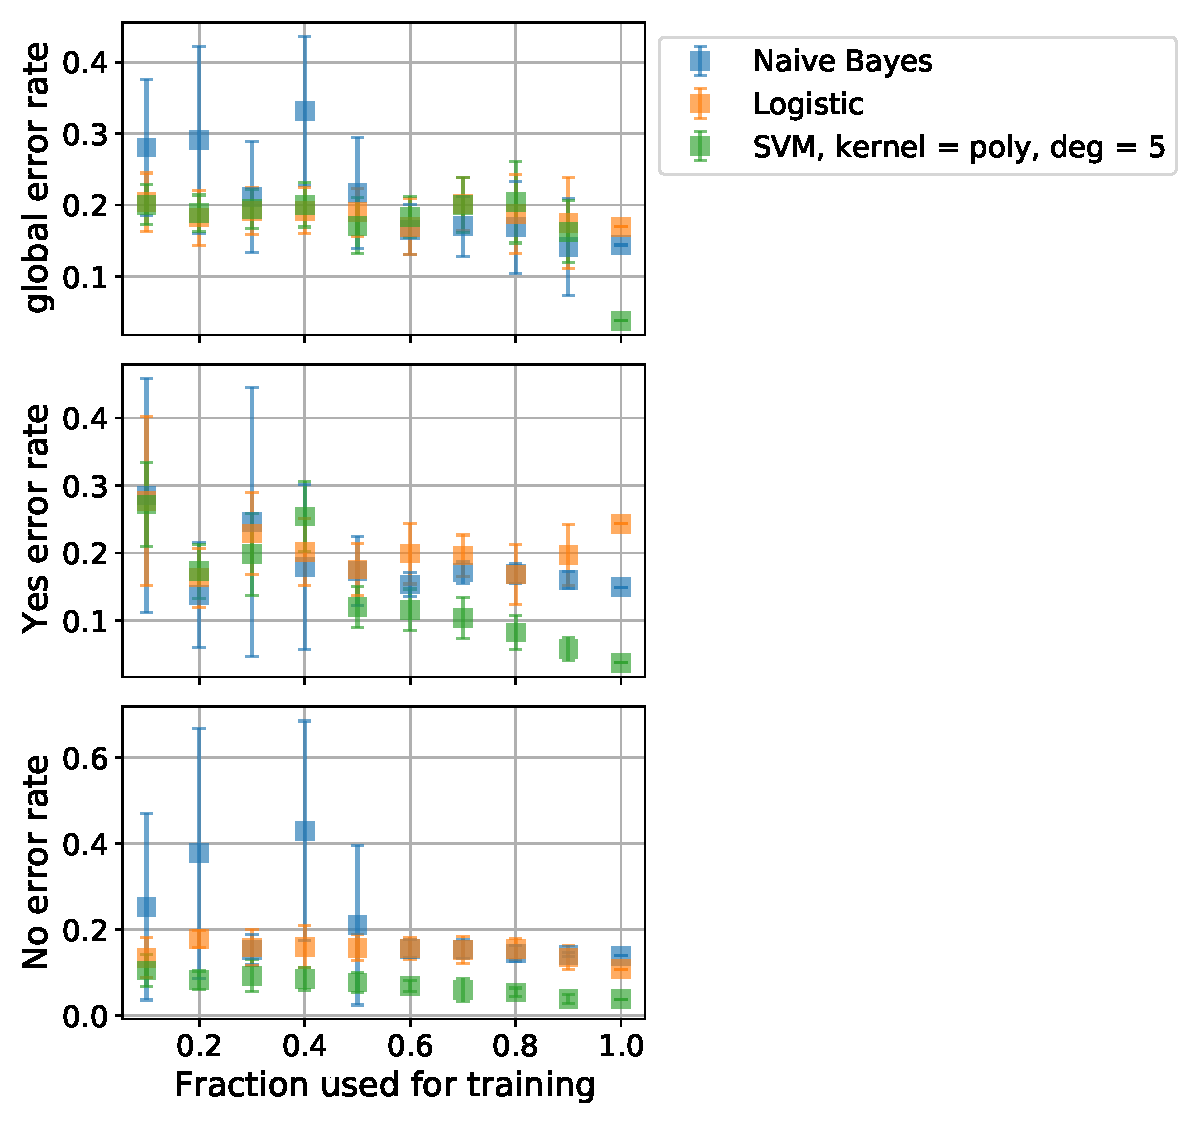
\includegraphics[width = 0.8\textwidth]{2-final-sizeDependence.pdf}
    \caption{Tasas globales y locales para modelos SVM, con conjuntos de entrenamiento divididos manteniendo proporcionalidad}
    \label{2-final-sizeDependence}
\end{figure}
\subsection*{Problema 3}
\begin{figure}[H]
    \centering
    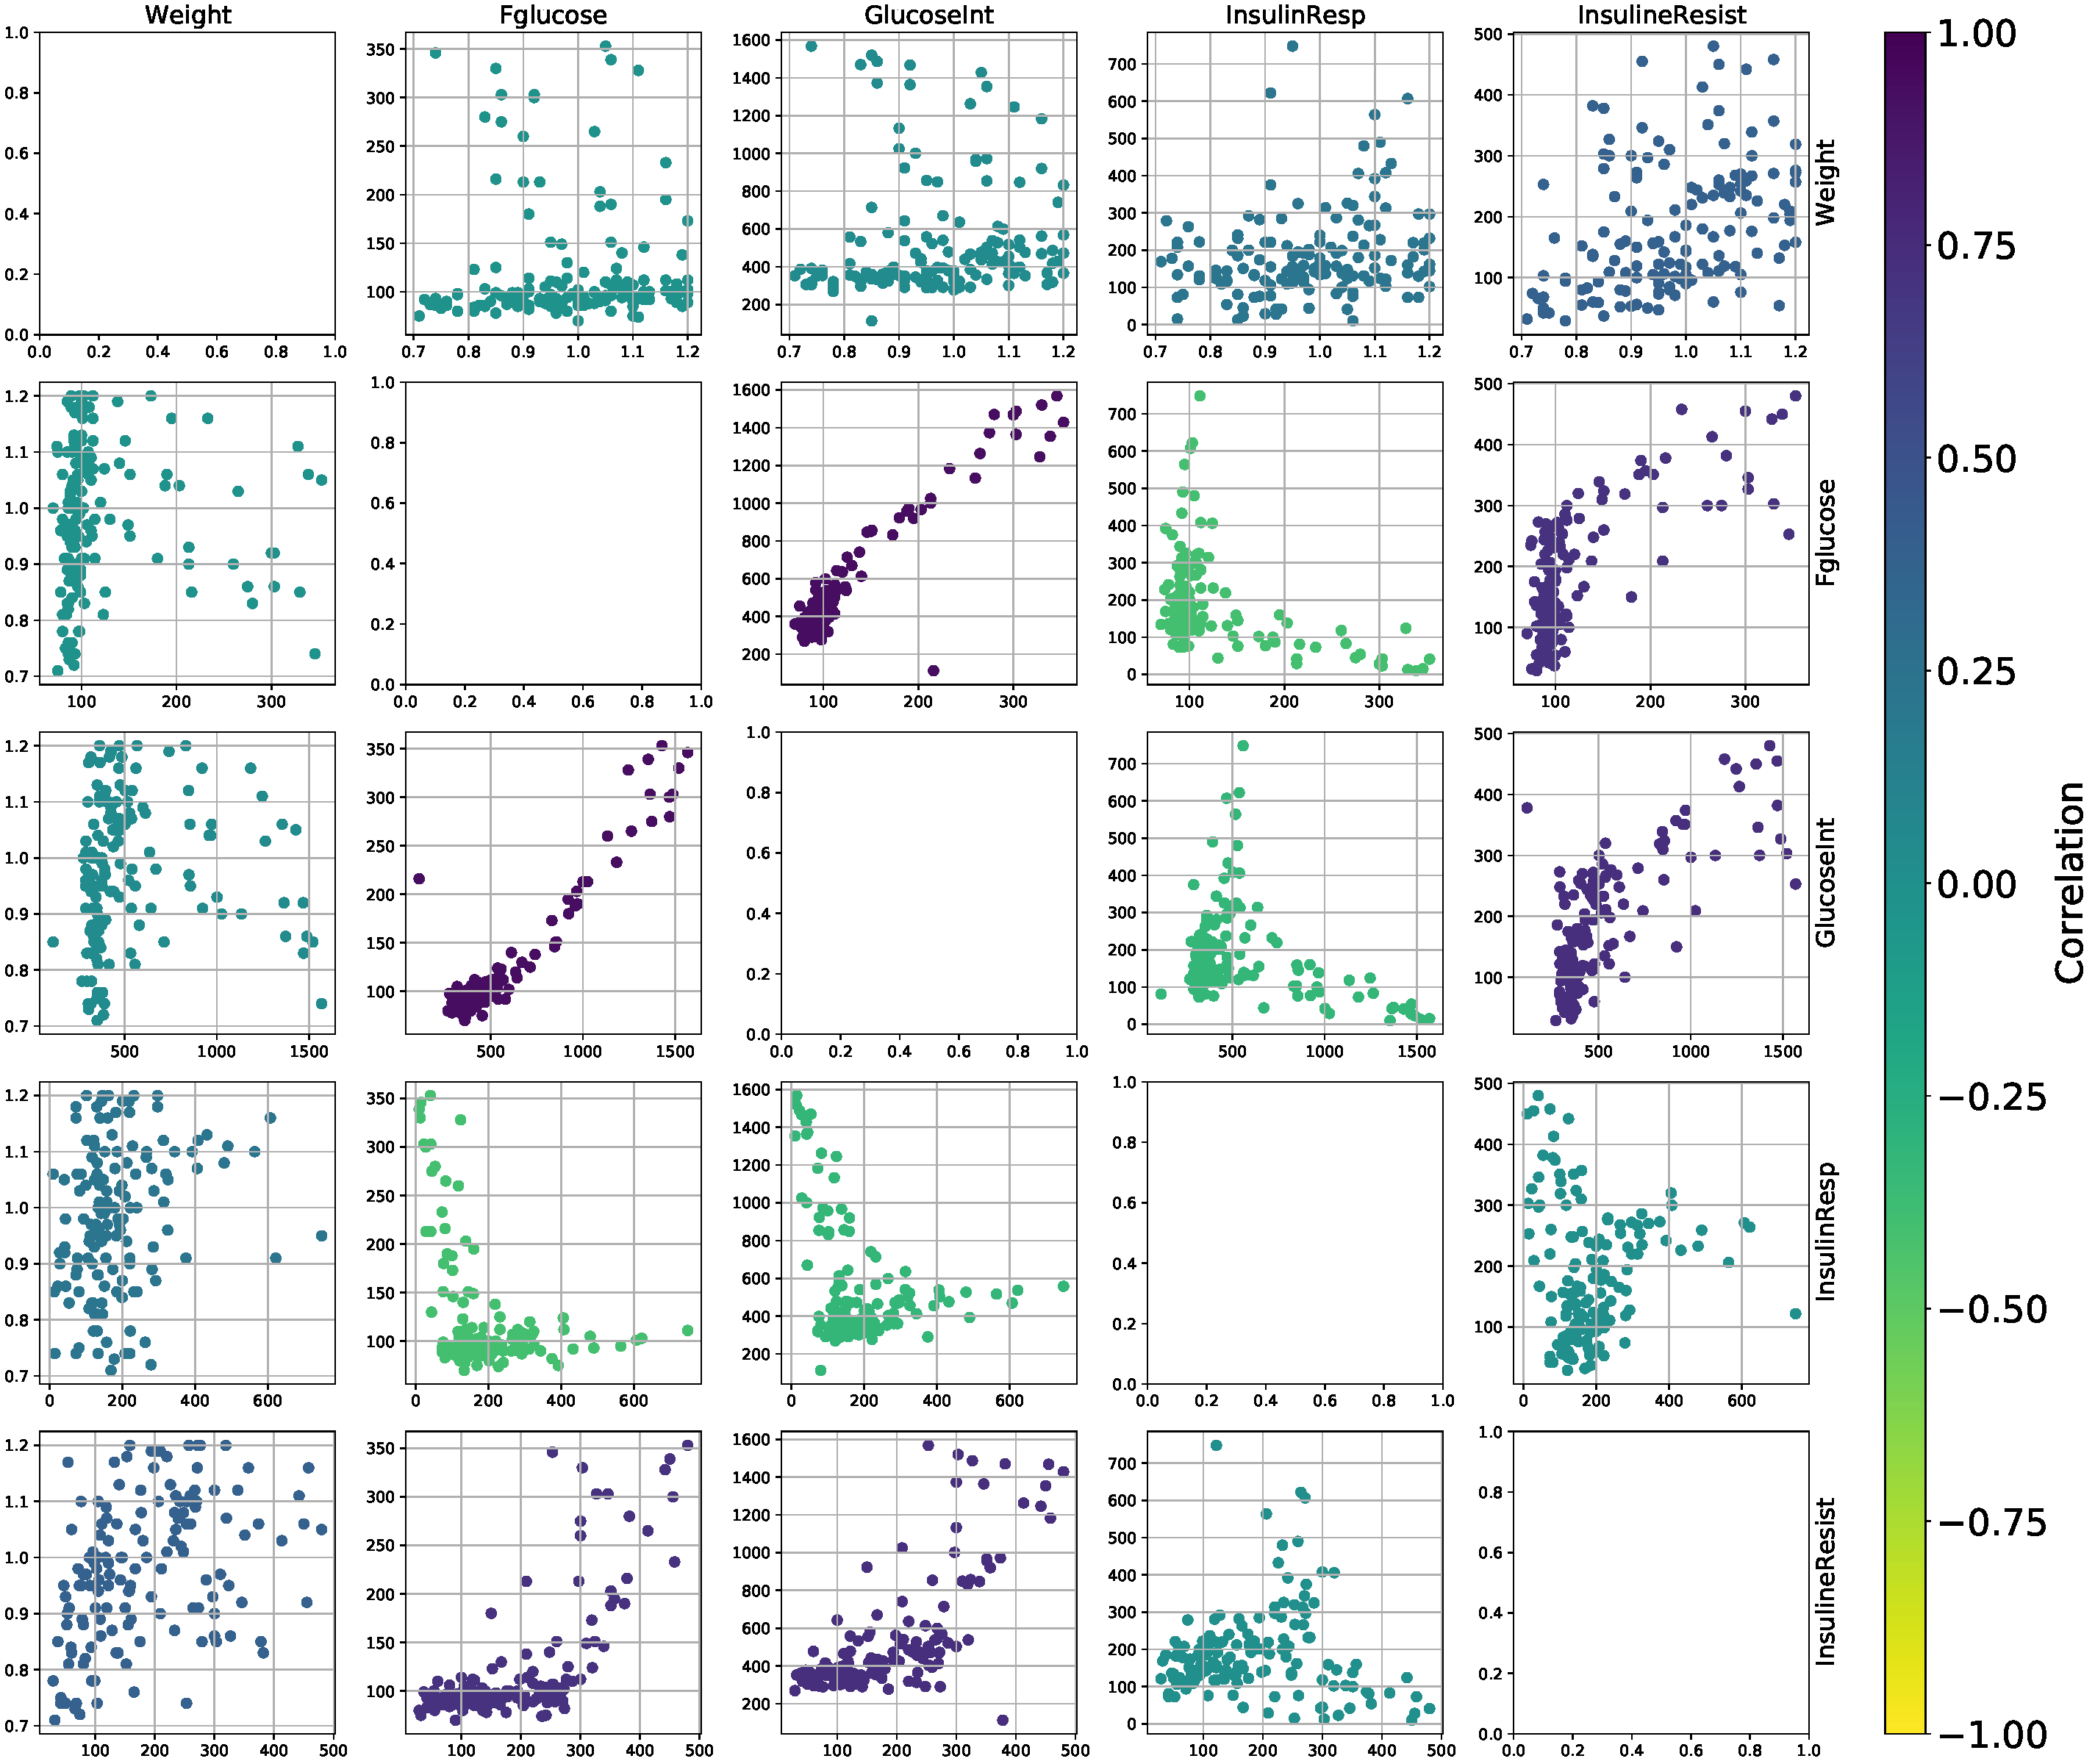
\includegraphics[width = 1.0\textwidth]{3-correlation.pdf}
    \caption{Gráfica de correlación para las variables numericas del problema 3}
    \label{3-correlation}
\end{figure}
\begin{figure}[H]
    \centering
    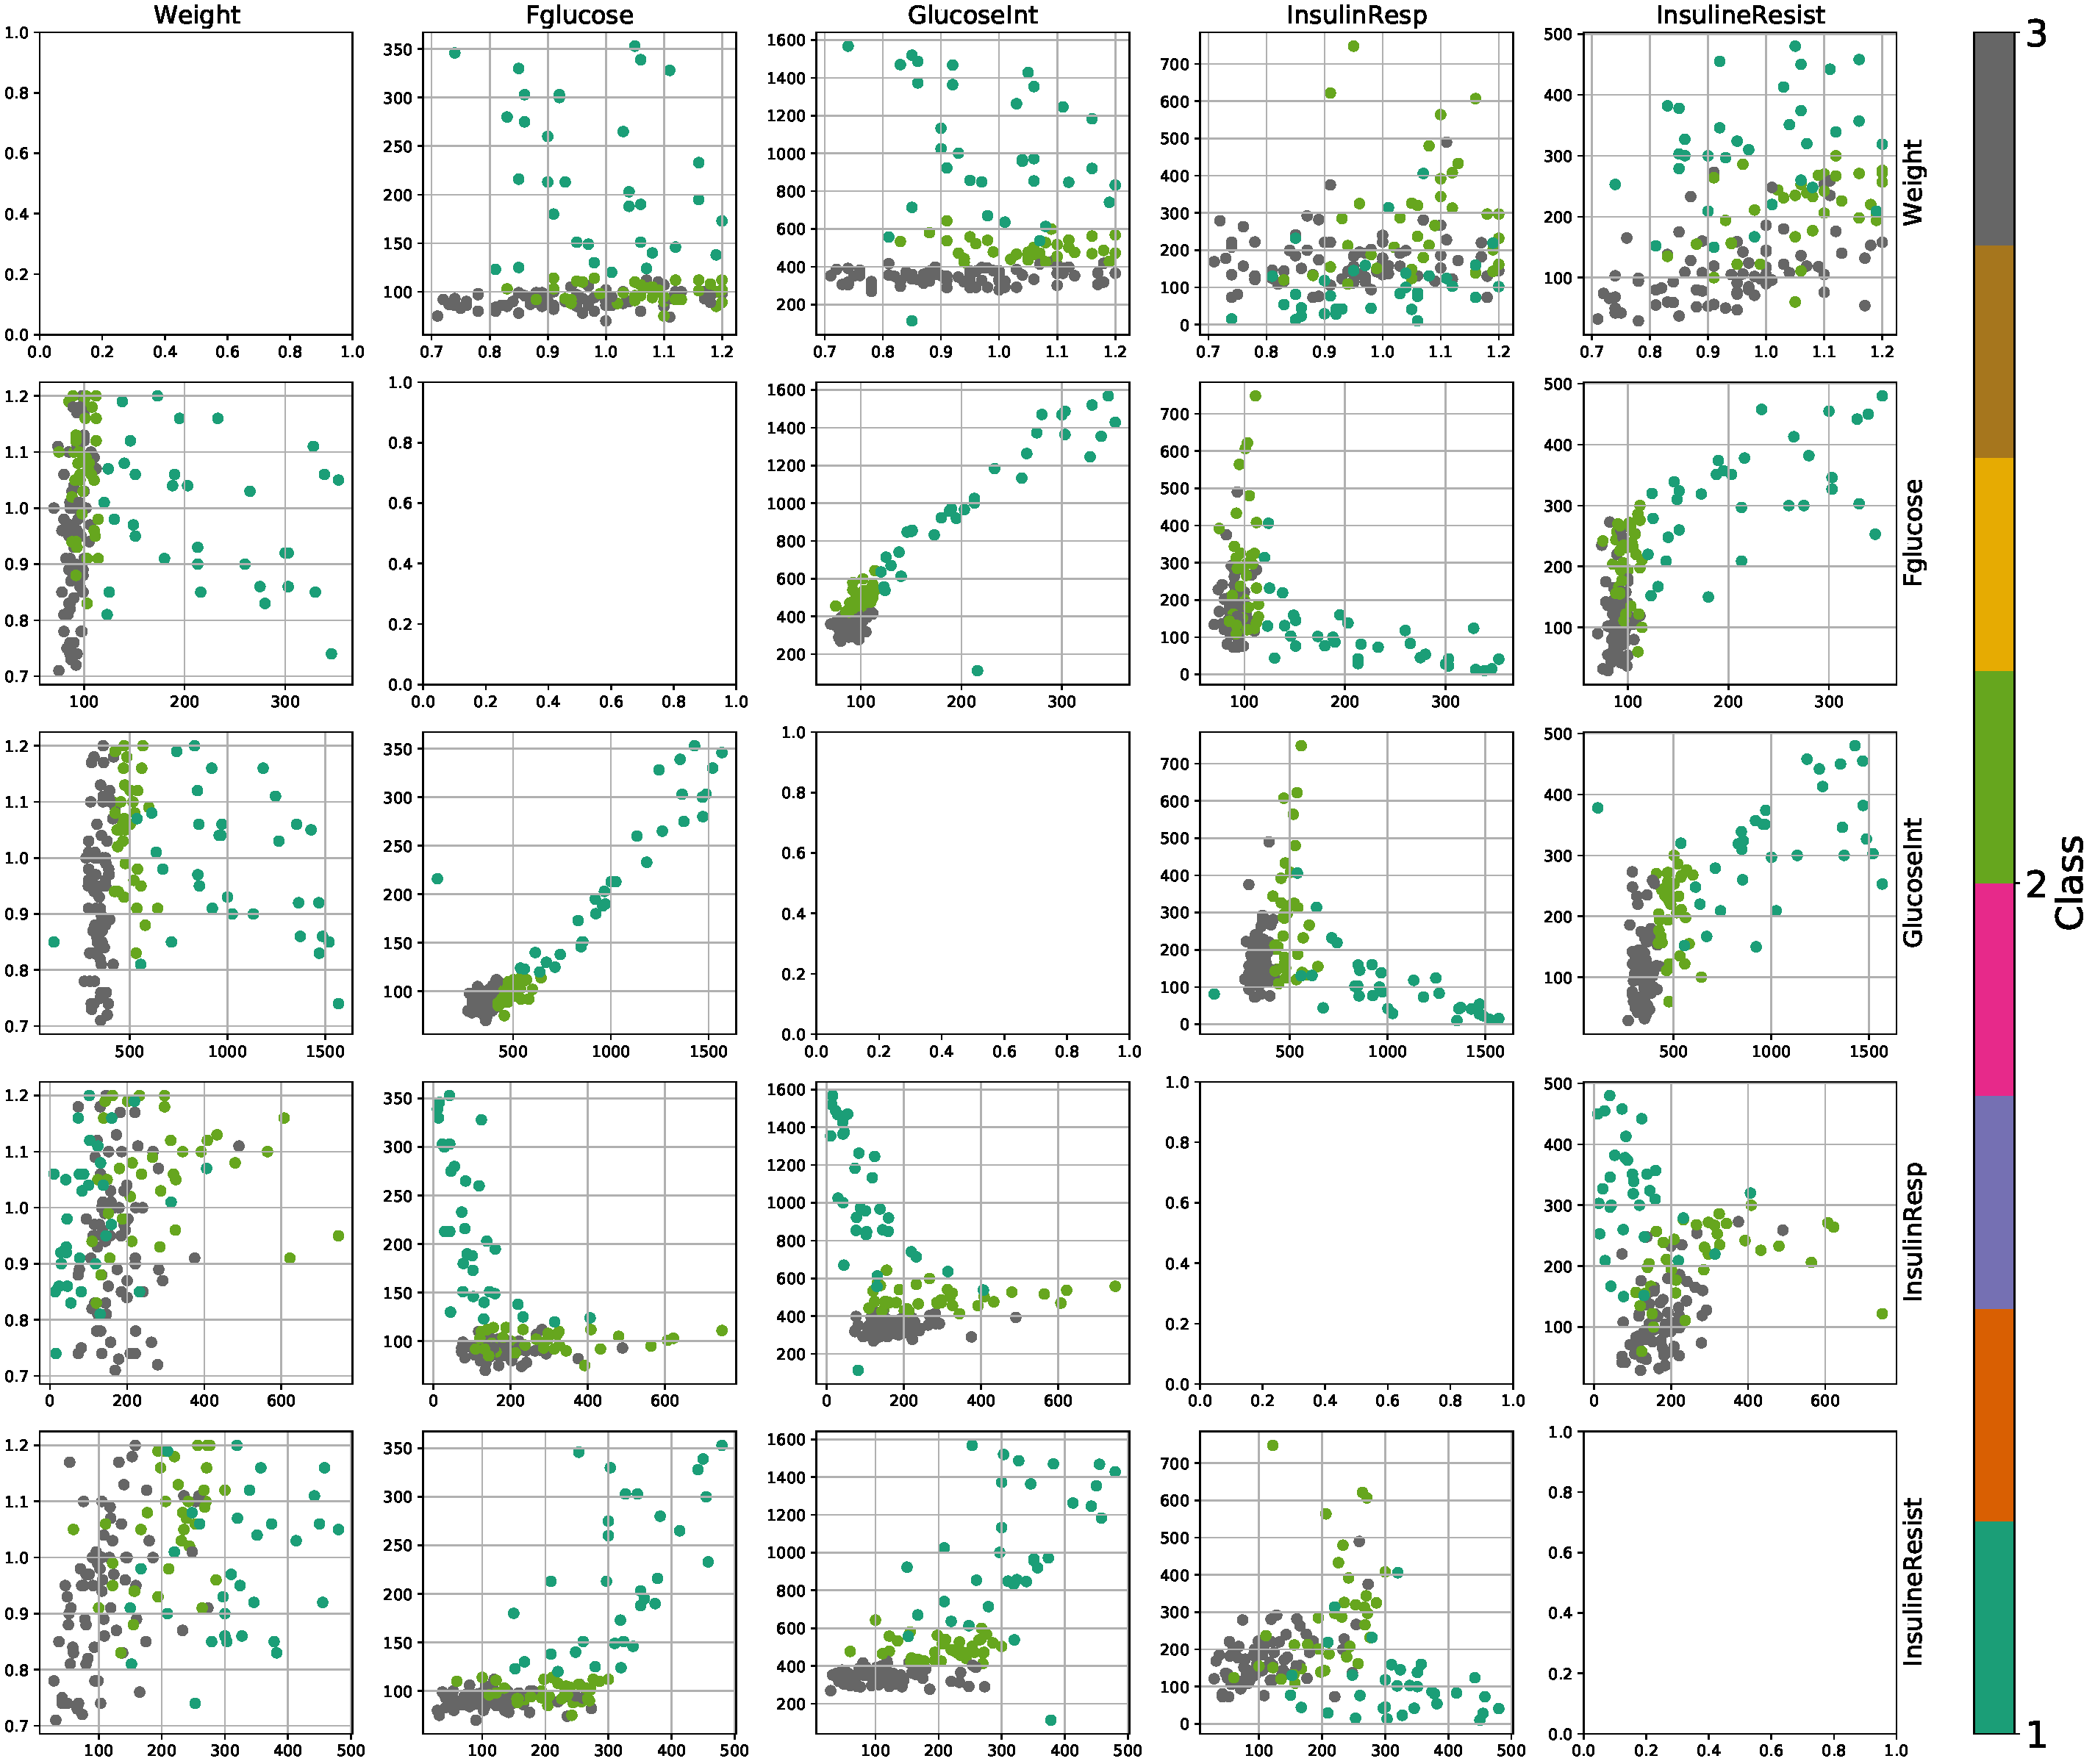
\includegraphics[width = 1.0\textwidth]{3-classes.pdf}
    \caption{Gráficas de una variable contra otra divididas en clases para las variables numéricas del problema 3}
    \label{3-classes}
\end{figure}
\begin{figure}[H]
    \centering
    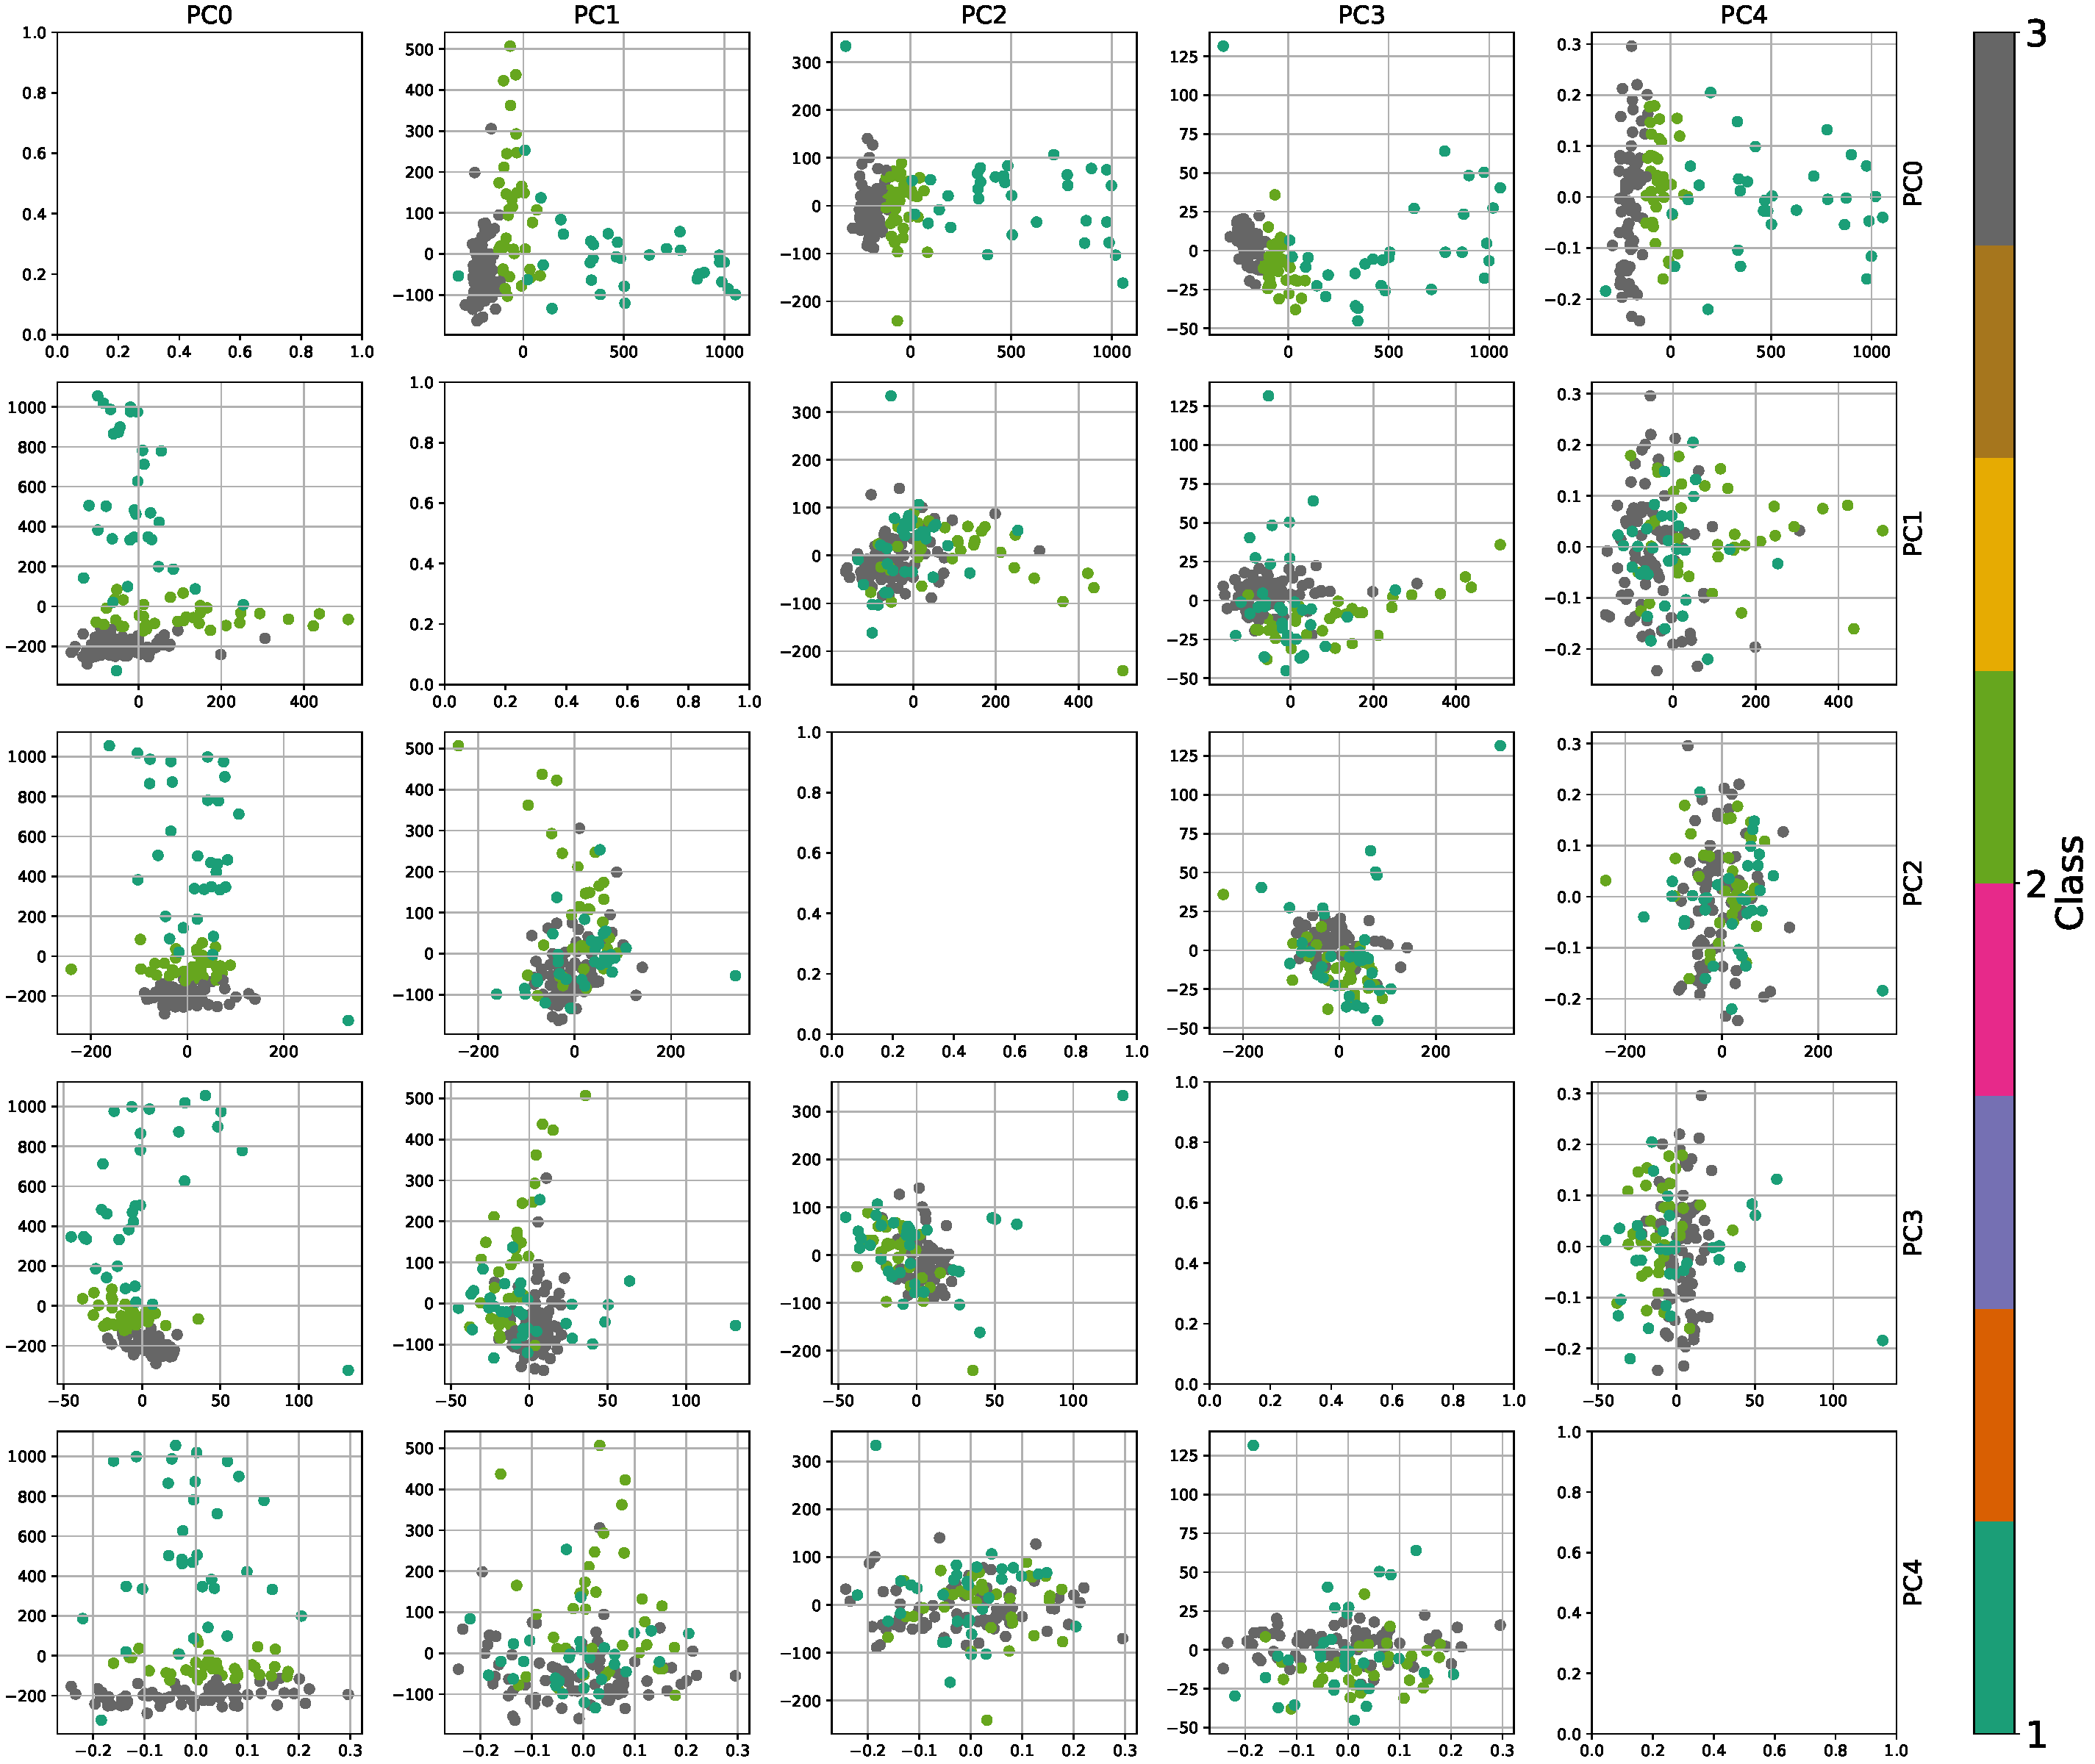
\includegraphics[width = 1.0\textwidth]{3-pca.pdf}
    \caption{Gráficas de una variable contra otra divididas en clases para las variables numéricas del problema 3}
    \label{3-pca}
\end{figure}
\begin{figure}[H]
    \centering
    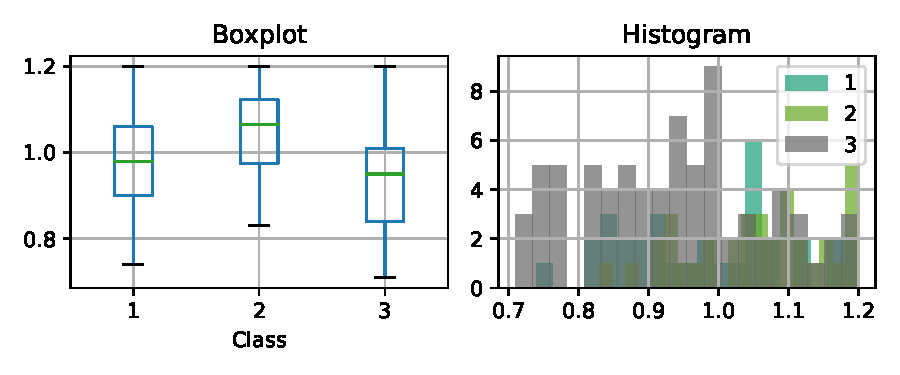
\includegraphics[width = 0.65\textwidth]{3-Weight-dist.pdf}
    \caption{Distribución de la variable ``Weight''}
    \label{3-Weight-dist}
\end{figure}
\begin{figure}[H]
    \centering
    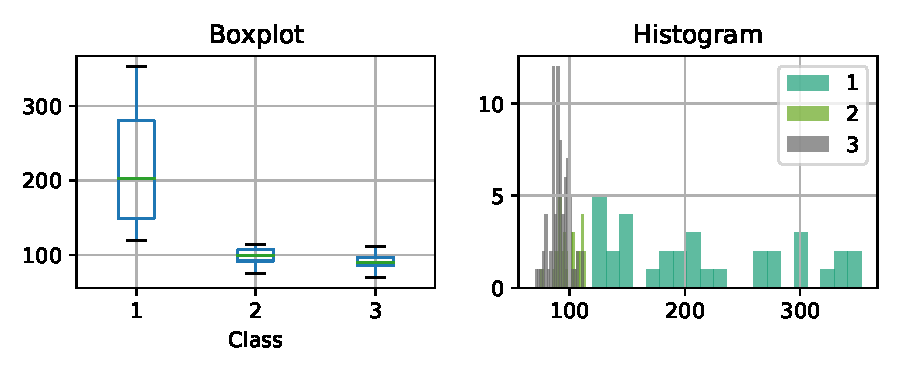
\includegraphics[width = 0.65\textwidth]{3-Fglucose-dist.pdf}
    \caption{Distribución de la variable ``Fglucose''}
    \label{3-Fglucose-dist}
\end{figure}
\begin{figure}[H]
    \centering
    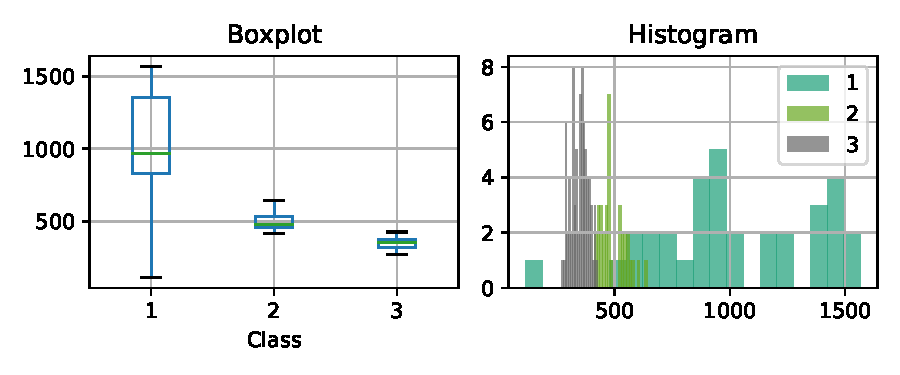
\includegraphics[width = 0.65\textwidth]{3-GlucoseInt-dist.pdf}
    \caption{Distribución de la variable ``Glucoseint''}
    \label{3-Glucoseint-dist}
\end{figure}
\begin{figure}[H]
    \centering
    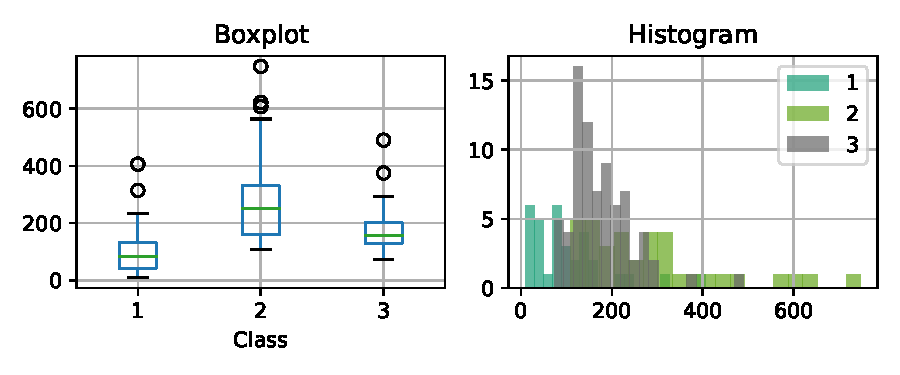
\includegraphics[width = 0.65\textwidth]{3-InsulinResp-dist.pdf}
    \caption{Distribución de la variable ``InsulinResp''}
    \label{3-InsulinResp-dist}
\end{figure}
\begin{figure}[H]
    \centering
    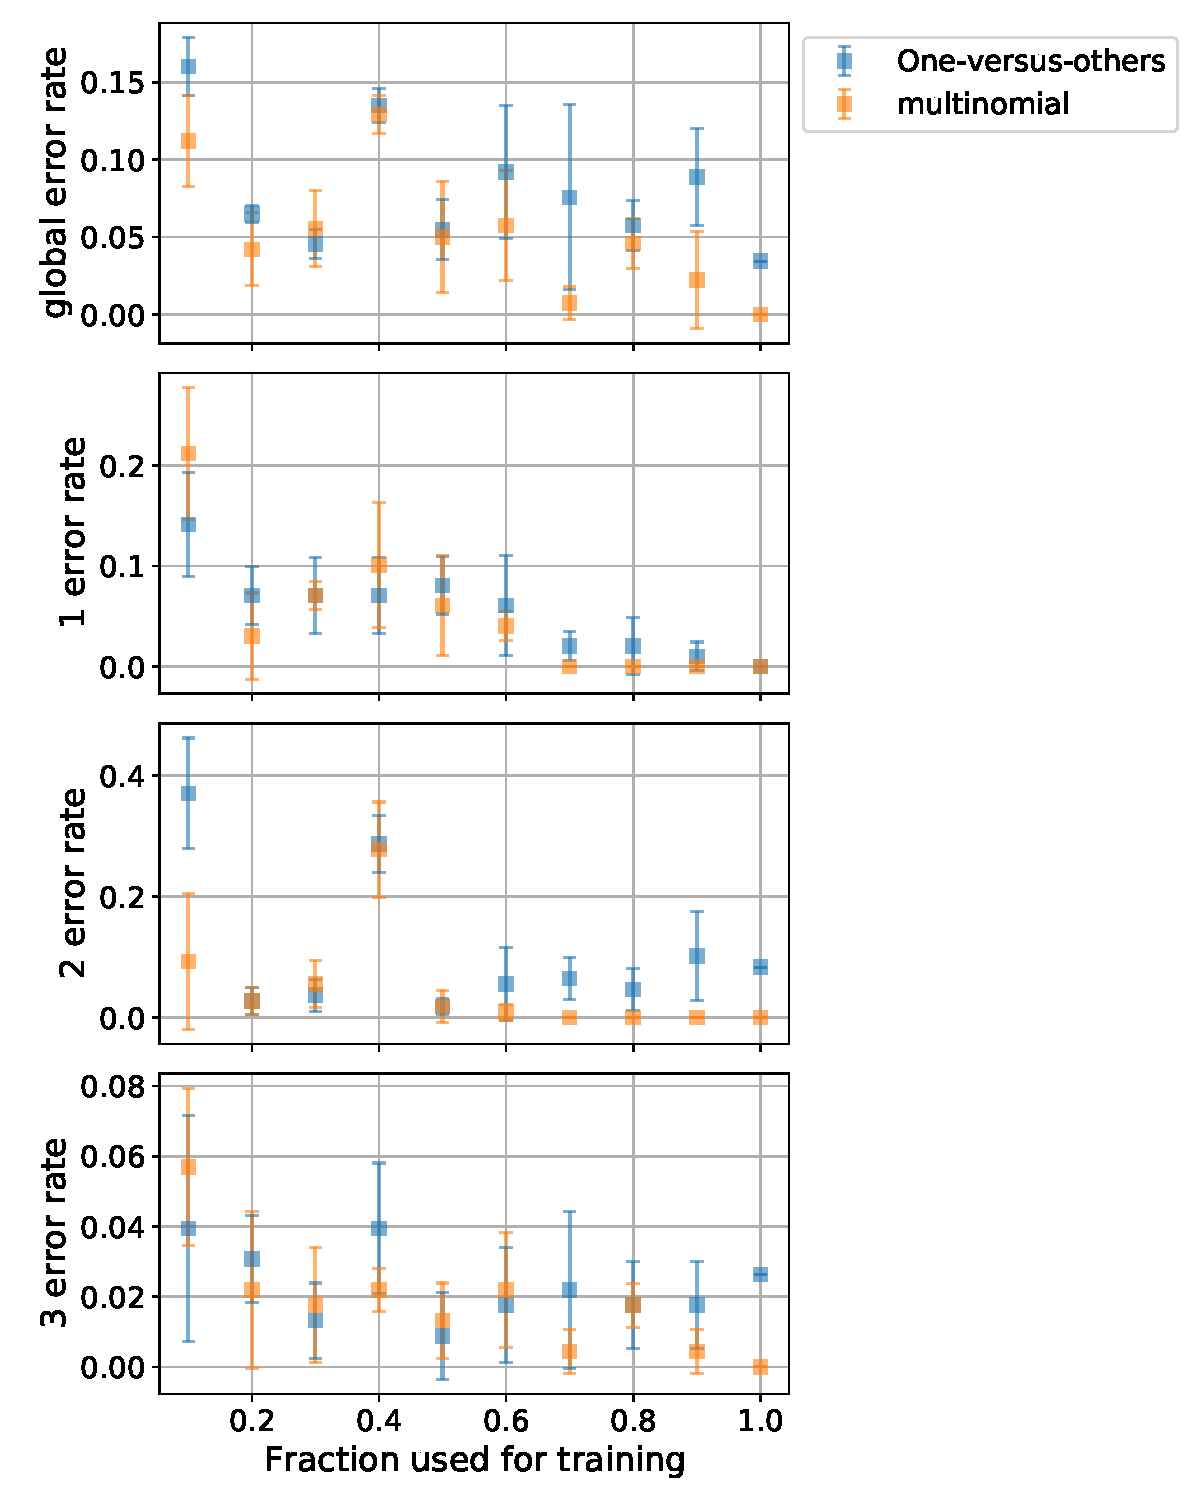
\includegraphics[width = 0.65\textwidth]{3-eq-sizeDependence.pdf}
    \caption{Distribución de la variable ``InsulineResist''}
    \label{3-eq-sizeDependence}
\end{figure}
\pagebreak
\section*{Anexo 3: Código en Python de los problemas}
\lstinputlisting[language=Python]{tarea3.py}
\printbibliography
\end{document}